
% Default to the notebook output style

    


% Inherit from the specified cell style.




    
\documentclass[11pt]{article}

    
    
    \usepackage[T1]{fontenc}
    % Nicer default font (+ math font) than Computer Modern for most use cases
    \usepackage{mathpazo}

    % Basic figure setup, for now with no caption control since it's done
    % automatically by Pandoc (which extracts ![](path) syntax from Markdown).
    \usepackage{graphicx}
    % We will generate all images so they have a width \maxwidth. This means
    % that they will get their normal width if they fit onto the page, but
    % are scaled down if they would overflow the margins.
    \makeatletter
    \def\maxwidth{\ifdim\Gin@nat@width>\linewidth\linewidth
    \else\Gin@nat@width\fi}
    \makeatother
    \let\Oldincludegraphics\includegraphics
    % Set max figure width to be 80% of text width, for now hardcoded.
    \renewcommand{\includegraphics}[1]{\Oldincludegraphics[width=.8\maxwidth]{#1}}
    % Ensure that by default, figures have no caption (until we provide a
    % proper Figure object with a Caption API and a way to capture that
    % in the conversion process - todo).
    \usepackage{caption}
    \DeclareCaptionLabelFormat{nolabel}{}
    \captionsetup{labelformat=nolabel}

    \usepackage{adjustbox} % Used to constrain images to a maximum size 
    \usepackage{xcolor} % Allow colors to be defined
    \usepackage{enumerate} % Needed for markdown enumerations to work
    \usepackage{geometry} % Used to adjust the document margins
    \usepackage{amsmath} % Equations
    \usepackage{amssymb} % Equations
    \usepackage{textcomp} % defines textquotesingle
    % Hack from http://tex.stackexchange.com/a/47451/13684:
    \AtBeginDocument{%
        \def\PYZsq{\textquotesingle}% Upright quotes in Pygmentized code
    }
    \usepackage{upquote} % Upright quotes for verbatim code
    \usepackage{eurosym} % defines \euro
    \usepackage[mathletters]{ucs} % Extended unicode (utf-8) support
    \usepackage[utf8x]{inputenc} % Allow utf-8 characters in the tex document
    \usepackage{fancyvrb} % verbatim replacement that allows latex
    \usepackage{grffile} % extends the file name processing of package graphics 
                         % to support a larger range 
    % The hyperref package gives us a pdf with properly built
    % internal navigation ('pdf bookmarks' for the table of contents,
    % internal cross-reference links, web links for URLs, etc.)
    \usepackage{hyperref}
    \usepackage{longtable} % longtable support required by pandoc >1.10
    \usepackage{booktabs}  % table support for pandoc > 1.12.2
    \usepackage[inline]{enumitem} % IRkernel/repr support (it uses the enumerate* environment)
    \usepackage[normalem]{ulem} % ulem is needed to support strikethroughs (\sout)
                                % normalem makes italics be italics, not underlines
    

    
    
    % Colors for the hyperref package
    \definecolor{urlcolor}{rgb}{0,.145,.698}
    \definecolor{linkcolor}{rgb}{.71,0.21,0.01}
    \definecolor{citecolor}{rgb}{.12,.54,.11}

    % ANSI colors
    \definecolor{ansi-black}{HTML}{3E424D}
    \definecolor{ansi-black-intense}{HTML}{282C36}
    \definecolor{ansi-red}{HTML}{E75C58}
    \definecolor{ansi-red-intense}{HTML}{B22B31}
    \definecolor{ansi-green}{HTML}{00A250}
    \definecolor{ansi-green-intense}{HTML}{007427}
    \definecolor{ansi-yellow}{HTML}{DDB62B}
    \definecolor{ansi-yellow-intense}{HTML}{B27D12}
    \definecolor{ansi-blue}{HTML}{208FFB}
    \definecolor{ansi-blue-intense}{HTML}{0065CA}
    \definecolor{ansi-magenta}{HTML}{D160C4}
    \definecolor{ansi-magenta-intense}{HTML}{A03196}
    \definecolor{ansi-cyan}{HTML}{60C6C8}
    \definecolor{ansi-cyan-intense}{HTML}{258F8F}
    \definecolor{ansi-white}{HTML}{C5C1B4}
    \definecolor{ansi-white-intense}{HTML}{A1A6B2}

    % commands and environments needed by pandoc snippets
    % extracted from the output of `pandoc -s`
    \providecommand{\tightlist}{%
      \setlength{\itemsep}{0pt}\setlength{\parskip}{0pt}}
    \DefineVerbatimEnvironment{Highlighting}{Verbatim}{commandchars=\\\{\}}
    % Add ',fontsize=\small' for more characters per line
    \newenvironment{Shaded}{}{}
    \newcommand{\KeywordTok}[1]{\textcolor[rgb]{0.00,0.44,0.13}{\textbf{{#1}}}}
    \newcommand{\DataTypeTok}[1]{\textcolor[rgb]{0.56,0.13,0.00}{{#1}}}
    \newcommand{\DecValTok}[1]{\textcolor[rgb]{0.25,0.63,0.44}{{#1}}}
    \newcommand{\BaseNTok}[1]{\textcolor[rgb]{0.25,0.63,0.44}{{#1}}}
    \newcommand{\FloatTok}[1]{\textcolor[rgb]{0.25,0.63,0.44}{{#1}}}
    \newcommand{\CharTok}[1]{\textcolor[rgb]{0.25,0.44,0.63}{{#1}}}
    \newcommand{\StringTok}[1]{\textcolor[rgb]{0.25,0.44,0.63}{{#1}}}
    \newcommand{\CommentTok}[1]{\textcolor[rgb]{0.38,0.63,0.69}{\textit{{#1}}}}
    \newcommand{\OtherTok}[1]{\textcolor[rgb]{0.00,0.44,0.13}{{#1}}}
    \newcommand{\AlertTok}[1]{\textcolor[rgb]{1.00,0.00,0.00}{\textbf{{#1}}}}
    \newcommand{\FunctionTok}[1]{\textcolor[rgb]{0.02,0.16,0.49}{{#1}}}
    \newcommand{\RegionMarkerTok}[1]{{#1}}
    \newcommand{\ErrorTok}[1]{\textcolor[rgb]{1.00,0.00,0.00}{\textbf{{#1}}}}
    \newcommand{\NormalTok}[1]{{#1}}
    
    % Additional commands for more recent versions of Pandoc
    \newcommand{\ConstantTok}[1]{\textcolor[rgb]{0.53,0.00,0.00}{{#1}}}
    \newcommand{\SpecialCharTok}[1]{\textcolor[rgb]{0.25,0.44,0.63}{{#1}}}
    \newcommand{\VerbatimStringTok}[1]{\textcolor[rgb]{0.25,0.44,0.63}{{#1}}}
    \newcommand{\SpecialStringTok}[1]{\textcolor[rgb]{0.73,0.40,0.53}{{#1}}}
    \newcommand{\ImportTok}[1]{{#1}}
    \newcommand{\DocumentationTok}[1]{\textcolor[rgb]{0.73,0.13,0.13}{\textit{{#1}}}}
    \newcommand{\AnnotationTok}[1]{\textcolor[rgb]{0.38,0.63,0.69}{\textbf{\textit{{#1}}}}}
    \newcommand{\CommentVarTok}[1]{\textcolor[rgb]{0.38,0.63,0.69}{\textbf{\textit{{#1}}}}}
    \newcommand{\VariableTok}[1]{\textcolor[rgb]{0.10,0.09,0.49}{{#1}}}
    \newcommand{\ControlFlowTok}[1]{\textcolor[rgb]{0.00,0.44,0.13}{\textbf{{#1}}}}
    \newcommand{\OperatorTok}[1]{\textcolor[rgb]{0.40,0.40,0.40}{{#1}}}
    \newcommand{\BuiltInTok}[1]{{#1}}
    \newcommand{\ExtensionTok}[1]{{#1}}
    \newcommand{\PreprocessorTok}[1]{\textcolor[rgb]{0.74,0.48,0.00}{{#1}}}
    \newcommand{\AttributeTok}[1]{\textcolor[rgb]{0.49,0.56,0.16}{{#1}}}
    \newcommand{\InformationTok}[1]{\textcolor[rgb]{0.38,0.63,0.69}{\textbf{\textit{{#1}}}}}
    \newcommand{\WarningTok}[1]{\textcolor[rgb]{0.38,0.63,0.69}{\textbf{\textit{{#1}}}}}
    
    
    % Define a nice break command that doesn't care if a line doesn't already
    % exist.
    \def\br{\hspace*{\fill} \\* }
    % Math Jax compatability definitions
    \def\gt{>}
    \def\lt{<}
    % Document parameters
    \title{Untitled}
    
    
    

    % Pygments definitions
    
\makeatletter
\def\PY@reset{\let\PY@it=\relax \let\PY@bf=\relax%
    \let\PY@ul=\relax \let\PY@tc=\relax%
    \let\PY@bc=\relax \let\PY@ff=\relax}
\def\PY@tok#1{\csname PY@tok@#1\endcsname}
\def\PY@toks#1+{\ifx\relax#1\empty\else%
    \PY@tok{#1}\expandafter\PY@toks\fi}
\def\PY@do#1{\PY@bc{\PY@tc{\PY@ul{%
    \PY@it{\PY@bf{\PY@ff{#1}}}}}}}
\def\PY#1#2{\PY@reset\PY@toks#1+\relax+\PY@do{#2}}

\expandafter\def\csname PY@tok@w\endcsname{\def\PY@tc##1{\textcolor[rgb]{0.73,0.73,0.73}{##1}}}
\expandafter\def\csname PY@tok@c\endcsname{\let\PY@it=\textit\def\PY@tc##1{\textcolor[rgb]{0.25,0.50,0.50}{##1}}}
\expandafter\def\csname PY@tok@cp\endcsname{\def\PY@tc##1{\textcolor[rgb]{0.74,0.48,0.00}{##1}}}
\expandafter\def\csname PY@tok@k\endcsname{\let\PY@bf=\textbf\def\PY@tc##1{\textcolor[rgb]{0.00,0.50,0.00}{##1}}}
\expandafter\def\csname PY@tok@kp\endcsname{\def\PY@tc##1{\textcolor[rgb]{0.00,0.50,0.00}{##1}}}
\expandafter\def\csname PY@tok@kt\endcsname{\def\PY@tc##1{\textcolor[rgb]{0.69,0.00,0.25}{##1}}}
\expandafter\def\csname PY@tok@o\endcsname{\def\PY@tc##1{\textcolor[rgb]{0.40,0.40,0.40}{##1}}}
\expandafter\def\csname PY@tok@ow\endcsname{\let\PY@bf=\textbf\def\PY@tc##1{\textcolor[rgb]{0.67,0.13,1.00}{##1}}}
\expandafter\def\csname PY@tok@nb\endcsname{\def\PY@tc##1{\textcolor[rgb]{0.00,0.50,0.00}{##1}}}
\expandafter\def\csname PY@tok@nf\endcsname{\def\PY@tc##1{\textcolor[rgb]{0.00,0.00,1.00}{##1}}}
\expandafter\def\csname PY@tok@nc\endcsname{\let\PY@bf=\textbf\def\PY@tc##1{\textcolor[rgb]{0.00,0.00,1.00}{##1}}}
\expandafter\def\csname PY@tok@nn\endcsname{\let\PY@bf=\textbf\def\PY@tc##1{\textcolor[rgb]{0.00,0.00,1.00}{##1}}}
\expandafter\def\csname PY@tok@ne\endcsname{\let\PY@bf=\textbf\def\PY@tc##1{\textcolor[rgb]{0.82,0.25,0.23}{##1}}}
\expandafter\def\csname PY@tok@nv\endcsname{\def\PY@tc##1{\textcolor[rgb]{0.10,0.09,0.49}{##1}}}
\expandafter\def\csname PY@tok@no\endcsname{\def\PY@tc##1{\textcolor[rgb]{0.53,0.00,0.00}{##1}}}
\expandafter\def\csname PY@tok@nl\endcsname{\def\PY@tc##1{\textcolor[rgb]{0.63,0.63,0.00}{##1}}}
\expandafter\def\csname PY@tok@ni\endcsname{\let\PY@bf=\textbf\def\PY@tc##1{\textcolor[rgb]{0.60,0.60,0.60}{##1}}}
\expandafter\def\csname PY@tok@na\endcsname{\def\PY@tc##1{\textcolor[rgb]{0.49,0.56,0.16}{##1}}}
\expandafter\def\csname PY@tok@nt\endcsname{\let\PY@bf=\textbf\def\PY@tc##1{\textcolor[rgb]{0.00,0.50,0.00}{##1}}}
\expandafter\def\csname PY@tok@nd\endcsname{\def\PY@tc##1{\textcolor[rgb]{0.67,0.13,1.00}{##1}}}
\expandafter\def\csname PY@tok@s\endcsname{\def\PY@tc##1{\textcolor[rgb]{0.73,0.13,0.13}{##1}}}
\expandafter\def\csname PY@tok@sd\endcsname{\let\PY@it=\textit\def\PY@tc##1{\textcolor[rgb]{0.73,0.13,0.13}{##1}}}
\expandafter\def\csname PY@tok@si\endcsname{\let\PY@bf=\textbf\def\PY@tc##1{\textcolor[rgb]{0.73,0.40,0.53}{##1}}}
\expandafter\def\csname PY@tok@se\endcsname{\let\PY@bf=\textbf\def\PY@tc##1{\textcolor[rgb]{0.73,0.40,0.13}{##1}}}
\expandafter\def\csname PY@tok@sr\endcsname{\def\PY@tc##1{\textcolor[rgb]{0.73,0.40,0.53}{##1}}}
\expandafter\def\csname PY@tok@ss\endcsname{\def\PY@tc##1{\textcolor[rgb]{0.10,0.09,0.49}{##1}}}
\expandafter\def\csname PY@tok@sx\endcsname{\def\PY@tc##1{\textcolor[rgb]{0.00,0.50,0.00}{##1}}}
\expandafter\def\csname PY@tok@m\endcsname{\def\PY@tc##1{\textcolor[rgb]{0.40,0.40,0.40}{##1}}}
\expandafter\def\csname PY@tok@gh\endcsname{\let\PY@bf=\textbf\def\PY@tc##1{\textcolor[rgb]{0.00,0.00,0.50}{##1}}}
\expandafter\def\csname PY@tok@gu\endcsname{\let\PY@bf=\textbf\def\PY@tc##1{\textcolor[rgb]{0.50,0.00,0.50}{##1}}}
\expandafter\def\csname PY@tok@gd\endcsname{\def\PY@tc##1{\textcolor[rgb]{0.63,0.00,0.00}{##1}}}
\expandafter\def\csname PY@tok@gi\endcsname{\def\PY@tc##1{\textcolor[rgb]{0.00,0.63,0.00}{##1}}}
\expandafter\def\csname PY@tok@gr\endcsname{\def\PY@tc##1{\textcolor[rgb]{1.00,0.00,0.00}{##1}}}
\expandafter\def\csname PY@tok@ge\endcsname{\let\PY@it=\textit}
\expandafter\def\csname PY@tok@gs\endcsname{\let\PY@bf=\textbf}
\expandafter\def\csname PY@tok@gp\endcsname{\let\PY@bf=\textbf\def\PY@tc##1{\textcolor[rgb]{0.00,0.00,0.50}{##1}}}
\expandafter\def\csname PY@tok@go\endcsname{\def\PY@tc##1{\textcolor[rgb]{0.53,0.53,0.53}{##1}}}
\expandafter\def\csname PY@tok@gt\endcsname{\def\PY@tc##1{\textcolor[rgb]{0.00,0.27,0.87}{##1}}}
\expandafter\def\csname PY@tok@err\endcsname{\def\PY@bc##1{\setlength{\fboxsep}{0pt}\fcolorbox[rgb]{1.00,0.00,0.00}{1,1,1}{\strut ##1}}}
\expandafter\def\csname PY@tok@kc\endcsname{\let\PY@bf=\textbf\def\PY@tc##1{\textcolor[rgb]{0.00,0.50,0.00}{##1}}}
\expandafter\def\csname PY@tok@kd\endcsname{\let\PY@bf=\textbf\def\PY@tc##1{\textcolor[rgb]{0.00,0.50,0.00}{##1}}}
\expandafter\def\csname PY@tok@kn\endcsname{\let\PY@bf=\textbf\def\PY@tc##1{\textcolor[rgb]{0.00,0.50,0.00}{##1}}}
\expandafter\def\csname PY@tok@kr\endcsname{\let\PY@bf=\textbf\def\PY@tc##1{\textcolor[rgb]{0.00,0.50,0.00}{##1}}}
\expandafter\def\csname PY@tok@bp\endcsname{\def\PY@tc##1{\textcolor[rgb]{0.00,0.50,0.00}{##1}}}
\expandafter\def\csname PY@tok@fm\endcsname{\def\PY@tc##1{\textcolor[rgb]{0.00,0.00,1.00}{##1}}}
\expandafter\def\csname PY@tok@vc\endcsname{\def\PY@tc##1{\textcolor[rgb]{0.10,0.09,0.49}{##1}}}
\expandafter\def\csname PY@tok@vg\endcsname{\def\PY@tc##1{\textcolor[rgb]{0.10,0.09,0.49}{##1}}}
\expandafter\def\csname PY@tok@vi\endcsname{\def\PY@tc##1{\textcolor[rgb]{0.10,0.09,0.49}{##1}}}
\expandafter\def\csname PY@tok@vm\endcsname{\def\PY@tc##1{\textcolor[rgb]{0.10,0.09,0.49}{##1}}}
\expandafter\def\csname PY@tok@sa\endcsname{\def\PY@tc##1{\textcolor[rgb]{0.73,0.13,0.13}{##1}}}
\expandafter\def\csname PY@tok@sb\endcsname{\def\PY@tc##1{\textcolor[rgb]{0.73,0.13,0.13}{##1}}}
\expandafter\def\csname PY@tok@sc\endcsname{\def\PY@tc##1{\textcolor[rgb]{0.73,0.13,0.13}{##1}}}
\expandafter\def\csname PY@tok@dl\endcsname{\def\PY@tc##1{\textcolor[rgb]{0.73,0.13,0.13}{##1}}}
\expandafter\def\csname PY@tok@s2\endcsname{\def\PY@tc##1{\textcolor[rgb]{0.73,0.13,0.13}{##1}}}
\expandafter\def\csname PY@tok@sh\endcsname{\def\PY@tc##1{\textcolor[rgb]{0.73,0.13,0.13}{##1}}}
\expandafter\def\csname PY@tok@s1\endcsname{\def\PY@tc##1{\textcolor[rgb]{0.73,0.13,0.13}{##1}}}
\expandafter\def\csname PY@tok@mb\endcsname{\def\PY@tc##1{\textcolor[rgb]{0.40,0.40,0.40}{##1}}}
\expandafter\def\csname PY@tok@mf\endcsname{\def\PY@tc##1{\textcolor[rgb]{0.40,0.40,0.40}{##1}}}
\expandafter\def\csname PY@tok@mh\endcsname{\def\PY@tc##1{\textcolor[rgb]{0.40,0.40,0.40}{##1}}}
\expandafter\def\csname PY@tok@mi\endcsname{\def\PY@tc##1{\textcolor[rgb]{0.40,0.40,0.40}{##1}}}
\expandafter\def\csname PY@tok@il\endcsname{\def\PY@tc##1{\textcolor[rgb]{0.40,0.40,0.40}{##1}}}
\expandafter\def\csname PY@tok@mo\endcsname{\def\PY@tc##1{\textcolor[rgb]{0.40,0.40,0.40}{##1}}}
\expandafter\def\csname PY@tok@ch\endcsname{\let\PY@it=\textit\def\PY@tc##1{\textcolor[rgb]{0.25,0.50,0.50}{##1}}}
\expandafter\def\csname PY@tok@cm\endcsname{\let\PY@it=\textit\def\PY@tc##1{\textcolor[rgb]{0.25,0.50,0.50}{##1}}}
\expandafter\def\csname PY@tok@cpf\endcsname{\let\PY@it=\textit\def\PY@tc##1{\textcolor[rgb]{0.25,0.50,0.50}{##1}}}
\expandafter\def\csname PY@tok@c1\endcsname{\let\PY@it=\textit\def\PY@tc##1{\textcolor[rgb]{0.25,0.50,0.50}{##1}}}
\expandafter\def\csname PY@tok@cs\endcsname{\let\PY@it=\textit\def\PY@tc##1{\textcolor[rgb]{0.25,0.50,0.50}{##1}}}

\def\PYZbs{\char`\\}
\def\PYZus{\char`\_}
\def\PYZob{\char`\{}
\def\PYZcb{\char`\}}
\def\PYZca{\char`\^}
\def\PYZam{\char`\&}
\def\PYZlt{\char`\<}
\def\PYZgt{\char`\>}
\def\PYZsh{\char`\#}
\def\PYZpc{\char`\%}
\def\PYZdl{\char`\$}
\def\PYZhy{\char`\-}
\def\PYZsq{\char`\'}
\def\PYZdq{\char`\"}
\def\PYZti{\char`\~}
% for compatibility with earlier versions
\def\PYZat{@}
\def\PYZlb{[}
\def\PYZrb{]}
\makeatother


    % Exact colors from NB
    \definecolor{incolor}{rgb}{0.0, 0.0, 0.5}
    \definecolor{outcolor}{rgb}{0.545, 0.0, 0.0}



    
    % Prevent overflowing lines due to hard-to-break entities
    \sloppy 
    % Setup hyperref package
    \hypersetup{
      breaklinks=true,  % so long urls are correctly broken across lines
      colorlinks=true,
      urlcolor=urlcolor,
      linkcolor=linkcolor,
      citecolor=citecolor,
      }
    % Slightly bigger margins than the latex defaults
    
    \geometry{verbose,tmargin=1in,bmargin=1in,lmargin=1in,rmargin=1in}
    
    

    \begin{document}
    
    
    \maketitle
    
    

    
    \subsection{Multimodal Transfer: A Hierarchical Deep Convolutional
Neural Network for Fast Artistic Style
Transfer}\label{multimodal-transfer-a-hierarchical-deep-convolutional-neural-network-for-fast-artistic-style-transfer}

    Assignment 1: Marc Schmid Student No 13349752 1 paper 2 gats 3 johnson

    \section{Content}\label{content}

\subsection{Introduction}\label{introduction}

The paper is of the area of deep learning for computer vision. It
investigates new generative neural network models to transfer artistic
styles onto arbitrary images. There are already online learning
algorithms, but they do not represent the style transfer correctly as
they fail to display the style in local regions of the picture. The
paper is mainly based on the work of L. A. Gatys, A. S. Ecker, and M.
Bethge. 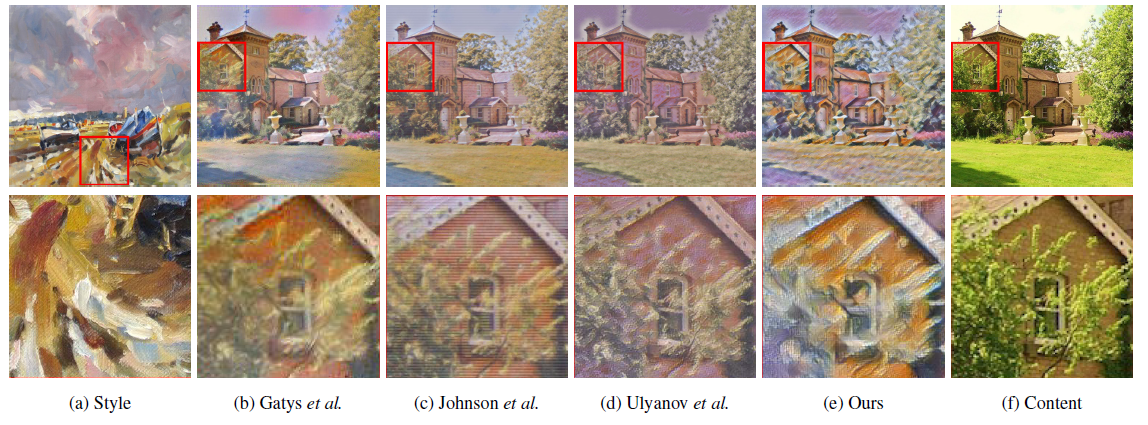
\includegraphics{firstPic.png} Top row: (a) The style guide is
"At the Close of Day" by Tomas King, and (f) is the content image. (b)
is the result of Gatys et al's optimization-based method. (Result size
is 512 due to memory limitation of the method) (c), (d) and (e) are
results generated by different feed-forward networks (all are of size
1024). Bottom row: the zoom-in display of the regions enclosed in the
red boxes from the top row. As can be seen, all results are repainted
with the color of the style image. However, a closer examination shows
that the brush strokes are not captured well in (c) and (d). The zoom-in
region in (b) is a little blurry. Comparing with the others, our
multimodal transfer (e) is capable of simulating more closely the
brushwork of the original artwork on high-resolution images.(From
{[}1{]})

Image style transfer using convolutional neural networks, where a
pre-trained deep learning network for visual recognition is used to
capture both style and content representations. They reduced the
computing time of the neural network by training it offline and
introducing a new hirarchical deep convolutional neural network
architecture. This helps to fasten the computation of style transfers in
software like Adobe Photoshop. Through the fully convolutional network
it is guaranteed to process pictures of different sizes (but it has to
have a minimal size, otherwise a 1 by 1 convolution will eventually
crash somewhere in the neural net). They introduce a new structure in
the first neural network they use, where they differentiate in color
scheme and ilumination, as visual perception is far more sensitive to
changes in ilumination than in color. They proof in experiments that
they achieve better results for the style transfer than in traditional
CNN-Architectures.

    \subsection{Network Architecture}\label{network-architecture}

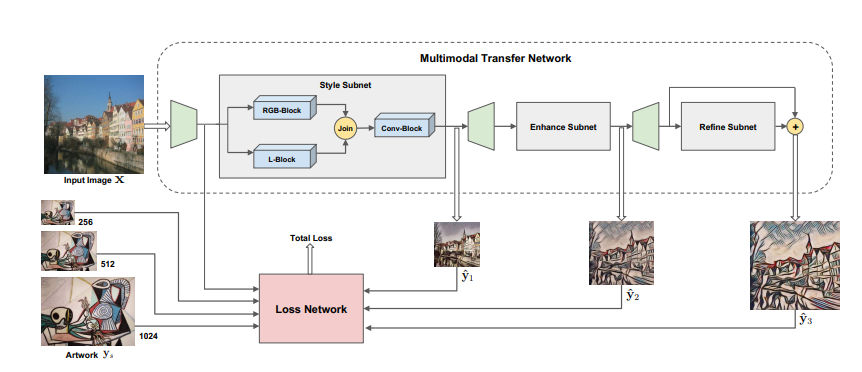
\includegraphics{overarch.png} The overall architecture of the neural
network is structured into 3 subnets (MT Network). The Style Subnet, the
Enhance Subnet and the Refine Subnet. This network architecture was
chosen because its difficult to optimally adjust textures to a variety
of styles. The network takes an image as input and generates an output
image for each subnet with increasing resolution. These output images
are then taken as inputs to the loss network to calculate a styleization
loss for each image. Afterwards the total loss is a weighted combination
of all stylization losses. The subnet prediction is defined as
\[X_k= f(\omega_k, x)\], where \(X_k\) is the prediction of the k-th
network, \(\omega_k\) are the parameters of the k-th network, \(x\) is
the input image and \(f()\) is the corresponding neural network
architecture.

\subsubsection{Style Subnet}\label{style-subnet}

As visual perception is far more sensitive to iluminance than color, the
Style Subnet adresses the three color channels (in the RGB-Block) as
well as the luminance channels (in the L-Block). The feature maps
computed by those both nets are than concatinated in the depth dimension
und further processed by the following Convolution Block. The goal of
the Style Subnet is to preserve the content and to adjust the textures
to the style a lot. The RGB and L Block consist of three convolutional
layers followed by three instance normalization layers and ReLU
activation functions respectively, followed by three residual blocks.
After the concatination of the two blocks there follows an upsampling
convolutional layer structure, to reach the right size of the image.

\subsubsection{Enhance Subnet and Refine
Subnet}\label{enhance-subnet-and-refine-subnet}

The job of the Enhance Subnet and Refine Subnet is to furher change the
style of the picture, but less then the Style Subnet. The Enhance Subnet
as well as the Refine Subnet are fully convolutional neural networks
which upsample the the images to the size of 512 and 1024 respectively.
The Enhance Subnet consists of 4 convolutional layers, 6 residual
blocks, followed by a upsampling convolutional structure. The Refine
Subnet is embodied similar with 4 convolutional layers, 3 residual
blocks as well an upsampling structure, so that the image matches the
target.

\paragraph{Comparison of the
Refinement}\label{comparison-of-the-refinement}

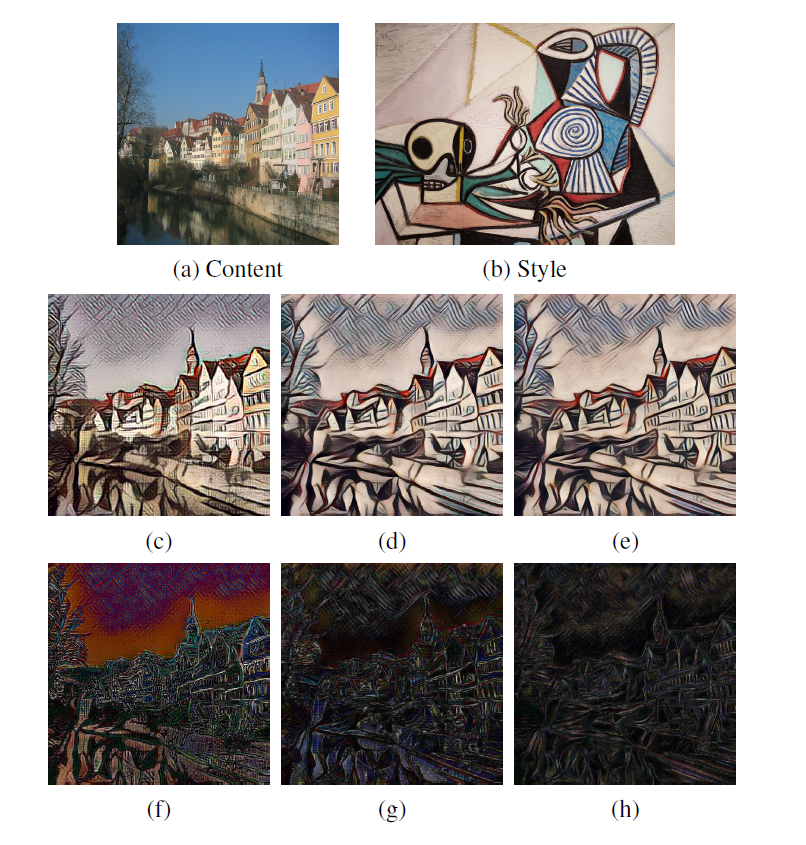
\includegraphics{refstruc.png} (a) is the content image and (b) is the
style image. (c)(d)(e) show the outputs of the three subnets,
\(\hat{y}_1\), \(\hat{y}_2\) and \(\hat{y}_3\), whose sizes are 256, 512
and 1024 respectively. The third row depicts the absolute difference
between: (f) the content image and the output image \(\hat{y}_1\), (g)
the output images \(\hat{y}_1\) and \(\hat{y}_2\), and (h) the output
images \(\hat{y}_2\) and \(\hat{y}_3\).(From {[}1{]})

We can see that the total difference between the pictures is decreasing
in each subnet. So that the Style Subnet changes the content picture a
lot, while the enhance and refine subnets focus on detail adaption.

\subsection{Mathematical Foundations and Learning
Schemes}\label{mathematical-foundations-and-learning-schemes}

As explained in the network architecture, the multimodal CNN takes an
imput image and returns 3 output images. These output images are the put
into the loss network which calculates stylization losses. The loss
network is the VGG16 (in the implementation I used the pretrained model
from torchvision).

\paragraph{Excursion: VGG16-NN Structure and use as Stylization Loss
Network}\label{excursion-vgg16-nn-structure-and-use-as-stylization-loss-network}

\begin{figure}
\centering
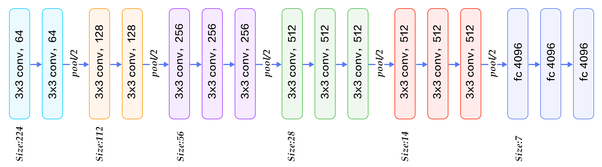
\includegraphics{vgg16_struct.png}
\caption{VGG16 Structure}
\end{figure}

The VGG16 Network was actually build for 224x224x3 pictures as a
classification task. It consists of twelve convolutional layers with max
pooling layers inbetween which extend to 512 channels in the last
convolution , before a few fully connected layers are used for
classification. In the MT Network the VGG16-Loss is expanded to a
Content Loss and Texture/Style Loss.

\subsubsection{Loss Function}\label{loss-function}

\begin{figure}
\centering
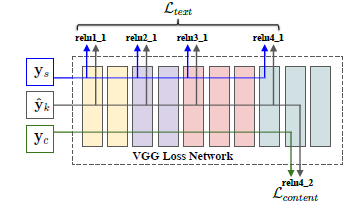
\includegraphics{loss_net.png}
\caption{VGG16 Loss Network}
\end{figure}

\paragraph{Content Loss}\label{content-loss}

Let \(\vec{p}\) and \(X\) be the original image and the generated image,
and \(P^l\) and \(F^l\) their respective feature representation in layer
l. The squared-error loss between the two feature representations is
defined as

\begin{equation}
 \mathcal{L}_{content}(\vec{p}, X, l ) = \frac{1}{2} \sum_{i,j}(F^l_{i,j}-P^l_{i,j})^2
\end{equation}

Thus, the content loss compares the feature difference for the
\textit(l)-th layer of the convolution of the VGG16. It is for sure a
good idea to compute the content loss in one of the last layers of the
VGG net, as in the first convolutional layers the standard features like
vertical and horizontal lines are covered. In the last convolution
layers more complex features get covered, so that the content really
gets compared, and not some superficial features.

\paragraph{Style Loss}\label{style-loss}

The Style loss consists of the correlations between the different filter
responses, where the expectation is taken over the spatial extent of the
feature maps. These feature correlations are given by the Gram matrix
\(G^l \in \mathcal{R}^{N_l\times N_l}\), where \(G^l_{ij}\) is the inner
product between the vectorised feature maps \(i\) and \(j\) in layer
\(l\): \[G^l_{i,j}= \sum_k F^l_{ik}F^l_{j,k}\] which equals:

\begin{equation}
G(x_1,\dots, x_n)=\begin{pmatrix} \langle x_1,x_1\rangle & \langle x_1,x_2\rangle &\dots & \langle x_1,x_n\rangle\\
 \langle x_2,x_1\rangle & \langle x_2,x_2\rangle &\dots & \langle x_2,x_n\rangle\\
\vdots&\vdots&\ddots&\vdots\\
 \langle x_n,x_1\rangle & \langle x_n,x_2\rangle &\dots & \langle x_n,x_n\rangle\end{pmatrix}.
\end{equation}

in matrix notation. By including the feature correlations of multiple
layers, a stationary, multi-scale representation of the input image is
obtained, which captures its texture information but not the global
arrangement. Therefore the texture function loss is defined as

\begin{equation}
 \mathcal{L}_{texture}(\vec{q}, X) = \sum_{l∈L}w_l(G^l(\vec{q})-G^l(X))^2
\end{equation}

with the amount of Layers chosen \(L\), generated picture \(X\) and
style target \(\vec{q}\), and a chosen weight for each layer \(w_l\).

Now it is up to the user to decide which weight of content and texture
loss is

\begin{equation}
\mathcal{L}_{style}(\vec{p},\vec{q}, X) =\alpha \mathcal{L}_{content}(\vec{p}, X, l ) +\beta \mathcal{L}_{texture}(\vec{q}, X)
\end{equation}

where \(\alpha\) and \(\beta\) are the weights of the content loss and
texture loss, respectively.

\paragraph{Hirarchical Stylization Loss
Function}\label{hirarchical-stylization-loss-function}

As the previously discussed part is nothing new, as it got already
presented at {[}2{]} the MT Network provides 3 outputs \(X_k\) with \$
k∈{[}1,2,3{]}\$ for the MT Network. Therefore multiple loss function get
computed which have to be combined. Thus, the hirarchical stylization
loss function \$\mathcal{L}\_H \$ is introduced. The loss function is a
sum of weighted loss function of the stylization losses:

\begin{equation}
\mathcal{L}_H = \sum_k \lambda_k \mathcal{L}_{style}(\vec{p}_k,\vec{q}_k, X_k) 
\end{equation}

where \(\lambda_k\) is the weight of the corresponding stylization loss.

To train the neural network, it is important to compute a gradient for
the backward pass. For each subnet (\(k\)) feature space \(\omega_k\) is
trained to minimize the parallel weighted stylization losses that are
computed from the outputs of the layer after the the layer of which the
actuall loss is taken. Thus, they defined the features as

\[\omega_k=argmin_{\omega_k}E_x\left[\sum_{i\geq k} \lambda_i \mathcal{L}^k_{style}(f(\omega_k,x),\vec p ,\vec q) \right]\]
The gradients get computed by

\[\delta \omega_k=\begin{cases}
(lambda_k \mathcal{L}^k_{style})'  \  & \text{if }k=K\\
(lambda_k \mathcal{L}^k_{style}, \delta \omega_{k+1})'  \  & \text{if} 1 \leq k \leq K\end{cases}\ \]

F. Meissen told me to add a regularization loss like in {[}3{]} for
better training results and to prevent overfitting, as I haven't trained
on the full Coco dataset, just on 50\% of the dataset.

\subsection{Used Layers}\label{used-layers}

(Just a short mention as they were not explained in the lecture)

\subsubsection{Convolutional Layer}\label{convolutional-layer}

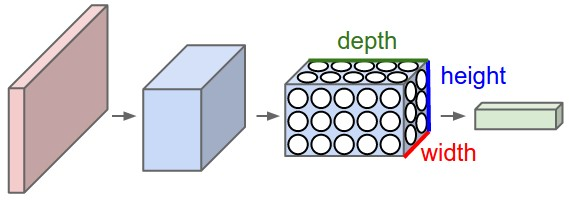
\includegraphics{cnn.jpeg} In this figure we can see a downsampling
structure of a convolution just by different filters and strides which
decreases the width and higth. The amount of filters increases the
depth.

In convolutional layers we use so called filters to connect the neurons.
The neurons are not all to all connected anymore, eather they are
dependend on their neighbors. In convolutions we use the fact that
pixels next to each other are somehow connected to each other. Through
weight sharing in convolutional layers

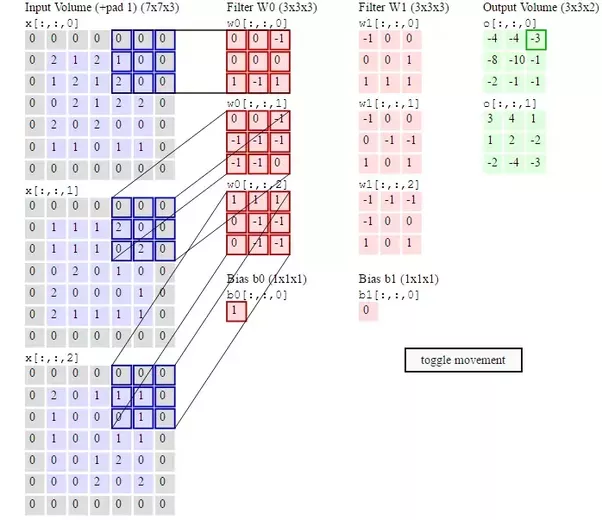
\includegraphics{conv_filter.png} In this figure we can see how two 3x3
filters/kernels work on a Input volumen of 7x7x3 with padding 1. You
swipe the kernels over the different depth levels. In general you start
at the upper left and take one step to the right until you reach the
other border. Then you slip one line down until you coverd the whole
picture.

\paragraph{Properties}\label{properties}

\subparagraph{Padding}\label{padding}

The padding p puts some numbers around of the border of the picture.
With it we can change the size of the output size.

\subparagraph{Spatial Extend}\label{spatial-extend}

The spatial extend F is the receptive field size of the convolution
layer neurons.

\subparagraph{Stride}\label{stride}

The stride s specifies how many pixels we move the filter in one step.
Stride 1 is common.

\subparagraph{Computation of the Output
Size}\label{computation-of-the-output-size}

The output size of the new convolutional volume can be computed, if the
stride, spatial extend, padding and the input width and hight are known:

\[W_2= \frac{W_1-F+2P}{S}+1\] \[H_2= \frac{H_1-F+2P}{S}+1\]

The Depth is just the amount of kernels used.

\subsubsection{Residual Block}\label{residual-block}

Deep neural networks suffer from vanishing or exploding gradient as well
as saturation of accuracy, dependant on the activaiton functions. Let us
consider a shallower architecture and its deeper counterpart that adds
more layers onto it. There exists a solution to the deeper model by
construction: the layers are copied from the learned shallower model,
and the added layers are identity mapping. The existence of this
constructed solution indicates that a deeper model should produce no
higher training error than its shallower counterpart.
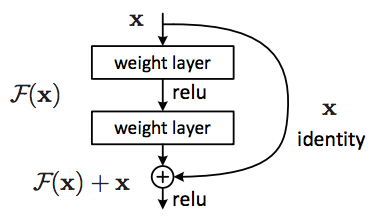
\includegraphics{res_struc.png}

Instead of hoping each stack of layers directly fits a desired
underlying mapping, we explicitly let these layers fit a residual
mapping. The original mapping is recast into \(F(x)+x\). We hypothesize
that it is easier to optimize the residual mapping than to optimize the
original, unreferenced mapping. To the extreme, if an identity mapping
were optimal, it would be easier to push the residual to zero than to
fit an identity mapping by a stack of nonlinear layers.

\subsubsection{Instance Normalization}\label{instance-normalization}

Instance normalization is basically batch normalization with the key
difference that the latter applies the normalization to a whole batch of
images instrad for single ones. This prevents instance-specific mean and
covariance shift simplifying the learning process. Differently from
batch normalization, furthermore, the instance normalization layer is
applied at test time as well.

    \section{Innovation}\label{innovation}

This paper introduces a new hirarchical deep convolutional neural
network architecture for offline training. The results get compared to
Gatys Paper and different feed-forward neural networks as well as
different singular transfer networks. Those networks are other
state-of-the-art networks by Johnson: Perceptual losses for real-time
style transfer and super-resolution, and Ulyanov: Instance
normalization: The missing ingredient for fast stylization. Principally
they introduce a new loss function, compared to Johnson, Gatsy and
Ulyanov and concatinate three networks with the same structure but
different depth.

Nevertheless, they introduce a very interesting comparison of a singular
transfer and a multimodal transfer on high resolution images. The setup
of the comparison is perfect, as they generated a singular transfer
neural network with the same amount of weights as the multmodal transfer
neural network. While the singular transfer model eather had to much or
to less style adaption, the multimodal transfer model has a good balance
of both. Thus, as can be seen in the implementation, you are able to
adapt how much style and content should be learned in every stage and it
increases the accuracy of the wanted output.

    \section{Technical Quality}\label{technical-quality}

I would rate the technical quality of the paper good over all. It is
well cited and you can find details easily in the references. Sometimes
they mess around with words, as for beginners in neural networks a feed
forward neural network does not need to be of convolutional structure.
But as this is a little more advanced research paper, most of the people
reading it are familiar with those expressions. All the figures are well
documented and described, which makes it easy to follow the text and the
new thoughts. As the paper is highly linked to Johnson, Gatsy and
Ulyanov, it is mandatory to read those papers to fully understand the
neural network architecture. As they introduced their new Loss function,
it was very hard to follow and understand what they ment by the
stylization losses are computed from the latter outputs of the actual
target. The function itself is selfexplaining, although it is a highly
interleaved function with a lot of different indices, which makes it
really hard to implement the new loss.

The experiments and comparisons at the end had always the same
assumptions. As they introduce this new multimodal transfer network, it
is hard to compare it to other multimodal networks, as they were non
existent at the time, comparing it to the singular transfer network is
the logical step. Maybe it would have been a good idea to create more
than one multimodal network, as the algorithmn is scaleable and its easy
to introduce maybe 2-5 subnet models. Therefore a higher resolution of
the pictures would have been possible and a more detailed scale of
weights.

As they compare processing speed and memory usage, they showed that
their network is highly advanced (in terms of processing speed and
memory usage) to a singular transfer network with the same size, as it
has a lower processing time and uses just half of the memory. As they
also compared it to the Johnson Net you can see that the Johnson net is
more efficient in processing speed and memory usage then the MT Net.

    \section{Application and X-factor}\label{application-and-x-factor}

The newly introduced Network enables artists and designers to adapt new
styles to their work. As the style transfer networks need a lot of
memory to safe them it would be good to provide them as a website or on
a cloud for memory efficiency. Simple machine learning algorithms are
not able to alter images in this way, so i think that the method is
thoroughly appropriated for this topic. As this is a generative neural
network model the scientific value is not outstanding to other
introductions, but in combination with arts this paper delivers a high
value of innovation (in general the whole three to four papers which
developed this art an neural network combination). Through my research
in implementation of this paper, they already implemented this method
not just for image style transfer, but also for video style transfer.
Other applications of this neural network architecture may be in the
finance sector for stock market transfer predictions or even in
production planning as this neural network may generate new plant
designs or even optimize old plants by redesigning them (of course with
different trainings and altering of the layer architecture). New
research in generative models can be used for graphs. A research group
from the TU Munich introduced the first implicit generative model for
graphs able to mimic real-world networks in March 2018
(https://arxiv.org/abs/1803.00816). I am really looking forward to see
more about generative models, as they are not just use supervised
learning but also introduce new knowledge to mankind.

    \section{Presentation}\label{presentation}

The paper was easy to understand in general but there where some
difficulties regarding the details of the other papers. While they
talked a lot about the loss functions which were already introduced in
detail in gatsy, it was hard to implement the instance normalization. As
the johnson paper was really short, they may should have picked up the
topic again, as they used the instance normalization layer in every
subnet. More detailed experiments would be great, but they actually
explained their insights well.

    \section{References}\label{references}

    \section{Implementation}\label{implementation}

    For understanding of the topic I like to implement the code. I commented
the code, if I used existing implementations. Some code is based on the
fast neural style transfer implementation by CeShine Lee and Felix
Meissen {[} https://github.com/ceshine/fast-neural-style {]}

    \begin{Verbatim}[commandchars=\\\{\}]
{\color{incolor}In [{\color{incolor}1}]:} \PY{c+c1}{\PYZsh{} Imports}
        \PY{k+kn}{import} \PY{n+nn}{torch}
        \PY{k+kn}{import} \PY{n+nn}{torch}\PY{n+nn}{.}\PY{n+nn}{nn} \PY{k}{as} \PY{n+nn}{nn}
        \PY{k+kn}{import} \PY{n+nn}{torchvision}\PY{n+nn}{.}\PY{n+nn}{transforms} \PY{k}{as} \PY{n+nn}{transforms}
        \PY{k+kn}{import} \PY{n+nn}{numpy} \PY{k}{as} \PY{n+nn}{np}
        
        \PY{k+kn}{from} \PY{n+nn}{PIL} \PY{k}{import} \PY{n}{Image}
        \PY{k+kn}{import} \PY{n+nn}{matplotlib}\PY{n+nn}{.}\PY{n+nn}{pyplot} \PY{k}{as} \PY{n+nn}{plt}
        
        \PY{k+kn}{from} \PY{n+nn}{collections} \PY{k}{import} \PY{n}{namedtuple}
        \PY{k+kn}{import} \PY{n+nn}{time}
        \PY{k+kn}{import} \PY{n+nn}{os}
        \PY{k+kn}{import} \PY{n+nn}{sys}
        \PY{k+kn}{import} \PY{n+nn}{copy}
        \PY{k+kn}{import} \PY{n+nn}{os}
        \PY{k+kn}{import} \PY{n+nn}{gc}
\end{Verbatim}


    First constructed different neural network modules to keep the code
readable. The references are commented in the code.

    \begin{Verbatim}[commandchars=\\\{\}]
{\color{incolor}In [{\color{incolor}2}]:} \PY{k}{class} \PY{n+nc}{ConvLayer}\PY{p}{(}\PY{n}{nn}\PY{o}{.}\PY{n}{Module}\PY{p}{)}\PY{p}{:}
            \PY{l+s+sd}{\PYZdq{}\PYZdq{}\PYZdq{} ConvBlock}
        \PY{l+s+sd}{    simple convolution with reflection padding}
        \PY{l+s+sd}{    \PYZdq{}\PYZdq{}\PYZdq{}}
            \PY{k}{def} \PY{n+nf}{\PYZus{}\PYZus{}init\PYZus{}\PYZus{}}\PY{p}{(}\PY{n+nb+bp}{self}\PY{p}{,} \PY{n}{in\PYZus{}channels}\PY{p}{,} \PY{n}{out\PYZus{}channels}\PY{p}{,} \PY{n}{kernel\PYZus{}size}\PY{p}{,} \PY{n}{stride}\PY{p}{)}\PY{p}{:}
                \PY{n+nb}{super}\PY{p}{(}\PY{n}{ConvLayer}\PY{p}{,} \PY{n+nb+bp}{self}\PY{p}{)}\PY{o}{.}\PY{n+nf+fm}{\PYZus{}\PYZus{}init\PYZus{}\PYZus{}}\PY{p}{(}\PY{p}{)}
                \PY{n}{reflection\PYZus{}padding} \PY{o}{=} \PY{n+nb}{int}\PY{p}{(}\PY{n}{np}\PY{o}{.}\PY{n}{floor}\PY{p}{(}\PY{n}{kernel\PYZus{}size} \PY{o}{/} \PY{l+m+mi}{2}\PY{p}{)}\PY{p}{)}
                \PY{n+nb+bp}{self}\PY{o}{.}\PY{n}{reflection\PYZus{}pad} \PY{o}{=} \PY{n}{nn}\PY{o}{.}\PY{n}{ReflectionPad2d}\PY{p}{(}\PY{n}{reflection\PYZus{}padding}\PY{p}{)}
                \PY{n+nb+bp}{self}\PY{o}{.}\PY{n}{conv2d} \PY{o}{=} \PY{n}{nn}\PY{o}{.}\PY{n}{Conv2d}\PY{p}{(}\PY{n}{in\PYZus{}channels}\PY{p}{,} \PY{n}{out\PYZus{}channels}\PY{p}{,} \PY{n}{kernel\PYZus{}size}\PY{p}{,} \PY{n}{stride}\PY{p}{)}
        
            \PY{k}{def} \PY{n+nf}{forward}\PY{p}{(}\PY{n+nb+bp}{self}\PY{p}{,} \PY{n}{x}\PY{p}{)}\PY{p}{:}
                \PY{n}{out} \PY{o}{=} \PY{n+nb+bp}{self}\PY{o}{.}\PY{n}{reflection\PYZus{}pad}\PY{p}{(}\PY{n}{x}\PY{p}{)}
                \PY{n}{out} \PY{o}{=} \PY{n+nb+bp}{self}\PY{o}{.}\PY{n}{conv2d}\PY{p}{(}\PY{n}{out}\PY{p}{)}
                \PY{k}{return} \PY{n}{out}
        
        
        \PY{k}{class} \PY{n+nc}{ResidualBlock}\PY{p}{(}\PY{n}{nn}\PY{o}{.}\PY{n}{Module}\PY{p}{)}\PY{p}{:}
            \PY{l+s+sd}{\PYZdq{}\PYZdq{}\PYZdq{} ResidualBlock}
        \PY{l+s+sd}{    introduced in: https://arxiv.org/abs/1512.03385}
        \PY{l+s+sd}{    recommended architecture: http://torch.ch/blog/2016/02/04/resnets.html}
        \PY{l+s+sd}{    \PYZdq{}\PYZdq{}\PYZdq{}}
        
            \PY{k}{def} \PY{n+nf}{\PYZus{}\PYZus{}init\PYZus{}\PYZus{}}\PY{p}{(}\PY{n+nb+bp}{self}\PY{p}{,} \PY{n}{channels}\PY{p}{)}\PY{p}{:}
                \PY{n+nb}{super}\PY{p}{(}\PY{n}{ResidualBlock}\PY{p}{,} \PY{n+nb+bp}{self}\PY{p}{)}\PY{o}{.}\PY{n+nf+fm}{\PYZus{}\PYZus{}init\PYZus{}\PYZus{}}\PY{p}{(}\PY{p}{)}
                \PY{n+nb+bp}{self}\PY{o}{.}\PY{n}{conv1} \PY{o}{=} \PY{n}{ConvLayer}\PY{p}{(}\PY{n}{channels}\PY{p}{,} \PY{n}{channels}\PY{p}{,} \PY{n}{kernel\PYZus{}size}\PY{o}{=}\PY{l+m+mi}{3}\PY{p}{,} \PY{n}{stride}\PY{o}{=}\PY{l+m+mi}{1}\PY{p}{)}
                \PY{n+nb+bp}{self}\PY{o}{.}\PY{n}{in1} \PY{o}{=} \PY{n}{nn}\PY{o}{.}\PY{n}{InstanceNorm2d}\PY{p}{(}\PY{n}{channels}\PY{p}{,} \PY{n}{affine}\PY{o}{=}\PY{k+kc}{True}\PY{p}{)}
                \PY{n+nb+bp}{self}\PY{o}{.}\PY{n}{conv2} \PY{o}{=} \PY{n}{ConvLayer}\PY{p}{(}\PY{n}{channels}\PY{p}{,} \PY{n}{channels}\PY{p}{,} \PY{n}{kernel\PYZus{}size}\PY{o}{=}\PY{l+m+mi}{3}\PY{p}{,} \PY{n}{stride}\PY{o}{=}\PY{l+m+mi}{1}\PY{p}{)}
                \PY{n+nb+bp}{self}\PY{o}{.}\PY{n}{in2} \PY{o}{=} \PY{n}{nn}\PY{o}{.}\PY{n}{InstanceNorm2d}\PY{p}{(}\PY{n}{channels}\PY{p}{,} \PY{n}{affine}\PY{o}{=}\PY{k+kc}{True}\PY{p}{)}
                \PY{n+nb+bp}{self}\PY{o}{.}\PY{n}{relu} \PY{o}{=} \PY{n}{nn}\PY{o}{.}\PY{n}{ReLU}\PY{p}{(}\PY{p}{)}
        
            \PY{k}{def} \PY{n+nf}{forward}\PY{p}{(}\PY{n+nb+bp}{self}\PY{p}{,} \PY{n}{x}\PY{p}{)}\PY{p}{:}
                \PY{n}{residual} \PY{o}{=} \PY{n}{x}
                \PY{n}{out} \PY{o}{=} \PY{n+nb+bp}{self}\PY{o}{.}\PY{n}{relu}\PY{p}{(}\PY{n+nb+bp}{self}\PY{o}{.}\PY{n}{in1}\PY{p}{(}\PY{n+nb+bp}{self}\PY{o}{.}\PY{n}{conv1}\PY{p}{(}\PY{n}{x}\PY{p}{)}\PY{p}{)}\PY{p}{)}
                \PY{n}{out} \PY{o}{=} \PY{n+nb+bp}{self}\PY{o}{.}\PY{n}{in2}\PY{p}{(}\PY{n+nb+bp}{self}\PY{o}{.}\PY{n}{conv2}\PY{p}{(}\PY{n}{out}\PY{p}{)}\PY{p}{)}
                \PY{n}{out} \PY{o}{=} \PY{n}{out} \PY{o}{+} \PY{n}{residual}
                \PY{k}{return} \PY{n}{out}
        
        
        \PY{k}{class} \PY{n+nc}{ResizeConvLayer}\PY{p}{(}\PY{n}{nn}\PY{o}{.}\PY{n}{Module}\PY{p}{)}\PY{p}{:}
            \PY{l+s+sd}{\PYZdq{}\PYZdq{}\PYZdq{} ResizeConvLayer}
        \PY{l+s+sd}{    upsampling with Nearest neighbor interpolation and a conv layer}
        \PY{l+s+sd}{    to avoid checkerboard artifacts.}
        \PY{l+s+sd}{    ref: https://distill.pub/2016/deconv\PYZhy{}checkerboard/}
        \PY{l+s+sd}{    \PYZdq{}\PYZdq{}\PYZdq{}}
        
            \PY{k}{def} \PY{n+nf}{\PYZus{}\PYZus{}init\PYZus{}\PYZus{}}\PY{p}{(}\PY{n+nb+bp}{self}\PY{p}{,} \PY{n}{in\PYZus{}channels}\PY{p}{,} \PY{n}{out\PYZus{}channels}\PY{p}{,} \PY{n}{kernel\PYZus{}size}\PY{p}{,} \PY{n}{stride}\PY{p}{,} \PY{n}{scale\PYZus{}factor}\PY{o}{=}\PY{l+m+mi}{2}\PY{p}{)}\PY{p}{:}
                \PY{n+nb}{super}\PY{p}{(}\PY{n}{ResizeConvLayer}\PY{p}{,} \PY{n+nb+bp}{self}\PY{p}{)}\PY{o}{.}\PY{n+nf+fm}{\PYZus{}\PYZus{}init\PYZus{}\PYZus{}}\PY{p}{(}\PY{p}{)}
                \PY{n}{reflection\PYZus{}padding} \PY{o}{=} \PY{n+nb}{int}\PY{p}{(}\PY{n}{np}\PY{o}{.}\PY{n}{floor}\PY{p}{(}\PY{n}{kernel\PYZus{}size} \PY{o}{/} \PY{l+m+mi}{2}\PY{p}{)}\PY{p}{)}
                \PY{n+nb+bp}{self}\PY{o}{.}\PY{n}{reflection\PYZus{}pad} \PY{o}{=} \PY{n}{nn}\PY{o}{.}\PY{n}{ReflectionPad2d}\PY{p}{(}\PY{n}{reflection\PYZus{}padding}\PY{p}{)}
                \PY{n+nb+bp}{self}\PY{o}{.}\PY{n}{nearest\PYZus{}neighbor} \PY{o}{=} \PY{n}{nn}\PY{o}{.}\PY{n}{Upsample}\PY{p}{(}\PY{n}{scale\PYZus{}factor}\PY{o}{=}\PY{n}{scale\PYZus{}factor}\PY{p}{,} \PY{n}{mode}\PY{o}{=}\PY{l+s+s1}{\PYZsq{}}\PY{l+s+s1}{nearest}\PY{l+s+s1}{\PYZsq{}}\PY{p}{)}
                \PY{n+nb+bp}{self}\PY{o}{.}\PY{n}{conv2d} \PY{o}{=} \PY{n}{nn}\PY{o}{.}\PY{n}{Conv2d}\PY{p}{(}\PY{n}{in\PYZus{}channels}\PY{p}{,} \PY{n}{out\PYZus{}channels}\PY{p}{,} \PY{n}{kernel\PYZus{}size}\PY{p}{,} \PY{n}{stride}\PY{p}{)}
        
            \PY{k}{def} \PY{n+nf}{forward}\PY{p}{(}\PY{n+nb+bp}{self}\PY{p}{,} \PY{n}{x}\PY{p}{)}\PY{p}{:}
                \PY{n}{x\PYZus{}in} \PY{o}{=} \PY{n}{x}
                \PY{n}{out} \PY{o}{=} \PY{n+nb+bp}{self}\PY{o}{.}\PY{n}{nearest\PYZus{}neighbor}\PY{p}{(}\PY{n}{x\PYZus{}in}\PY{p}{)}
                \PY{n}{out} \PY{o}{=} \PY{n+nb+bp}{self}\PY{o}{.}\PY{n}{reflection\PYZus{}pad}\PY{p}{(}\PY{n}{out}\PY{p}{)}
                \PY{n}{out} \PY{o}{=} \PY{n+nb+bp}{self}\PY{o}{.}\PY{n}{conv2d}\PY{p}{(}\PY{n}{out}\PY{p}{)}
                \PY{k}{return} \PY{n}{out}
        
        \PY{k}{class} \PY{n+nc}{InstanceNormalization}\PY{p}{(}\PY{n}{nn}\PY{o}{.}\PY{n}{Module}\PY{p}{)}\PY{p}{:}
            \PY{l+s+sd}{\PYZdq{}\PYZdq{}\PYZdq{}InstanceNormalization}
        \PY{l+s+sd}{    Improves convergence of neural\PYZhy{}style.}
        \PY{l+s+sd}{    ref: https://arxiv.org/pdf/1607.08022.pdf}
        \PY{l+s+sd}{    \PYZdq{}\PYZdq{}\PYZdq{}}
        
            \PY{k}{def} \PY{n+nf}{\PYZus{}\PYZus{}init\PYZus{}\PYZus{}}\PY{p}{(}\PY{n+nb+bp}{self}\PY{p}{,} \PY{n}{dim}\PY{p}{,} \PY{n}{eps}\PY{o}{=}\PY{l+m+mf}{1e\PYZhy{}9}\PY{p}{)}\PY{p}{:}
                \PY{n+nb}{super}\PY{p}{(}\PY{n}{InstanceNormalization}\PY{p}{,} \PY{n+nb+bp}{self}\PY{p}{)}\PY{o}{.}\PY{n+nf+fm}{\PYZus{}\PYZus{}init\PYZus{}\PYZus{}}\PY{p}{(}\PY{p}{)}
                \PY{n+nb+bp}{self}\PY{o}{.}\PY{n}{scale} \PY{o}{=} \PY{n}{nn}\PY{o}{.}\PY{n}{Parameter}\PY{p}{(}\PY{n}{torch}\PY{o}{.}\PY{n}{FloatTensor}\PY{p}{(}\PY{n}{dim}\PY{p}{)}\PY{p}{)}
                \PY{n+nb+bp}{self}\PY{o}{.}\PY{n}{shift} \PY{o}{=} \PY{n}{nn}\PY{o}{.}\PY{n}{Parameter}\PY{p}{(}\PY{n}{torch}\PY{o}{.}\PY{n}{FloatTensor}\PY{p}{(}\PY{n}{dim}\PY{p}{)}\PY{p}{)}
                \PY{n+nb+bp}{self}\PY{o}{.}\PY{n}{eps} \PY{o}{=} \PY{n}{eps}
                \PY{n+nb+bp}{self}\PY{o}{.}\PY{n}{\PYZus{}reset\PYZus{}parameters}\PY{p}{(}\PY{p}{)}
        
            \PY{k}{def} \PY{n+nf}{\PYZus{}reset\PYZus{}parameters}\PY{p}{(}\PY{n+nb+bp}{self}\PY{p}{)}\PY{p}{:}
                \PY{n+nb+bp}{self}\PY{o}{.}\PY{n}{scale}\PY{o}{.}\PY{n}{data}\PY{o}{.}\PY{n}{uniform\PYZus{}}\PY{p}{(}\PY{p}{)}
                \PY{n+nb+bp}{self}\PY{o}{.}\PY{n}{shift}\PY{o}{.}\PY{n}{data}\PY{o}{.}\PY{n}{zero\PYZus{}}\PY{p}{(}\PY{p}{)}
        
            \PY{k}{def} \PY{n+nf}{forward}\PY{p}{(}\PY{n+nb+bp}{self}\PY{p}{,} \PY{n}{x}\PY{p}{)}\PY{p}{:}
                \PY{n}{n} \PY{o}{=} \PY{n}{x}\PY{o}{.}\PY{n}{size}\PY{p}{(}\PY{l+m+mi}{2}\PY{p}{)} \PY{o}{*} \PY{n}{x}\PY{o}{.}\PY{n}{size}\PY{p}{(}\PY{l+m+mi}{3}\PY{p}{)}
                \PY{n}{t} \PY{o}{=} \PY{n}{x}\PY{o}{.}\PY{n}{view}\PY{p}{(}\PY{n}{x}\PY{o}{.}\PY{n}{size}\PY{p}{(}\PY{l+m+mi}{0}\PY{p}{)}\PY{p}{,} \PY{n}{x}\PY{o}{.}\PY{n}{size}\PY{p}{(}\PY{l+m+mi}{1}\PY{p}{)}\PY{p}{,} \PY{n}{n}\PY{p}{)}
                \PY{n}{mean} \PY{o}{=} \PY{n}{torch}\PY{o}{.}\PY{n}{mean}\PY{p}{(}\PY{n}{t}\PY{p}{,} \PY{l+m+mi}{2}\PY{p}{)}\PY{o}{.}\PY{n}{unsqueeze}\PY{p}{(}\PY{l+m+mi}{2}\PY{p}{)}\PY{o}{.}\PY{n}{unsqueeze}\PY{p}{(}\PY{l+m+mi}{3}\PY{p}{)}\PY{o}{.}\PY{n}{expand\PYZus{}as}\PY{p}{(}\PY{n}{x}\PY{p}{)}
                \PY{c+c1}{\PYZsh{} Calculate the biased var. torch.var returns unbiased var}
                \PY{n}{var} \PY{o}{=} \PY{n}{torch}\PY{o}{.}\PY{n}{var}\PY{p}{(}\PY{n}{t}\PY{p}{,} \PY{l+m+mi}{2}\PY{p}{)}\PY{o}{.}\PY{n}{unsqueeze}\PY{p}{(}\PY{l+m+mi}{2}\PY{p}{)}\PY{o}{.}\PY{n}{unsqueeze}\PY{p}{(}\PY{l+m+mi}{3}\PY{p}{)}\PY{o}{.}\PY{n}{expand\PYZus{}as}\PY{p}{(}\PY{n}{x}\PY{p}{)} \PY{o}{*} \PY{p}{(}\PY{p}{(}\PY{n}{n} \PY{o}{\PYZhy{}} \PY{l+m+mi}{1}\PY{p}{)} \PY{o}{/} \PY{n+nb}{float}\PY{p}{(}\PY{n}{n}\PY{p}{)}\PY{p}{)}
                \PY{n}{scale\PYZus{}broadcast} \PY{o}{=} \PY{n+nb+bp}{self}\PY{o}{.}\PY{n}{scale}\PY{o}{.}\PY{n}{unsqueeze}\PY{p}{(}\PY{l+m+mi}{1}\PY{p}{)}\PY{o}{.}\PY{n}{unsqueeze}\PY{p}{(}\PY{l+m+mi}{1}\PY{p}{)}\PY{o}{.}\PY{n}{unsqueeze}\PY{p}{(}\PY{l+m+mi}{0}\PY{p}{)}
                \PY{n}{scale\PYZus{}broadcast} \PY{o}{=} \PY{n}{scale\PYZus{}broadcast}\PY{o}{.}\PY{n}{expand\PYZus{}as}\PY{p}{(}\PY{n}{x}\PY{p}{)}
                \PY{n}{shift\PYZus{}broadcast} \PY{o}{=} \PY{n+nb+bp}{self}\PY{o}{.}\PY{n}{shift}\PY{o}{.}\PY{n}{unsqueeze}\PY{p}{(}\PY{l+m+mi}{1}\PY{p}{)}\PY{o}{.}\PY{n}{unsqueeze}\PY{p}{(}\PY{l+m+mi}{1}\PY{p}{)}\PY{o}{.}\PY{n}{unsqueeze}\PY{p}{(}\PY{l+m+mi}{0}\PY{p}{)}
                \PY{n}{shift\PYZus{}broadcast} \PY{o}{=} \PY{n}{shift\PYZus{}broadcast}\PY{o}{.}\PY{n}{expand\PYZus{}as}\PY{p}{(}\PY{n}{x}\PY{p}{)}
                \PY{n}{out} \PY{o}{=} \PY{p}{(}\PY{n}{x} \PY{o}{\PYZhy{}} \PY{n}{mean}\PY{p}{)} \PY{o}{/} \PY{n}{torch}\PY{o}{.}\PY{n}{sqrt}\PY{p}{(}\PY{n}{var} \PY{o}{+} \PY{n+nb+bp}{self}\PY{o}{.}\PY{n}{eps}\PY{p}{)}
                \PY{n}{out} \PY{o}{=} \PY{n}{out} \PY{o}{*} \PY{n}{scale\PYZus{}broadcast} \PY{o}{+} \PY{n}{shift\PYZus{}broadcast}
                \PY{k}{return} \PY{n}{out}
\end{Verbatim}


    For the first neural subnet (Style Subnet) we need the rgb-, the L- and
the Conv-Block. The rgb-Block adresses the utilization of color, while
the L-Block adresses the luminance, as the visual perception is much
more sensitive to change in luminance than color. The features of the
different blocks are the joined together along the depth dimension to be
further computed by the Conv-Block. The structure of the net is defined
in the initialization of the style subnet

    \begin{Verbatim}[commandchars=\\\{\}]
{\color{incolor}In [{\color{incolor}4}]:} \PY{k}{class} \PY{n+nc}{StyleSubnet}\PY{p}{(}\PY{n}{nn}\PY{o}{.}\PY{n}{Module}\PY{p}{)}\PY{p}{:}
            \PY{k}{def} \PY{n+nf}{\PYZus{}\PYZus{}init\PYZus{}\PYZus{}}\PY{p}{(}\PY{n+nb+bp}{self}\PY{p}{)}\PY{p}{:}
                \PY{n+nb}{super}\PY{p}{(}\PY{n}{StyleSubnet}\PY{p}{,} \PY{n+nb+bp}{self}\PY{p}{)}\PY{o}{.}\PY{n+nf+fm}{\PYZus{}\PYZus{}init\PYZus{}\PYZus{}}\PY{p}{(}\PY{p}{)}
                \PY{c+c1}{\PYZsh{} Transform to Grayscale}
                \PY{n+nb+bp}{self}\PY{o}{.}\PY{n}{togray} \PY{o}{=} \PY{n}{nn}\PY{o}{.}\PY{n}{Conv2d}\PY{p}{(}\PY{l+m+mi}{3}\PY{p}{,} \PY{l+m+mi}{1}\PY{p}{,} \PY{n}{kernel\PYZus{}size}\PY{o}{=}\PY{l+m+mi}{1}\PY{p}{,} \PY{n}{stride}\PY{o}{=}\PY{l+m+mi}{1}\PY{p}{)}
                \PY{n}{w} \PY{o}{=} \PY{n}{torch}\PY{o}{.}\PY{n}{nn}\PY{o}{.}\PY{n}{Parameter}\PY{p}{(}\PY{n}{torch}\PY{o}{.}\PY{n}{tensor}\PY{p}{(}\PY{p}{[}\PY{p}{[}\PY{p}{[}\PY{p}{[}\PY{l+m+mf}{0.299}\PY{p}{]}\PY{p}{]}\PY{p}{,}
                                                      \PY{p}{[}\PY{p}{[}\PY{l+m+mf}{0.587}\PY{p}{]}\PY{p}{]}\PY{p}{,}
                                                      \PY{p}{[}\PY{p}{[}\PY{l+m+mf}{0.114}\PY{p}{]}\PY{p}{]}\PY{p}{]}\PY{p}{]}\PY{p}{)}\PY{p}{)}
                \PY{n+nb+bp}{self}\PY{o}{.}\PY{n}{togray}\PY{o}{.}\PY{n}{weight} \PY{o}{=} \PY{n}{w}
        
                \PY{c+c1}{\PYZsh{} RGB Block}
                \PY{n+nb+bp}{self}\PY{o}{.}\PY{n}{rgb\PYZus{}conv1} \PY{o}{=} \PY{n}{ConvLayer}\PY{p}{(}\PY{l+m+mi}{3}\PY{p}{,} \PY{l+m+mi}{16}\PY{p}{,} \PY{n}{kernel\PYZus{}size}\PY{o}{=}\PY{l+m+mi}{9}\PY{p}{,} \PY{n}{stride}\PY{o}{=}\PY{l+m+mi}{1}\PY{p}{)}
                \PY{n+nb+bp}{self}\PY{o}{.}\PY{n}{rgb\PYZus{}in1} \PY{o}{=} \PY{n}{InstanceNormalization}\PY{p}{(}\PY{l+m+mi}{16}\PY{p}{)}
                \PY{n+nb+bp}{self}\PY{o}{.}\PY{n}{rgb\PYZus{}conv2} \PY{o}{=} \PY{n}{ConvLayer}\PY{p}{(}\PY{l+m+mi}{16}\PY{p}{,} \PY{l+m+mi}{32}\PY{p}{,} \PY{n}{kernel\PYZus{}size}\PY{o}{=}\PY{l+m+mi}{3}\PY{p}{,} \PY{n}{stride}\PY{o}{=}\PY{l+m+mi}{2}\PY{p}{)}
                \PY{n+nb+bp}{self}\PY{o}{.}\PY{n}{rgb\PYZus{}in2} \PY{o}{=} \PY{n}{InstanceNormalization}\PY{p}{(}\PY{l+m+mi}{32}\PY{p}{)}
                \PY{n+nb+bp}{self}\PY{o}{.}\PY{n}{rgb\PYZus{}conv3} \PY{o}{=} \PY{n}{ConvLayer}\PY{p}{(}\PY{l+m+mi}{32}\PY{p}{,} \PY{l+m+mi}{64}\PY{p}{,} \PY{n}{kernel\PYZus{}size}\PY{o}{=}\PY{l+m+mi}{3}\PY{p}{,} \PY{n}{stride}\PY{o}{=}\PY{l+m+mi}{2}\PY{p}{)}
                \PY{n+nb+bp}{self}\PY{o}{.}\PY{n}{rgb\PYZus{}in3} \PY{o}{=} \PY{n}{InstanceNormalization}\PY{p}{(}\PY{l+m+mi}{64}\PY{p}{)}
                \PY{n+nb+bp}{self}\PY{o}{.}\PY{n}{rgb\PYZus{}res1} \PY{o}{=} \PY{n}{ResidualBlock}\PY{p}{(}\PY{l+m+mi}{64}\PY{p}{)}
                \PY{n+nb+bp}{self}\PY{o}{.}\PY{n}{rgb\PYZus{}res2} \PY{o}{=} \PY{n}{ResidualBlock}\PY{p}{(}\PY{l+m+mi}{64}\PY{p}{)}
                \PY{n+nb+bp}{self}\PY{o}{.}\PY{n}{rgb\PYZus{}res3} \PY{o}{=} \PY{n}{ResidualBlock}\PY{p}{(}\PY{l+m+mi}{64}\PY{p}{)}
        
                \PY{c+c1}{\PYZsh{} L Block}
                \PY{n+nb+bp}{self}\PY{o}{.}\PY{n}{l\PYZus{}conv1} \PY{o}{=} \PY{n}{ConvLayer}\PY{p}{(}\PY{l+m+mi}{1}\PY{p}{,} \PY{l+m+mi}{16}\PY{p}{,} \PY{n}{kernel\PYZus{}size}\PY{o}{=}\PY{l+m+mi}{9}\PY{p}{,} \PY{n}{stride}\PY{o}{=}\PY{l+m+mi}{1}\PY{p}{)}
                \PY{n+nb+bp}{self}\PY{o}{.}\PY{n}{l\PYZus{}in1} \PY{o}{=} \PY{n}{InstanceNormalization}\PY{p}{(}\PY{l+m+mi}{16}\PY{p}{)}
                \PY{n+nb+bp}{self}\PY{o}{.}\PY{n}{l\PYZus{}conv2} \PY{o}{=} \PY{n}{ConvLayer}\PY{p}{(}\PY{l+m+mi}{16}\PY{p}{,} \PY{l+m+mi}{32}\PY{p}{,} \PY{n}{kernel\PYZus{}size}\PY{o}{=}\PY{l+m+mi}{3}\PY{p}{,} \PY{n}{stride}\PY{o}{=}\PY{l+m+mi}{2}\PY{p}{)}
                \PY{n+nb+bp}{self}\PY{o}{.}\PY{n}{l\PYZus{}in2} \PY{o}{=} \PY{n}{InstanceNormalization}\PY{p}{(}\PY{l+m+mi}{32}\PY{p}{)}
                \PY{n+nb+bp}{self}\PY{o}{.}\PY{n}{l\PYZus{}conv3} \PY{o}{=} \PY{n}{ConvLayer}\PY{p}{(}\PY{l+m+mi}{32}\PY{p}{,} \PY{l+m+mi}{64}\PY{p}{,} \PY{n}{kernel\PYZus{}size}\PY{o}{=}\PY{l+m+mi}{3}\PY{p}{,} \PY{n}{stride}\PY{o}{=}\PY{l+m+mi}{2}\PY{p}{)}
                \PY{n+nb+bp}{self}\PY{o}{.}\PY{n}{l\PYZus{}in3} \PY{o}{=} \PY{n}{InstanceNormalization}\PY{p}{(}\PY{l+m+mi}{64}\PY{p}{)}
                \PY{n+nb+bp}{self}\PY{o}{.}\PY{n}{l\PYZus{}res1} \PY{o}{=} \PY{n}{ResidualBlock}\PY{p}{(}\PY{l+m+mi}{64}\PY{p}{)}
                \PY{n+nb+bp}{self}\PY{o}{.}\PY{n}{l\PYZus{}res2} \PY{o}{=} \PY{n}{ResidualBlock}\PY{p}{(}\PY{l+m+mi}{64}\PY{p}{)}
                \PY{n+nb+bp}{self}\PY{o}{.}\PY{n}{l\PYZus{}res3} \PY{o}{=} \PY{n}{ResidualBlock}\PY{p}{(}\PY{l+m+mi}{64}\PY{p}{)}
        
                \PY{c+c1}{\PYZsh{} Residual layers}
                \PY{n+nb+bp}{self}\PY{o}{.}\PY{n}{res4} \PY{o}{=} \PY{n}{ResidualBlock}\PY{p}{(}\PY{l+m+mi}{128}\PY{p}{)}
                \PY{n+nb+bp}{self}\PY{o}{.}\PY{n}{res5} \PY{o}{=} \PY{n}{ResidualBlock}\PY{p}{(}\PY{l+m+mi}{128}\PY{p}{)}
                \PY{n+nb+bp}{self}\PY{o}{.}\PY{n}{res6} \PY{o}{=} \PY{n}{ResidualBlock}\PY{p}{(}\PY{l+m+mi}{128}\PY{p}{)}
        
                \PY{c+c1}{\PYZsh{} Upsampling Layers}
                \PY{n+nb+bp}{self}\PY{o}{.}\PY{n}{rezconv1} \PY{o}{=} \PY{n}{ResizeConvLayer}\PY{p}{(}\PY{l+m+mi}{128}\PY{p}{,} \PY{l+m+mi}{64}\PY{p}{,} \PY{n}{kernel\PYZus{}size}\PY{o}{=}\PY{l+m+mi}{3}\PY{p}{,} \PY{n}{stride}\PY{o}{=}\PY{l+m+mi}{1}\PY{p}{)}
                \PY{n+nb+bp}{self}\PY{o}{.}\PY{n}{in4} \PY{o}{=} \PY{n}{InstanceNormalization}\PY{p}{(}\PY{l+m+mi}{64}\PY{p}{)}
                \PY{n+nb+bp}{self}\PY{o}{.}\PY{n}{rezconv2} \PY{o}{=} \PY{n}{ResizeConvLayer}\PY{p}{(}\PY{l+m+mi}{64}\PY{p}{,} \PY{l+m+mi}{32}\PY{p}{,} \PY{n}{kernel\PYZus{}size}\PY{o}{=}\PY{l+m+mi}{3}\PY{p}{,} \PY{n}{stride}\PY{o}{=}\PY{l+m+mi}{1}\PY{p}{)}
                \PY{n+nb+bp}{self}\PY{o}{.}\PY{n}{in5} \PY{o}{=} \PY{n}{InstanceNormalization}\PY{p}{(}\PY{l+m+mi}{32}\PY{p}{)}
                \PY{n+nb+bp}{self}\PY{o}{.}\PY{n}{rezconv3} \PY{o}{=} \PY{n}{ConvLayer}\PY{p}{(}\PY{l+m+mi}{32}\PY{p}{,} \PY{l+m+mi}{3}\PY{p}{,} \PY{n}{kernel\PYZus{}size}\PY{o}{=}\PY{l+m+mi}{3}\PY{p}{,} \PY{n}{stride}\PY{o}{=}\PY{l+m+mi}{1}\PY{p}{)}
        
                \PY{c+c1}{\PYZsh{} Non\PYZhy{}linearities}
                \PY{n+nb+bp}{self}\PY{o}{.}\PY{n}{relu} \PY{o}{=} \PY{n}{nn}\PY{o}{.}\PY{n}{ReLU}\PY{p}{(}\PY{p}{)}
        
        
            \PY{k}{def} \PY{n+nf}{forward}\PY{p}{(}\PY{n+nb+bp}{self}\PY{p}{,} \PY{n}{x}\PY{p}{)}\PY{p}{:}
                \PY{c+c1}{\PYZsh{} Resized input image is the content target}
                \PY{n}{resized\PYZus{}input\PYZus{}img} \PY{o}{=} \PY{n}{x}\PY{o}{.}\PY{n}{clone}\PY{p}{(}\PY{p}{)}
        
                \PY{c+c1}{\PYZsh{} Get RGB and L image}
                \PY{n}{x\PYZus{}rgb} \PY{o}{=} \PY{n}{x}
                \PY{k}{with} \PY{n}{torch}\PY{o}{.}\PY{n}{no\PYZus{}grad}\PY{p}{(}\PY{p}{)}\PY{p}{:} \PY{n}{x\PYZus{}l} \PY{o}{=} \PY{n+nb+bp}{self}\PY{o}{.}\PY{n}{togray}\PY{p}{(}\PY{n}{x}\PY{o}{.}\PY{n}{clone}\PY{p}{(}\PY{p}{)}\PY{p}{)}
        
                \PY{c+c1}{\PYZsh{} RGB Block}
                \PY{n}{y\PYZus{}rgb} \PY{o}{=} \PY{n+nb+bp}{self}\PY{o}{.}\PY{n}{relu}\PY{p}{(}\PY{n+nb+bp}{self}\PY{o}{.}\PY{n}{rgb\PYZus{}in1}\PY{p}{(}\PY{n+nb+bp}{self}\PY{o}{.}\PY{n}{rgb\PYZus{}conv1}\PY{p}{(}\PY{n}{x\PYZus{}rgb}\PY{p}{)}\PY{p}{)}\PY{p}{)}
                \PY{n}{y\PYZus{}rgb} \PY{o}{=} \PY{n+nb+bp}{self}\PY{o}{.}\PY{n}{relu}\PY{p}{(}\PY{n+nb+bp}{self}\PY{o}{.}\PY{n}{rgb\PYZus{}in2}\PY{p}{(}\PY{n+nb+bp}{self}\PY{o}{.}\PY{n}{rgb\PYZus{}conv2}\PY{p}{(}\PY{n}{y\PYZus{}rgb}\PY{p}{)}\PY{p}{)}\PY{p}{)}
                \PY{n}{y\PYZus{}rgb} \PY{o}{=} \PY{n+nb+bp}{self}\PY{o}{.}\PY{n}{relu}\PY{p}{(}\PY{n+nb+bp}{self}\PY{o}{.}\PY{n}{rgb\PYZus{}in3}\PY{p}{(}\PY{n+nb+bp}{self}\PY{o}{.}\PY{n}{rgb\PYZus{}conv3}\PY{p}{(}\PY{n}{y\PYZus{}rgb}\PY{p}{)}\PY{p}{)}\PY{p}{)}
                \PY{n}{y\PYZus{}rgb} \PY{o}{=} \PY{n+nb+bp}{self}\PY{o}{.}\PY{n}{rgb\PYZus{}res1}\PY{p}{(}\PY{n}{y\PYZus{}rgb}\PY{p}{)}
                \PY{n}{y\PYZus{}rgb} \PY{o}{=} \PY{n+nb+bp}{self}\PY{o}{.}\PY{n}{rgb\PYZus{}res2}\PY{p}{(}\PY{n}{y\PYZus{}rgb}\PY{p}{)}
                \PY{n}{y\PYZus{}rgb} \PY{o}{=} \PY{n+nb+bp}{self}\PY{o}{.}\PY{n}{rgb\PYZus{}res3}\PY{p}{(}\PY{n}{y\PYZus{}rgb}\PY{p}{)}
        
                \PY{c+c1}{\PYZsh{} L Block}
                \PY{n}{y\PYZus{}l} \PY{o}{=} \PY{n+nb+bp}{self}\PY{o}{.}\PY{n}{relu}\PY{p}{(}\PY{n+nb+bp}{self}\PY{o}{.}\PY{n}{l\PYZus{}in1}\PY{p}{(}\PY{n+nb+bp}{self}\PY{o}{.}\PY{n}{l\PYZus{}conv1}\PY{p}{(}\PY{n}{x\PYZus{}l}\PY{p}{)}\PY{p}{)}\PY{p}{)}
                \PY{n}{y\PYZus{}l} \PY{o}{=} \PY{n+nb+bp}{self}\PY{o}{.}\PY{n}{relu}\PY{p}{(}\PY{n+nb+bp}{self}\PY{o}{.}\PY{n}{l\PYZus{}in2}\PY{p}{(}\PY{n+nb+bp}{self}\PY{o}{.}\PY{n}{l\PYZus{}conv2}\PY{p}{(}\PY{n}{y\PYZus{}l}\PY{p}{)}\PY{p}{)}\PY{p}{)}
                \PY{n}{y\PYZus{}l} \PY{o}{=} \PY{n+nb+bp}{self}\PY{o}{.}\PY{n}{relu}\PY{p}{(}\PY{n+nb+bp}{self}\PY{o}{.}\PY{n}{l\PYZus{}in3}\PY{p}{(}\PY{n+nb+bp}{self}\PY{o}{.}\PY{n}{l\PYZus{}conv3}\PY{p}{(}\PY{n}{y\PYZus{}l}\PY{p}{)}\PY{p}{)}\PY{p}{)}
                \PY{n}{y\PYZus{}l} \PY{o}{=} \PY{n+nb+bp}{self}\PY{o}{.}\PY{n}{l\PYZus{}res1}\PY{p}{(}\PY{n}{y\PYZus{}l}\PY{p}{)}
                \PY{n}{y\PYZus{}l} \PY{o}{=} \PY{n+nb+bp}{self}\PY{o}{.}\PY{n}{l\PYZus{}res2}\PY{p}{(}\PY{n}{y\PYZus{}l}\PY{p}{)}
                \PY{n}{y\PYZus{}l} \PY{o}{=} \PY{n+nb+bp}{self}\PY{o}{.}\PY{n}{l\PYZus{}res3}\PY{p}{(}\PY{n}{y\PYZus{}l}\PY{p}{)}
        
                \PY{c+c1}{\PYZsh{} Concatenate blocks along the depth dimension}
                \PY{n}{y} \PY{o}{=} \PY{n}{torch}\PY{o}{.}\PY{n}{cat}\PY{p}{(}\PY{p}{(}\PY{n}{y\PYZus{}rgb}\PY{p}{,} \PY{n}{y\PYZus{}l}\PY{p}{)}\PY{p}{,} \PY{l+m+mi}{1}\PY{p}{)}
        
                \PY{c+c1}{\PYZsh{} Residuals}
                \PY{n}{y} \PY{o}{=} \PY{n+nb+bp}{self}\PY{o}{.}\PY{n}{res4}\PY{p}{(}\PY{n}{y}\PY{p}{)}
                \PY{n}{y} \PY{o}{=} \PY{n+nb+bp}{self}\PY{o}{.}\PY{n}{res5}\PY{p}{(}\PY{n}{y}\PY{p}{)}
                \PY{n}{y} \PY{o}{=} \PY{n+nb+bp}{self}\PY{o}{.}\PY{n}{res6}\PY{p}{(}\PY{n}{y}\PY{p}{)}
        
                \PY{c+c1}{\PYZsh{} Decoding}
                \PY{n}{y} \PY{o}{=} \PY{n+nb+bp}{self}\PY{o}{.}\PY{n}{relu}\PY{p}{(}\PY{n+nb+bp}{self}\PY{o}{.}\PY{n}{in4}\PY{p}{(}\PY{n+nb+bp}{self}\PY{o}{.}\PY{n}{rezconv1}\PY{p}{(}\PY{n}{y}\PY{p}{)}\PY{p}{)}\PY{p}{)}
                \PY{n}{y} \PY{o}{=} \PY{n+nb+bp}{self}\PY{o}{.}\PY{n}{relu}\PY{p}{(}\PY{n+nb+bp}{self}\PY{o}{.}\PY{n}{in5}\PY{p}{(}\PY{n+nb+bp}{self}\PY{o}{.}\PY{n}{rezconv2}\PY{p}{(}\PY{n}{y}\PY{p}{)}\PY{p}{)}\PY{p}{)}
                \PY{n}{y} \PY{o}{=} \PY{n+nb+bp}{self}\PY{o}{.}\PY{n}{rezconv3}\PY{p}{(}\PY{n}{y}\PY{p}{)}
        
        
                \PY{c+c1}{\PYZsh{} Clamp image to be in range [0,1] after denormalization}
                \PY{n}{y}\PY{p}{[}\PY{l+m+mi}{0}\PY{p}{]}\PY{p}{[}\PY{l+m+mi}{0}\PY{p}{]}\PY{o}{.}\PY{n}{clamp\PYZus{}}\PY{p}{(}\PY{p}{(}\PY{l+m+mi}{0}\PY{o}{\PYZhy{}}\PY{l+m+mf}{0.485}\PY{p}{)}\PY{o}{/}\PY{l+m+mf}{0.299}\PY{p}{,} \PY{p}{(}\PY{l+m+mi}{1}\PY{o}{\PYZhy{}}\PY{l+m+mf}{0.485}\PY{p}{)}\PY{o}{/}\PY{l+m+mf}{0.299}\PY{p}{)}
                \PY{n}{y}\PY{p}{[}\PY{l+m+mi}{0}\PY{p}{]}\PY{p}{[}\PY{l+m+mi}{1}\PY{p}{]}\PY{o}{.}\PY{n}{clamp\PYZus{}}\PY{p}{(}\PY{p}{(}\PY{l+m+mi}{0}\PY{o}{\PYZhy{}}\PY{l+m+mf}{0.456}\PY{p}{)}\PY{o}{/}\PY{l+m+mf}{0.224}\PY{p}{,} \PY{p}{(}\PY{l+m+mi}{1}\PY{o}{\PYZhy{}}\PY{l+m+mf}{0.456}\PY{p}{)}\PY{o}{/}\PY{l+m+mf}{0.224}\PY{p}{)}
                \PY{n}{y}\PY{p}{[}\PY{l+m+mi}{0}\PY{p}{]}\PY{p}{[}\PY{l+m+mi}{2}\PY{p}{]}\PY{o}{.}\PY{n}{clamp\PYZus{}}\PY{p}{(}\PY{p}{(}\PY{l+m+mi}{0}\PY{o}{\PYZhy{}}\PY{l+m+mf}{0.406}\PY{p}{)}\PY{o}{/}\PY{l+m+mf}{0.225}\PY{p}{,} \PY{p}{(}\PY{l+m+mi}{1}\PY{o}{\PYZhy{}}\PY{l+m+mf}{0.406}\PY{p}{)}\PY{o}{/}\PY{l+m+mf}{0.225}\PY{p}{)}
        
                \PY{k}{return} \PY{n}{y}\PY{p}{,} \PY{n}{resized\PYZus{}input\PYZus{}img}
\end{Verbatim}


    The Style Subnet is intended to stylize the input image, but it is hard
for the Style Subnet to keep the textures and content of the original
image and adjust the image properly to the new style. Therefore, two
more nets were introduced with high weights on the style and content
respectively to further enhance the stylization. The Enhance Subnet and
the Refine Subnet at further details to the image, while doing less in
absolute difference.

    \begin{Verbatim}[commandchars=\\\{\}]
{\color{incolor}In [{\color{incolor}6}]:} \PY{k}{class} \PY{n+nc}{EnhanceSubnet}\PY{p}{(}\PY{n}{nn}\PY{o}{.}\PY{n}{Module}\PY{p}{)}\PY{p}{:}
            \PY{k}{def} \PY{n+nf}{\PYZus{}\PYZus{}init\PYZus{}\PYZus{}}\PY{p}{(}\PY{n+nb+bp}{self}\PY{p}{)}\PY{p}{:}
                \PY{n+nb}{super}\PY{p}{(}\PY{n}{EnhanceSubnet}\PY{p}{,} \PY{n+nb+bp}{self}\PY{p}{)}\PY{o}{.}\PY{n+nf+fm}{\PYZus{}\PYZus{}init\PYZus{}\PYZus{}}\PY{p}{(}\PY{p}{)}
                
                \PY{n+nb+bp}{self}\PY{o}{.}\PY{n}{upsample} \PY{o}{=} \PY{n}{nn}\PY{o}{.}\PY{n}{Upsample}\PY{p}{(}\PY{n}{scale\PYZus{}factor}\PY{o}{=}\PY{l+m+mi}{2}\PY{p}{,} \PY{n}{mode}\PY{o}{=}\PY{l+s+s1}{\PYZsq{}}\PY{l+s+s1}{bilinear}\PY{l+s+s1}{\PYZsq{}}\PY{p}{)}
        
                \PY{c+c1}{\PYZsh{} Initial convolution layers}
                \PY{n+nb+bp}{self}\PY{o}{.}\PY{n}{conv1} \PY{o}{=} \PY{n}{ConvLayer}\PY{p}{(}\PY{l+m+mi}{3}\PY{p}{,} \PY{l+m+mi}{32}\PY{p}{,} \PY{n}{kernel\PYZus{}size}\PY{o}{=}\PY{l+m+mi}{9}\PY{p}{,} \PY{n}{stride}\PY{o}{=}\PY{l+m+mi}{1}\PY{p}{)}   \PY{c+c1}{\PYZsh{} size = 512}
                \PY{n+nb+bp}{self}\PY{o}{.}\PY{n}{in1} \PY{o}{=} \PY{n}{nn}\PY{o}{.}\PY{n}{InstanceNorm2d}\PY{p}{(}\PY{l+m+mi}{32}\PY{p}{,} \PY{n}{affine}\PY{o}{=}\PY{k+kc}{True}\PY{p}{)}
                \PY{n+nb+bp}{self}\PY{o}{.}\PY{n}{conv2} \PY{o}{=} \PY{n}{ConvLayer}\PY{p}{(}\PY{l+m+mi}{32}\PY{p}{,} \PY{l+m+mi}{64}\PY{p}{,} \PY{n}{kernel\PYZus{}size}\PY{o}{=}\PY{l+m+mi}{3}\PY{p}{,} \PY{n}{stride}\PY{o}{=}\PY{l+m+mi}{2}\PY{p}{)}   \PY{c+c1}{\PYZsh{} size = 256}
                \PY{n+nb+bp}{self}\PY{o}{.}\PY{n}{in2} \PY{o}{=} \PY{n}{nn}\PY{o}{.}\PY{n}{InstanceNorm2d}\PY{p}{(}\PY{l+m+mi}{64}\PY{p}{,} \PY{n}{affine}\PY{o}{=}\PY{k+kc}{True}\PY{p}{)}
                \PY{n+nb+bp}{self}\PY{o}{.}\PY{n}{conv3} \PY{o}{=} \PY{n}{ConvLayer}\PY{p}{(}\PY{l+m+mi}{64}\PY{p}{,} \PY{l+m+mi}{128}\PY{p}{,} \PY{n}{kernel\PYZus{}size}\PY{o}{=}\PY{l+m+mi}{3}\PY{p}{,} \PY{n}{stride}\PY{o}{=}\PY{l+m+mi}{2}\PY{p}{)}   \PY{c+c1}{\PYZsh{} size = 128}
                \PY{n+nb+bp}{self}\PY{o}{.}\PY{n}{in3} \PY{o}{=} \PY{n}{nn}\PY{o}{.}\PY{n}{InstanceNorm2d}\PY{p}{(}\PY{l+m+mi}{128}\PY{p}{,} \PY{n}{affine}\PY{o}{=}\PY{k+kc}{True}\PY{p}{)}
                \PY{n+nb+bp}{self}\PY{o}{.}\PY{n}{conv4} \PY{o}{=} \PY{n}{ConvLayer}\PY{p}{(}\PY{l+m+mi}{128}\PY{p}{,} \PY{l+m+mi}{256}\PY{p}{,} \PY{n}{kernel\PYZus{}size}\PY{o}{=}\PY{l+m+mi}{3}\PY{p}{,} \PY{n}{stride}\PY{o}{=}\PY{l+m+mi}{2}\PY{p}{)}   \PY{c+c1}{\PYZsh{} size = 64}
                \PY{n+nb+bp}{self}\PY{o}{.}\PY{n}{in4} \PY{o}{=} \PY{n}{nn}\PY{o}{.}\PY{n}{InstanceNorm2d}\PY{p}{(}\PY{l+m+mi}{256}\PY{p}{,} \PY{n}{affine}\PY{o}{=}\PY{k+kc}{True}\PY{p}{)}
        
                \PY{c+c1}{\PYZsh{} Residual layers}
                \PY{n+nb+bp}{self}\PY{o}{.}\PY{n}{res1} \PY{o}{=} \PY{n}{ResidualBlock}\PY{p}{(}\PY{l+m+mi}{256}\PY{p}{)}
                \PY{n+nb+bp}{self}\PY{o}{.}\PY{n}{res2} \PY{o}{=} \PY{n}{ResidualBlock}\PY{p}{(}\PY{l+m+mi}{256}\PY{p}{)}
                \PY{n+nb+bp}{self}\PY{o}{.}\PY{n}{res3} \PY{o}{=} \PY{n}{ResidualBlock}\PY{p}{(}\PY{l+m+mi}{256}\PY{p}{)}
                \PY{n+nb+bp}{self}\PY{o}{.}\PY{n}{res4} \PY{o}{=} \PY{n}{ResidualBlock}\PY{p}{(}\PY{l+m+mi}{256}\PY{p}{)}
                \PY{n+nb+bp}{self}\PY{o}{.}\PY{n}{res5} \PY{o}{=} \PY{n}{ResidualBlock}\PY{p}{(}\PY{l+m+mi}{256}\PY{p}{)}
                \PY{n+nb+bp}{self}\PY{o}{.}\PY{n}{res6} \PY{o}{=} \PY{n}{ResidualBlock}\PY{p}{(}\PY{l+m+mi}{256}\PY{p}{)}
        
                \PY{c+c1}{\PYZsh{} Upsampling Layers}
                \PY{n+nb+bp}{self}\PY{o}{.}\PY{n}{rezconv1} \PY{o}{=} \PY{n}{ResizeConvLayer}\PY{p}{(}\PY{l+m+mi}{256}\PY{p}{,} \PY{l+m+mi}{128}\PY{p}{,} \PY{n}{kernel\PYZus{}size}\PY{o}{=}\PY{l+m+mi}{3}\PY{p}{,} \PY{n}{stride}\PY{o}{=}\PY{l+m+mi}{1}\PY{p}{)}
                \PY{n+nb+bp}{self}\PY{o}{.}\PY{n}{in5} \PY{o}{=} \PY{n}{nn}\PY{o}{.}\PY{n}{InstanceNorm2d}\PY{p}{(}\PY{l+m+mi}{128}\PY{p}{,} \PY{n}{affine}\PY{o}{=}\PY{k+kc}{True}\PY{p}{)}
                \PY{n+nb+bp}{self}\PY{o}{.}\PY{n}{rezconv2} \PY{o}{=} \PY{n}{ResizeConvLayer}\PY{p}{(}\PY{l+m+mi}{128}\PY{p}{,} \PY{l+m+mi}{64}\PY{p}{,} \PY{n}{kernel\PYZus{}size}\PY{o}{=}\PY{l+m+mi}{3}\PY{p}{,} \PY{n}{stride}\PY{o}{=}\PY{l+m+mi}{1}\PY{p}{)}
                \PY{n+nb+bp}{self}\PY{o}{.}\PY{n}{in6} \PY{o}{=} \PY{n}{nn}\PY{o}{.}\PY{n}{InstanceNorm2d}\PY{p}{(}\PY{l+m+mi}{64}\PY{p}{,} \PY{n}{affine}\PY{o}{=}\PY{k+kc}{True}\PY{p}{)}
                \PY{n+nb+bp}{self}\PY{o}{.}\PY{n}{rezconv3} \PY{o}{=} \PY{n}{ResizeConvLayer}\PY{p}{(}\PY{l+m+mi}{64}\PY{p}{,} \PY{l+m+mi}{32}\PY{p}{,} \PY{n}{kernel\PYZus{}size}\PY{o}{=}\PY{l+m+mi}{3}\PY{p}{,} \PY{n}{stride}\PY{o}{=}\PY{l+m+mi}{1}\PY{p}{)}
                \PY{n+nb+bp}{self}\PY{o}{.}\PY{n}{in7} \PY{o}{=} \PY{n}{nn}\PY{o}{.}\PY{n}{InstanceNorm2d}\PY{p}{(}\PY{l+m+mi}{32}\PY{p}{,} \PY{n}{affine}\PY{o}{=}\PY{k+kc}{True}\PY{p}{)}
                \PY{n+nb+bp}{self}\PY{o}{.}\PY{n}{rezconv4} \PY{o}{=} \PY{n}{ConvLayer}\PY{p}{(}\PY{l+m+mi}{32}\PY{p}{,} \PY{l+m+mi}{3}\PY{p}{,} \PY{n}{kernel\PYZus{}size}\PY{o}{=}\PY{l+m+mi}{9}\PY{p}{,} \PY{n}{stride}\PY{o}{=}\PY{l+m+mi}{1}\PY{p}{)}
        
                \PY{c+c1}{\PYZsh{} Non\PYZhy{}linearities}
                \PY{n+nb+bp}{self}\PY{o}{.}\PY{n}{relu} \PY{o}{=} \PY{n}{nn}\PY{o}{.}\PY{n}{ReLU}\PY{p}{(}\PY{p}{)}
        
            \PY{k}{def} \PY{n+nf}{forward}\PY{p}{(}\PY{n+nb+bp}{self}\PY{p}{,} \PY{n}{X}\PY{p}{)}\PY{p}{:}
                \PY{n}{X} \PY{o}{=} \PY{n+nb+bp}{self}\PY{o}{.}\PY{n}{upsample}\PY{p}{(}\PY{n}{X}\PY{p}{)}
                \PY{c+c1}{\PYZsh{} resized input image is the content target}
                \PY{n}{resized\PYZus{}input\PYZus{}img} \PY{o}{=} \PY{n}{X}\PY{o}{.}\PY{n}{clone}\PY{p}{(}\PY{p}{)}
        
                \PY{n}{y} \PY{o}{=} \PY{n+nb+bp}{self}\PY{o}{.}\PY{n}{relu}\PY{p}{(}\PY{n+nb+bp}{self}\PY{o}{.}\PY{n}{in1}\PY{p}{(}\PY{n+nb+bp}{self}\PY{o}{.}\PY{n}{conv1}\PY{p}{(}\PY{n}{X}\PY{p}{)}\PY{p}{)}\PY{p}{)}
                \PY{n}{y} \PY{o}{=} \PY{n+nb+bp}{self}\PY{o}{.}\PY{n}{relu}\PY{p}{(}\PY{n+nb+bp}{self}\PY{o}{.}\PY{n}{in2}\PY{p}{(}\PY{n+nb+bp}{self}\PY{o}{.}\PY{n}{conv2}\PY{p}{(}\PY{n}{y}\PY{p}{)}\PY{p}{)}\PY{p}{)}
                \PY{n}{y} \PY{o}{=} \PY{n+nb+bp}{self}\PY{o}{.}\PY{n}{relu}\PY{p}{(}\PY{n+nb+bp}{self}\PY{o}{.}\PY{n}{in3}\PY{p}{(}\PY{n+nb+bp}{self}\PY{o}{.}\PY{n}{conv3}\PY{p}{(}\PY{n}{y}\PY{p}{)}\PY{p}{)}\PY{p}{)}
                \PY{n}{y} \PY{o}{=} \PY{n+nb+bp}{self}\PY{o}{.}\PY{n}{relu}\PY{p}{(}\PY{n+nb+bp}{self}\PY{o}{.}\PY{n}{in4}\PY{p}{(}\PY{n+nb+bp}{self}\PY{o}{.}\PY{n}{conv4}\PY{p}{(}\PY{n}{y}\PY{p}{)}\PY{p}{)}\PY{p}{)}
                \PY{n}{y} \PY{o}{=} \PY{n+nb+bp}{self}\PY{o}{.}\PY{n}{res1}\PY{p}{(}\PY{n}{y}\PY{p}{)}
                \PY{n}{y} \PY{o}{=} \PY{n+nb+bp}{self}\PY{o}{.}\PY{n}{res2}\PY{p}{(}\PY{n}{y}\PY{p}{)}
                \PY{n}{y} \PY{o}{=} \PY{n+nb+bp}{self}\PY{o}{.}\PY{n}{res3}\PY{p}{(}\PY{n}{y}\PY{p}{)}
                \PY{n}{y} \PY{o}{=} \PY{n+nb+bp}{self}\PY{o}{.}\PY{n}{res4}\PY{p}{(}\PY{n}{y}\PY{p}{)}
                \PY{n}{y} \PY{o}{=} \PY{n+nb+bp}{self}\PY{o}{.}\PY{n}{res5}\PY{p}{(}\PY{n}{y}\PY{p}{)}
                \PY{n}{y} \PY{o}{=} \PY{n+nb+bp}{self}\PY{o}{.}\PY{n}{res6}\PY{p}{(}\PY{n}{y}\PY{p}{)}
                \PY{n}{y} \PY{o}{=} \PY{n+nb+bp}{self}\PY{o}{.}\PY{n}{relu}\PY{p}{(}\PY{n+nb+bp}{self}\PY{o}{.}\PY{n}{in5}\PY{p}{(}\PY{n+nb+bp}{self}\PY{o}{.}\PY{n}{rezconv1}\PY{p}{(}\PY{n}{y}\PY{p}{)}\PY{p}{)}\PY{p}{)}
                \PY{n}{y} \PY{o}{=} \PY{n+nb+bp}{self}\PY{o}{.}\PY{n}{relu}\PY{p}{(}\PY{n+nb+bp}{self}\PY{o}{.}\PY{n}{in6}\PY{p}{(}\PY{n+nb+bp}{self}\PY{o}{.}\PY{n}{rezconv2}\PY{p}{(}\PY{n}{y}\PY{p}{)}\PY{p}{)}\PY{p}{)}
                \PY{n}{y} \PY{o}{=} \PY{n+nb+bp}{self}\PY{o}{.}\PY{n}{relu}\PY{p}{(}\PY{n+nb+bp}{self}\PY{o}{.}\PY{n}{in7}\PY{p}{(}\PY{n+nb+bp}{self}\PY{o}{.}\PY{n}{rezconv3}\PY{p}{(}\PY{n}{y}\PY{p}{)}\PY{p}{)}\PY{p}{)}
                \PY{n}{y} \PY{o}{=} \PY{n+nb+bp}{self}\PY{o}{.}\PY{n}{rezconv4}\PY{p}{(}\PY{n}{y}\PY{p}{)}
        
                \PY{c+c1}{\PYZsh{} Clamp image to be in range [0,1] after denormalization}
                \PY{n}{y}\PY{p}{[}\PY{l+m+mi}{0}\PY{p}{]}\PY{p}{[}\PY{l+m+mi}{0}\PY{p}{]}\PY{o}{.}\PY{n}{clamp\PYZus{}}\PY{p}{(}\PY{p}{(}\PY{l+m+mi}{0}\PY{o}{\PYZhy{}}\PY{l+m+mf}{0.485}\PY{p}{)}\PY{o}{/}\PY{l+m+mf}{0.299}\PY{p}{,} \PY{p}{(}\PY{l+m+mi}{1}\PY{o}{\PYZhy{}}\PY{l+m+mf}{0.485}\PY{p}{)}\PY{o}{/}\PY{l+m+mf}{0.299}\PY{p}{)}
                \PY{n}{y}\PY{p}{[}\PY{l+m+mi}{0}\PY{p}{]}\PY{p}{[}\PY{l+m+mi}{1}\PY{p}{]}\PY{o}{.}\PY{n}{clamp\PYZus{}}\PY{p}{(}\PY{p}{(}\PY{l+m+mi}{0}\PY{o}{\PYZhy{}}\PY{l+m+mf}{0.456}\PY{p}{)}\PY{o}{/}\PY{l+m+mf}{0.224}\PY{p}{,} \PY{p}{(}\PY{l+m+mi}{1}\PY{o}{\PYZhy{}}\PY{l+m+mf}{0.456}\PY{p}{)}\PY{o}{/}\PY{l+m+mf}{0.224}\PY{p}{)}
                \PY{n}{y}\PY{p}{[}\PY{l+m+mi}{0}\PY{p}{]}\PY{p}{[}\PY{l+m+mi}{2}\PY{p}{]}\PY{o}{.}\PY{n}{clamp\PYZus{}}\PY{p}{(}\PY{p}{(}\PY{l+m+mi}{0}\PY{o}{\PYZhy{}}\PY{l+m+mf}{0.406}\PY{p}{)}\PY{o}{/}\PY{l+m+mf}{0.225}\PY{p}{,} \PY{p}{(}\PY{l+m+mi}{1}\PY{o}{\PYZhy{}}\PY{l+m+mf}{0.406}\PY{p}{)}\PY{o}{/}\PY{l+m+mf}{0.225}\PY{p}{)}
        
                \PY{k}{return} \PY{n}{y}\PY{p}{,} \PY{n}{resized\PYZus{}input\PYZus{}img}
\end{Verbatim}


    \begin{Verbatim}[commandchars=\\\{\}]
{\color{incolor}In [{\color{incolor}8}]:} \PY{k}{class} \PY{n+nc}{RefineSubnet}\PY{p}{(}\PY{n}{nn}\PY{o}{.}\PY{n}{Module}\PY{p}{)}\PY{p}{:}
            \PY{k}{def} \PY{n+nf}{\PYZus{}\PYZus{}init\PYZus{}\PYZus{}}\PY{p}{(}\PY{n+nb+bp}{self}\PY{p}{)}\PY{p}{:}
                \PY{n+nb}{super}\PY{p}{(}\PY{n}{RefineSubnet}\PY{p}{,} \PY{n+nb+bp}{self}\PY{p}{)}\PY{o}{.}\PY{n+nf+fm}{\PYZus{}\PYZus{}init\PYZus{}\PYZus{}}\PY{p}{(}\PY{p}{)}
        
                \PY{n+nb+bp}{self}\PY{o}{.}\PY{n}{upsample} \PY{o}{=} \PY{n}{nn}\PY{o}{.}\PY{n}{Upsample}\PY{p}{(}\PY{n}{scale\PYZus{}factor}\PY{o}{=}\PY{l+m+mi}{2}\PY{p}{,} \PY{n}{mode}\PY{o}{=}\PY{l+s+s1}{\PYZsq{}}\PY{l+s+s1}{bilinear}\PY{l+s+s1}{\PYZsq{}}\PY{p}{)}
        
                \PY{c+c1}{\PYZsh{} Initial convolution layers}
                \PY{n+nb+bp}{self}\PY{o}{.}\PY{n}{conv1} \PY{o}{=} \PY{n}{ConvLayer}\PY{p}{(}\PY{l+m+mi}{3}\PY{p}{,} \PY{l+m+mi}{32}\PY{p}{,} \PY{n}{kernel\PYZus{}size}\PY{o}{=}\PY{l+m+mi}{9}\PY{p}{,} \PY{n}{stride}\PY{o}{=}\PY{l+m+mi}{1}\PY{p}{)}
                \PY{n+nb+bp}{self}\PY{o}{.}\PY{n}{in1} \PY{o}{=} \PY{n}{nn}\PY{o}{.}\PY{n}{InstanceNorm2d}\PY{p}{(}\PY{l+m+mi}{32}\PY{p}{,} \PY{n}{affine}\PY{o}{=}\PY{k+kc}{True}\PY{p}{)}
                \PY{n+nb+bp}{self}\PY{o}{.}\PY{n}{conv2} \PY{o}{=} \PY{n}{ConvLayer}\PY{p}{(}\PY{l+m+mi}{32}\PY{p}{,} \PY{l+m+mi}{64}\PY{p}{,} \PY{n}{kernel\PYZus{}size}\PY{o}{=}\PY{l+m+mi}{3}\PY{p}{,} \PY{n}{stride}\PY{o}{=}\PY{l+m+mi}{2}\PY{p}{)}
                \PY{n+nb+bp}{self}\PY{o}{.}\PY{n}{in2} \PY{o}{=} \PY{n}{nn}\PY{o}{.}\PY{n}{InstanceNorm2d}\PY{p}{(}\PY{l+m+mi}{64}\PY{p}{,} \PY{n}{affine}\PY{o}{=}\PY{k+kc}{True}\PY{p}{)}
                \PY{n+nb+bp}{self}\PY{o}{.}\PY{n}{conv3} \PY{o}{=} \PY{n}{ConvLayer}\PY{p}{(}\PY{l+m+mi}{64}\PY{p}{,} \PY{l+m+mi}{128}\PY{p}{,} \PY{n}{kernel\PYZus{}size}\PY{o}{=}\PY{l+m+mi}{3}\PY{p}{,} \PY{n}{stride}\PY{o}{=}\PY{l+m+mi}{2}\PY{p}{)}
                \PY{n+nb+bp}{self}\PY{o}{.}\PY{n}{in3} \PY{o}{=} \PY{n}{nn}\PY{o}{.}\PY{n}{InstanceNorm2d}\PY{p}{(}\PY{l+m+mi}{128}\PY{p}{,} \PY{n}{affine}\PY{o}{=}\PY{k+kc}{True}\PY{p}{)}
        
                \PY{c+c1}{\PYZsh{} Residual layers}
                \PY{n+nb+bp}{self}\PY{o}{.}\PY{n}{res1} \PY{o}{=} \PY{n}{ResidualBlock}\PY{p}{(}\PY{l+m+mi}{128}\PY{p}{)}
                \PY{n+nb+bp}{self}\PY{o}{.}\PY{n}{res2} \PY{o}{=} \PY{n}{ResidualBlock}\PY{p}{(}\PY{l+m+mi}{128}\PY{p}{)}
                \PY{n+nb+bp}{self}\PY{o}{.}\PY{n}{res3} \PY{o}{=} \PY{n}{ResidualBlock}\PY{p}{(}\PY{l+m+mi}{128}\PY{p}{)}
        
                \PY{c+c1}{\PYZsh{} Upsampling Layers}
                \PY{n+nb+bp}{self}\PY{o}{.}\PY{n}{rezconv1} \PY{o}{=} \PY{n}{ResizeConvLayer}\PY{p}{(}\PY{l+m+mi}{128}\PY{p}{,} \PY{l+m+mi}{64}\PY{p}{,} \PY{n}{kernel\PYZus{}size}\PY{o}{=}\PY{l+m+mi}{3}\PY{p}{,} \PY{n}{stride}\PY{o}{=}\PY{l+m+mi}{1}\PY{p}{)}
                \PY{n+nb+bp}{self}\PY{o}{.}\PY{n}{in4} \PY{o}{=} \PY{n}{nn}\PY{o}{.}\PY{n}{InstanceNorm2d}\PY{p}{(}\PY{l+m+mi}{64}\PY{p}{,} \PY{n}{affine}\PY{o}{=}\PY{k+kc}{True}\PY{p}{)}
                \PY{n+nb+bp}{self}\PY{o}{.}\PY{n}{rezconv2} \PY{o}{=} \PY{n}{ResizeConvLayer}\PY{p}{(}\PY{l+m+mi}{64}\PY{p}{,} \PY{l+m+mi}{32}\PY{p}{,} \PY{n}{kernel\PYZus{}size}\PY{o}{=}\PY{l+m+mi}{3}\PY{p}{,} \PY{n}{stride}\PY{o}{=}\PY{l+m+mi}{1}\PY{p}{)}
                \PY{n+nb+bp}{self}\PY{o}{.}\PY{n}{in5} \PY{o}{=} \PY{n}{nn}\PY{o}{.}\PY{n}{InstanceNorm2d}\PY{p}{(}\PY{l+m+mi}{32}\PY{p}{,} \PY{n}{affine}\PY{o}{=}\PY{k+kc}{True}\PY{p}{)}
                \PY{n+nb+bp}{self}\PY{o}{.}\PY{n}{rezconv3} \PY{o}{=} \PY{n}{ConvLayer}\PY{p}{(}\PY{l+m+mi}{32}\PY{p}{,} \PY{l+m+mi}{3}\PY{p}{,} \PY{n}{kernel\PYZus{}size}\PY{o}{=}\PY{l+m+mi}{3}\PY{p}{,} \PY{n}{stride}\PY{o}{=}\PY{l+m+mi}{1}\PY{p}{)}
        
                \PY{c+c1}{\PYZsh{} Non\PYZhy{}linearities}
                \PY{n+nb+bp}{self}\PY{o}{.}\PY{n}{relu} \PY{o}{=} \PY{n}{nn}\PY{o}{.}\PY{n}{ReLU}\PY{p}{(}\PY{p}{)}
        
            \PY{k}{def} \PY{n+nf}{forward}\PY{p}{(}\PY{n+nb+bp}{self}\PY{p}{,} \PY{n}{X}\PY{p}{)}\PY{p}{:}
                \PY{n}{in\PYZus{}X} \PY{o}{=} \PY{n}{X}
                \PY{c+c1}{\PYZsh{} resized input image is the content target}
                \PY{n}{resized\PYZus{}input\PYZus{}img} \PY{o}{=} \PY{n}{in\PYZus{}X}\PY{o}{.}\PY{n}{clone}\PY{p}{(}\PY{p}{)}
        
                \PY{n}{y} \PY{o}{=} \PY{n+nb+bp}{self}\PY{o}{.}\PY{n}{relu}\PY{p}{(}\PY{n+nb+bp}{self}\PY{o}{.}\PY{n}{in1}\PY{p}{(}\PY{n+nb+bp}{self}\PY{o}{.}\PY{n}{conv1}\PY{p}{(}\PY{n}{in\PYZus{}X}\PY{p}{)}\PY{p}{)}\PY{p}{)}
                \PY{n}{y} \PY{o}{=} \PY{n+nb+bp}{self}\PY{o}{.}\PY{n}{relu}\PY{p}{(}\PY{n+nb+bp}{self}\PY{o}{.}\PY{n}{in2}\PY{p}{(}\PY{n+nb+bp}{self}\PY{o}{.}\PY{n}{conv2}\PY{p}{(}\PY{n}{y}\PY{p}{)}\PY{p}{)}\PY{p}{)}
                \PY{n}{y} \PY{o}{=} \PY{n+nb+bp}{self}\PY{o}{.}\PY{n}{relu}\PY{p}{(}\PY{n+nb+bp}{self}\PY{o}{.}\PY{n}{in3}\PY{p}{(}\PY{n+nb+bp}{self}\PY{o}{.}\PY{n}{conv3}\PY{p}{(}\PY{n}{y}\PY{p}{)}\PY{p}{)}\PY{p}{)}
                \PY{n}{y} \PY{o}{=} \PY{n+nb+bp}{self}\PY{o}{.}\PY{n}{res1}\PY{p}{(}\PY{n}{y}\PY{p}{)}
                \PY{n}{y} \PY{o}{=} \PY{n+nb+bp}{self}\PY{o}{.}\PY{n}{res2}\PY{p}{(}\PY{n}{y}\PY{p}{)}
                \PY{n}{y} \PY{o}{=} \PY{n+nb+bp}{self}\PY{o}{.}\PY{n}{res3}\PY{p}{(}\PY{n}{y}\PY{p}{)}
                \PY{n}{y} \PY{o}{=} \PY{n+nb+bp}{self}\PY{o}{.}\PY{n}{relu}\PY{p}{(}\PY{n+nb+bp}{self}\PY{o}{.}\PY{n}{in4}\PY{p}{(}\PY{n+nb+bp}{self}\PY{o}{.}\PY{n}{rezconv1}\PY{p}{(}\PY{n}{y}\PY{p}{)}\PY{p}{)}\PY{p}{)}
                \PY{n}{y} \PY{o}{=} \PY{n+nb+bp}{self}\PY{o}{.}\PY{n}{relu}\PY{p}{(}\PY{n+nb+bp}{self}\PY{o}{.}\PY{n}{in5}\PY{p}{(}\PY{n+nb+bp}{self}\PY{o}{.}\PY{n}{rezconv2}\PY{p}{(}\PY{n}{y}\PY{p}{)}\PY{p}{)}\PY{p}{)}
                \PY{n}{y} \PY{o}{=} \PY{n+nb+bp}{self}\PY{o}{.}\PY{n}{rezconv3}\PY{p}{(}\PY{n}{y}\PY{p}{)}
                \PY{n}{y} \PY{o}{=} \PY{n}{y} \PY{o}{+} \PY{n}{resized\PYZus{}input\PYZus{}img}
        
                \PY{c+c1}{\PYZsh{} Clamp image to be in range [0,1] after denormalization}
                \PY{n}{y}\PY{p}{[}\PY{l+m+mi}{0}\PY{p}{]}\PY{p}{[}\PY{l+m+mi}{0}\PY{p}{]}\PY{o}{.}\PY{n}{clamp\PYZus{}}\PY{p}{(}\PY{p}{(}\PY{l+m+mi}{0}\PY{o}{\PYZhy{}}\PY{l+m+mf}{0.485}\PY{p}{)}\PY{o}{/}\PY{l+m+mf}{0.299}\PY{p}{,} \PY{p}{(}\PY{l+m+mi}{1}\PY{o}{\PYZhy{}}\PY{l+m+mf}{0.485}\PY{p}{)}\PY{o}{/}\PY{l+m+mf}{0.299}\PY{p}{)}
                \PY{n}{y}\PY{p}{[}\PY{l+m+mi}{0}\PY{p}{]}\PY{p}{[}\PY{l+m+mi}{1}\PY{p}{]}\PY{o}{.}\PY{n}{clamp\PYZus{}}\PY{p}{(}\PY{p}{(}\PY{l+m+mi}{0}\PY{o}{\PYZhy{}}\PY{l+m+mf}{0.456}\PY{p}{)}\PY{o}{/}\PY{l+m+mf}{0.224}\PY{p}{,} \PY{p}{(}\PY{l+m+mi}{1}\PY{o}{\PYZhy{}}\PY{l+m+mf}{0.456}\PY{p}{)}\PY{o}{/}\PY{l+m+mf}{0.224}\PY{p}{)}
                \PY{n}{y}\PY{p}{[}\PY{l+m+mi}{0}\PY{p}{]}\PY{p}{[}\PY{l+m+mi}{2}\PY{p}{]}\PY{o}{.}\PY{n}{clamp\PYZus{}}\PY{p}{(}\PY{p}{(}\PY{l+m+mi}{0}\PY{o}{\PYZhy{}}\PY{l+m+mf}{0.406}\PY{p}{)}\PY{o}{/}\PY{l+m+mf}{0.225}\PY{p}{,} \PY{p}{(}\PY{l+m+mi}{1}\PY{o}{\PYZhy{}}\PY{l+m+mf}{0.406}\PY{p}{)}\PY{o}{/}\PY{l+m+mf}{0.225}\PY{p}{)}
        
                \PY{k}{return} \PY{n}{y}\PY{p}{,} \PY{n}{resized\PYZus{}input\PYZus{}img}
\end{Verbatim}


    For readable code I add some common utility function of pytorch, those
are not made by me, they are copied from the Lecture Notes of
'Introduction to Deep Learning' from Technical University of Munich. I
can't reference them properly as they are a part of the assignment of
the course. There is no solution on github, but it is quit similar to
Stanfords CS231 course, for which there are plenty of solutions on
github.

    \begin{Verbatim}[commandchars=\\\{\}]
{\color{incolor}In [{\color{incolor}9}]:} \PY{l+s+sd}{\PYZdq{}\PYZdq{}\PYZdq{} Transform tensor back to frame \PYZdq{}\PYZdq{}\PYZdq{}}
        \PY{k}{def} \PY{n+nf}{recover\PYZus{}frame}\PY{p}{(}\PY{n}{frame}\PY{p}{)}\PY{p}{:}
            \PY{n}{frame} \PY{o}{=} \PY{n}{frame}\PY{o}{.}\PY{n}{cpu}\PY{p}{(}\PY{p}{)}\PY{o}{.}\PY{n}{squeeze}\PY{p}{(}\PY{l+m+mi}{0}\PY{p}{)}
            \PY{n}{denormalizer} \PY{o}{=} \PY{n}{tensor\PYZus{}denormalizer}\PY{p}{(}\PY{p}{)}
            \PY{n}{frame} \PY{o}{=} \PY{n}{denormalizer}\PY{p}{(}\PY{n}{frame}\PY{p}{)}
            \PY{n}{frame}\PY{o}{.}\PY{n}{data}\PY{o}{.}\PY{n}{clamp\PYZus{}}\PY{p}{(}\PY{l+m+mi}{0}\PY{p}{,} \PY{l+m+mi}{1}\PY{p}{)}
            \PY{n}{toPIL} \PY{o}{=} \PY{n}{transforms}\PY{o}{.}\PY{n}{Compose}\PY{p}{(}\PY{p}{[}\PY{n}{transforms}\PY{o}{.}\PY{n}{ToPILImage}\PY{p}{(}\PY{p}{)}\PY{p}{,} \PY{n}{transforms}\PY{o}{.}\PY{n}{Resize}\PY{p}{(}\PY{p}{(}\PY{l+m+mi}{540}\PY{p}{,} \PY{l+m+mi}{304}\PY{p}{)}\PY{p}{)}\PY{p}{]}\PY{p}{)}
            \PY{n}{frame} \PY{o}{=} \PY{n}{toPIL}\PY{p}{(}\PY{n}{frame}\PY{p}{)}
            \PY{k}{return} \PY{n}{frame}
        
        
        \PY{l+s+sd}{\PYZdq{}\PYZdq{}\PYZdq{} Image loader, loads image from file using PIL and converts it to torch tensor \PYZdq{}\PYZdq{}\PYZdq{}}
        \PY{k}{def} \PY{n+nf}{image\PYZus{}loader}\PY{p}{(}\PY{n}{image\PYZus{}name}\PY{p}{,} \PY{n}{size}\PY{o}{=}\PY{l+m+mi}{512}\PY{p}{)}\PY{p}{:}
            \PY{n}{image} \PY{o}{=} \PY{n}{Image}\PY{o}{.}\PY{n}{open}\PY{p}{(}\PY{n}{image\PYZus{}name}\PY{p}{)}\PY{o}{.}\PY{n}{convert}\PY{p}{(}\PY{l+s+s1}{\PYZsq{}}\PY{l+s+s1}{RGB}\PY{l+s+s1}{\PYZsq{}}\PY{p}{)}
            \PY{n}{loader} \PY{o}{=} \PY{n}{transforms}\PY{o}{.}\PY{n}{Compose}\PY{p}{(}\PY{p}{[}\PY{n}{transforms}\PY{o}{.}\PY{n}{Resize}\PY{p}{(}\PY{n}{size}\PY{p}{)}\PY{p}{,}
                                         \PY{n}{transforms}\PY{o}{.}\PY{n}{ToTensor}\PY{p}{(}\PY{p}{)}\PY{p}{,}
                                         \PY{n}{tensor\PYZus{}normalizer}\PY{p}{(}\PY{p}{)}\PY{p}{]}\PY{p}{)}
            \PY{n}{image} \PY{o}{=} \PY{n}{loader}\PY{p}{(}\PY{n}{image}\PY{p}{)}\PY{o}{.}\PY{n}{unsqueeze}\PY{p}{(}\PY{l+m+mi}{0}\PY{p}{)}   \PY{c+c1}{\PYZsh{} If only one image, add a fake dimension in front to augment a batch}
            \PY{n}{device} \PY{o}{=} \PY{n}{torch}\PY{o}{.}\PY{n}{device}\PY{p}{(}\PY{l+s+s2}{\PYZdq{}}\PY{l+s+s2}{cuda}\PY{l+s+s2}{\PYZdq{}} \PY{k}{if} \PY{n}{torch}\PY{o}{.}\PY{n}{cuda}\PY{o}{.}\PY{n}{is\PYZus{}available}\PY{p}{(}\PY{p}{)} \PY{k}{else} \PY{l+s+s2}{\PYZdq{}}\PY{l+s+s2}{cpu}\PY{l+s+s2}{\PYZdq{}}\PY{p}{)}
            \PY{k}{return} \PY{n}{image}\PY{o}{.}\PY{n}{to}\PY{p}{(}\PY{n}{device}\PY{p}{,} \PY{n}{torch}\PY{o}{.}\PY{n}{float}\PY{p}{)}
        
        
        \PY{l+s+sd}{\PYZdq{}\PYZdq{}\PYZdq{} Image loader for the style image, returns 3 versions with resolutions in sizes\PYZus{}list \PYZdq{}\PYZdq{}\PYZdq{}}
        \PY{k}{def} \PY{n+nf}{style\PYZus{}loader}\PY{p}{(}\PY{n}{image\PYZus{}name}\PY{p}{,} \PY{n}{device}\PY{p}{,} \PY{n}{sizes\PYZus{}list}\PY{p}{)}\PY{p}{:}
            \PY{n}{image} \PY{o}{=} \PY{n}{Image}\PY{o}{.}\PY{n}{open}\PY{p}{(}\PY{n}{image\PYZus{}name}\PY{p}{)}\PY{o}{.}\PY{n}{convert}\PY{p}{(}\PY{l+s+s1}{\PYZsq{}}\PY{l+s+s1}{RGB}\PY{l+s+s1}{\PYZsq{}}\PY{p}{)}
            \PY{n}{out} \PY{o}{=} \PY{p}{[}\PY{p}{]}
            \PY{k}{for} \PY{n}{size} \PY{o+ow}{in} \PY{n}{sizes\PYZus{}list}\PY{p}{:}
                \PY{n}{loader} \PY{o}{=} \PY{n}{transforms}\PY{o}{.}\PY{n}{Compose}\PY{p}{(}\PY{p}{[}\PY{n}{transforms}\PY{o}{.}\PY{n}{Resize}\PY{p}{(}\PY{n}{size}\PY{p}{)}\PY{p}{,}
                                             \PY{n}{transforms}\PY{o}{.}\PY{n}{CenterCrop}\PY{p}{(}\PY{n}{size}\PY{p}{)}\PY{p}{,}
                                             \PY{n}{transforms}\PY{o}{.}\PY{n}{ToTensor}\PY{p}{(}\PY{p}{)}\PY{p}{,}
                                             \PY{n}{tensor\PYZus{}normalizer}\PY{p}{(}\PY{p}{)}\PY{p}{]}\PY{p}{)}
                \PY{n}{style\PYZus{}img} \PY{o}{=} \PY{n}{loader}\PY{p}{(}\PY{n}{image}\PY{p}{)}\PY{o}{.}\PY{n}{unsqueeze}\PY{p}{(}\PY{l+m+mi}{0}\PY{p}{)}
                \PY{n}{out}\PY{o}{.}\PY{n}{append}\PY{p}{(}\PY{n}{style\PYZus{}img}\PY{o}{.}\PY{n}{to}\PY{p}{(}\PY{n}{device}\PY{p}{,} \PY{n}{torch}\PY{o}{.}\PY{n}{float}\PY{p}{)}\PY{p}{)}
            \PY{k}{return} \PY{n}{out}
        
        
        \PY{l+s+sd}{\PYZdq{}\PYZdq{}\PYZdq{} Imshow, displays image using matplotlib \PYZdq{}\PYZdq{}\PYZdq{}}
        \PY{k}{def} \PY{n+nf}{imshow}\PY{p}{(}\PY{n}{tensor}\PY{p}{,} \PY{n}{title}\PY{o}{=}\PY{k+kc}{None}\PY{p}{)}\PY{p}{:}
            \PY{n}{image} \PY{o}{=} \PY{n}{tensor}\PY{o}{.}\PY{n}{cpu}\PY{p}{(}\PY{p}{)}\PY{o}{.}\PY{n}{clone}\PY{p}{(}\PY{p}{)}  \PY{c+c1}{\PYZsh{} clone the tensor to not do changes on it}
            \PY{n}{image} \PY{o}{=} \PY{n}{image}\PY{o}{.}\PY{n}{squeeze}\PY{p}{(}\PY{l+m+mi}{0}\PY{p}{)}      \PY{c+c1}{\PYZsh{} remove the fake batch dimension}
            \PY{n}{denormalizer} \PY{o}{=} \PY{n}{tensor\PYZus{}denormalizer}\PY{p}{(}\PY{p}{)}
            \PY{n}{image} \PY{o}{=} \PY{n}{denormalizer}\PY{p}{(}\PY{n}{image}\PY{p}{)}
            \PY{n}{image}\PY{o}{.}\PY{n}{data}\PY{o}{.}\PY{n}{clamp\PYZus{}}\PY{p}{(}\PY{l+m+mi}{0}\PY{p}{,} \PY{l+m+mi}{1}\PY{p}{)}
            \PY{n}{toPIL} \PY{o}{=} \PY{n}{transforms}\PY{o}{.}\PY{n}{ToPILImage}\PY{p}{(}\PY{p}{)}
            \PY{n}{image} \PY{o}{=} \PY{n}{toPIL}\PY{p}{(}\PY{n}{image}\PY{p}{)}
            \PY{n}{plt}\PY{o}{.}\PY{n}{imshow}\PY{p}{(}\PY{n}{image}\PY{p}{)}
            \PY{k}{if} \PY{n}{title} \PY{o+ow}{is} \PY{o+ow}{not} \PY{k+kc}{None}\PY{p}{:}
                \PY{n}{plt}\PY{o}{.}\PY{n}{title}\PY{p}{(}\PY{n}{title}\PY{p}{)}
            \PY{n}{plt}\PY{o}{.}\PY{n}{pause}\PY{p}{(}\PY{l+m+mf}{0.001}\PY{p}{)} \PY{c+c1}{\PYZsh{} pause a bit so that plots are updated}
        
        
        \PY{l+s+sd}{\PYZdq{}\PYZdq{}\PYZdq{} Saves image in the /output folder with a specified name as .jpg \PYZdq{}\PYZdq{}\PYZdq{}}
        \PY{k}{def} \PY{n+nf}{save\PYZus{}image}\PY{p}{(}\PY{n}{tensor}\PY{p}{,} \PY{n}{title}\PY{o}{=}\PY{l+s+s2}{\PYZdq{}}\PY{l+s+s2}{output}\PY{l+s+s2}{\PYZdq{}}\PY{p}{)}\PY{p}{:}
            \PY{n}{image} \PY{o}{=} \PY{n}{tensor}\PY{o}{.}\PY{n}{cpu}\PY{p}{(}\PY{p}{)}\PY{o}{.}\PY{n}{clone}\PY{p}{(}\PY{p}{)}  \PY{c+c1}{\PYZsh{} clone the tensor to not do changes on it}
            \PY{n}{image} \PY{o}{=} \PY{n}{image}\PY{o}{.}\PY{n}{squeeze}\PY{p}{(}\PY{l+m+mi}{0}\PY{p}{)}      \PY{c+c1}{\PYZsh{} remove the fake batch dimension}
            \PY{n}{denormalizer} \PY{o}{=} \PY{n}{tensor\PYZus{}denormalizer}\PY{p}{(}\PY{p}{)}
            \PY{n}{image} \PY{o}{=} \PY{n}{denormalizer}\PY{p}{(}\PY{n}{image}\PY{p}{)}
            \PY{n}{image}\PY{o}{.}\PY{n}{data}\PY{o}{.}\PY{n}{clamp\PYZus{}}\PY{p}{(}\PY{l+m+mi}{0}\PY{p}{,} \PY{l+m+mi}{1}\PY{p}{)}
            \PY{n}{toPIL} \PY{o}{=} \PY{n}{transforms}\PY{o}{.}\PY{n}{ToPILImage}\PY{p}{(}\PY{p}{)}
            \PY{n}{image} \PY{o}{=} \PY{n}{toPIL}\PY{p}{(}\PY{n}{image}\PY{p}{)}
            \PY{n}{scriptDir} \PY{o}{=} \PY{n}{os}\PY{o}{.}\PY{n}{path}\PY{o}{.}\PY{n}{dirname}\PY{p}{(}\PY{n+nv+vm}{\PYZus{}\PYZus{}file\PYZus{}\PYZus{}}\PY{p}{)}
            \PY{n}{image}\PY{o}{.}\PY{n}{save}\PY{p}{(}\PY{l+s+s2}{\PYZdq{}}\PY{l+s+si}{\PYZob{}\PYZcb{}}\PY{l+s+s2}{.jpg}\PY{l+s+s2}{\PYZdq{}}\PY{o}{.}\PY{n}{format}\PY{p}{(}\PY{n}{title}\PY{p}{)}\PY{p}{)}
        
        
        \PY{l+s+sd}{\PYZdq{}\PYZdq{}\PYZdq{} Returns the gram matrix of a feature map \PYZdq{}\PYZdq{}\PYZdq{}}
        \PY{k}{def} \PY{n+nf}{gram\PYZus{}matrix}\PY{p}{(}\PY{n+nb}{input}\PY{p}{)}\PY{p}{:}
            \PY{n}{b}\PY{p}{,} \PY{n}{ch}\PY{p}{,} \PY{n}{h}\PY{p}{,} \PY{n}{w} \PY{o}{=} \PY{n+nb}{input}\PY{o}{.}\PY{n}{size}\PY{p}{(}\PY{p}{)}
        
            \PY{n}{features} \PY{o}{=} \PY{n+nb}{input}\PY{o}{.}\PY{n}{view}\PY{p}{(}\PY{n}{b}\PY{p}{,} \PY{n}{ch}\PY{p}{,} \PY{n}{h} \PY{o}{*} \PY{n}{w}\PY{p}{)}  \PY{c+c1}{\PYZsh{} change input to vectorized feature map K x N}
            \PY{n}{features\PYZus{}t} \PY{o}{=} \PY{n}{features}\PY{o}{.}\PY{n}{transpose}\PY{p}{(}\PY{l+m+mi}{1}\PY{p}{,} \PY{l+m+mi}{2}\PY{p}{)}
        
            \PY{c+c1}{\PYZsh{} the gram matrix needs to be normalized because otherwise the early layers with a bigger N}
            \PY{c+c1}{\PYZsh{} will result in higher values of the gram matrix.}
            \PY{n}{gram} \PY{o}{=} \PY{n}{features}\PY{o}{.}\PY{n}{bmm}\PY{p}{(}\PY{n}{features\PYZus{}t}\PY{p}{)} \PY{o}{/} \PY{p}{(}\PY{n}{ch} \PY{o}{*} \PY{n}{h} \PY{o}{*} \PY{n}{w}\PY{p}{)}  \PY{c+c1}{\PYZsh{} compute the gram matrix bmm = batch matrix\PYZhy{}matrix product \PYZhy{}\PYZgt{} K x K}
        
            \PY{k}{return} \PY{n}{gram}
        
        
        \PY{l+s+sd}{\PYZdq{}\PYZdq{}\PYZdq{} Transforms to normalize the image while transforming it to a torch tensor \PYZdq{}\PYZdq{}\PYZdq{}}
        \PY{k}{def} \PY{n+nf}{tensor\PYZus{}normalizer}\PY{p}{(}\PY{p}{)}\PY{p}{:}
            \PY{k}{return} \PY{n}{transforms}\PY{o}{.}\PY{n}{Normalize}\PY{p}{(}
                \PY{n}{mean}\PY{o}{=}\PY{p}{[}\PY{l+m+mf}{0.485}\PY{p}{,} \PY{l+m+mf}{0.456}\PY{p}{,} \PY{l+m+mf}{0.406}\PY{p}{]}\PY{p}{,}
                \PY{n}{std}\PY{o}{=}\PY{p}{[}\PY{l+m+mf}{0.229}\PY{p}{,} \PY{l+m+mf}{0.224}\PY{p}{,} \PY{l+m+mf}{0.225}\PY{p}{]}\PY{p}{)}
        
        
        \PY{l+s+sd}{\PYZdq{}\PYZdq{}\PYZdq{} Denormalizes image to save or display it \PYZdq{}\PYZdq{}\PYZdq{}}
        \PY{k}{def} \PY{n+nf}{tensor\PYZus{}denormalizer}\PY{p}{(}\PY{p}{)}\PY{p}{:}
            \PY{k}{return} \PY{n}{transforms}\PY{o}{.}\PY{n}{Compose}\PY{p}{(}\PY{p}{[}\PY{n}{transforms}\PY{o}{.}\PY{n}{Normalize}\PY{p}{(}\PY{n}{mean} \PY{o}{=} \PY{p}{[} \PY{l+m+mf}{0.}\PY{p}{,} \PY{l+m+mf}{0.}\PY{p}{,} \PY{l+m+mf}{0.} \PY{p}{]}\PY{p}{,} \PY{n}{std} \PY{o}{=} \PY{p}{[} \PY{l+m+mi}{1}\PY{o}{/}\PY{l+m+mf}{0.229}\PY{p}{,} \PY{l+m+mi}{1}\PY{o}{/}\PY{l+m+mf}{0.224}\PY{p}{,} \PY{l+m+mi}{1}\PY{o}{/}\PY{l+m+mf}{0.225} \PY{p}{]}\PY{p}{)}\PY{p}{,}
                                       \PY{n}{transforms}\PY{o}{.}\PY{n}{Normalize}\PY{p}{(}\PY{n}{mean} \PY{o}{=} \PY{p}{[} \PY{o}{\PYZhy{}}\PY{l+m+mf}{0.485}\PY{p}{,} \PY{o}{\PYZhy{}}\PY{l+m+mf}{0.456}\PY{p}{,} \PY{o}{\PYZhy{}}\PY{l+m+mf}{0.406} \PY{p}{]}\PY{p}{,} \PY{n}{std} \PY{o}{=} \PY{p}{[} \PY{l+m+mf}{1.}\PY{p}{,} \PY{l+m+mf}{1.}\PY{p}{,} \PY{l+m+mf}{1.} \PY{p}{]}\PY{p}{)}\PY{p}{]}\PY{p}{)}
\end{Verbatim}


    Now we need to train the neural network. Therefore,

    \begin{Verbatim}[commandchars=\\\{\}]
{\color{incolor}In [{\color{incolor}10}]:} \PY{c+c1}{\PYZsh{}train imports}
         \PY{k+kn}{import} \PY{n+nn}{torch}\PY{n+nn}{.}\PY{n+nn}{nn}\PY{n+nn}{.}\PY{n+nn}{functional} \PY{k}{as} \PY{n+nn}{F}
         \PY{k+kn}{import} \PY{n+nn}{torch}\PY{n+nn}{.}\PY{n+nn}{optim} \PY{k}{as} \PY{n+nn}{optim}
         \PY{k+kn}{from} \PY{n+nn}{torch}\PY{n+nn}{.}\PY{n+nn}{autograd} \PY{k}{import} \PY{n}{Variable}
         \PY{k+kn}{import} \PY{n+nn}{torchvision}\PY{n+nn}{.}\PY{n+nn}{models} \PY{k}{as} \PY{n+nn}{models}
         \PY{k+kn}{from} \PY{n+nn}{torch}\PY{n+nn}{.}\PY{n+nn}{utils}\PY{n+nn}{.}\PY{n+nn}{data} \PY{k}{import} \PY{n}{DataLoader}
         \PY{k+kn}{from} \PY{n+nn}{torchvision} \PY{k}{import} \PY{n}{datasets}
         
         \PY{c+c1}{\PYZsh{} for auto\PYZhy{}reloading external modules}
         \PY{c+c1}{\PYZsh{} see http://stackoverflow.com/questions/1907993/autoreload\PYZhy{}of\PYZhy{}modules\PYZhy{}in\PYZhy{}ipython}
         \PY{o}{\PYZpc{}}\PY{k}{load\PYZus{}ext} autoreload
         \PY{o}{\PYZpc{}}\PY{k}{autoreload} 2
\end{Verbatim}


    First set the variables for the style transfer

    \begin{Verbatim}[commandchars=\\\{\}]
{\color{incolor}In [{\color{incolor}11}]:} \PY{n}{IMAGE\PYZus{}SIZE} \PY{o}{=} \PY{l+m+mi}{256}
         \PY{n}{BATCH\PYZus{}SIZE} \PY{o}{=} \PY{l+m+mi}{1}
         \PY{n}{STYLE\PYZus{}NAME} \PY{o}{=} \PY{l+s+s2}{\PYZdq{}}\PY{l+s+s2}{picasso}\PY{l+s+s2}{\PYZdq{}}
         \PY{n}{LR} \PY{o}{=} \PY{l+m+mf}{1e\PYZhy{}3}
         \PY{n}{NUM\PYZus{}EPOCHS} \PY{o}{=} \PY{l+m+mi}{1}
         \PY{n}{CONTENT\PYZus{}WEIGHTS} \PY{o}{=} \PY{p}{[}\PY{l+m+mi}{1}\PY{p}{,} \PY{l+m+mi}{1}\PY{p}{,} \PY{l+m+mi}{1}\PY{p}{]}
         \PY{n}{STYLE\PYZus{}WEIGHTS} \PY{o}{=} \PY{p}{[}\PY{l+m+mf}{2e4}\PY{p}{,} \PY{l+m+mf}{1e5}\PY{p}{,} \PY{l+m+mf}{1e3}\PY{p}{]} \PY{c+c1}{\PYZsh{} Checkpoint single style}
         \PY{c+c1}{\PYZsh{}STYLE\PYZus{}WEIGHTS = [5e4, 8e4, 3e4] \PYZsh{} Checkpoint two styles}
         \PY{n}{LAMBDAS} \PY{o}{=} \PY{p}{[}\PY{l+m+mf}{1.}\PY{p}{,} \PY{l+m+mf}{0.5}\PY{p}{,} \PY{l+m+mf}{0.25}\PY{p}{]}
         \PY{n}{REG} \PY{o}{=} \PY{l+m+mf}{1e\PYZhy{}7}
         \PY{n}{LOG\PYZus{}INTERVAL} \PY{o}{=} \PY{l+m+mi}{400}
\end{Verbatim}


    \begin{Verbatim}[commandchars=\\\{\}]
{\color{incolor}In [{\color{incolor}12}]:} \PY{l+s+sd}{\PYZdq{}\PYZdq{}\PYZdq{} Allow PIL to read truncated blocks when loading images \PYZdq{}\PYZdq{}\PYZdq{}}
         
         \PY{k+kn}{from} \PY{n+nn}{PIL} \PY{k}{import} \PY{n}{ImageFile}
         \PY{n}{ImageFile}\PY{o}{.}\PY{n}{LOAD\PYZus{}TRUNCATED\PYZus{}IMAGES} \PY{o}{=} \PY{k+kc}{True}
\end{Verbatim}


    \begin{Verbatim}[commandchars=\\\{\}]
{\color{incolor}In [{\color{incolor}13}]:} \PY{l+s+sd}{\PYZdq{}\PYZdq{}\PYZdq{} Add a seed to have reproducable results \PYZdq{}\PYZdq{}\PYZdq{}}
         
         \PY{n}{SEED} \PY{o}{=} \PY{l+m+mi}{1080}
         \PY{n}{torch}\PY{o}{.}\PY{n}{manual\PYZus{}seed}\PY{p}{(}\PY{n}{SEED}\PY{p}{)}
\end{Verbatim}


\begin{Verbatim}[commandchars=\\\{\}]
{\color{outcolor}Out[{\color{outcolor}13}]:} <torch.\_C.Generator at 0x1f29d460c50>
\end{Verbatim}
            
    \begin{Verbatim}[commandchars=\\\{\}]
{\color{incolor}In [{\color{incolor}14}]:} \PY{l+s+sd}{\PYZdq{}\PYZdq{}\PYZdq{} Configure training with or without cuda \PYZdq{}\PYZdq{}\PYZdq{}}
         
         \PY{c+c1}{\PYZsh{} if torch.cuda.is\PYZus{}available():}
         \PY{c+c1}{\PYZsh{}     device = torch.device(\PYZdq{}cuda\PYZdq{})}
         \PY{c+c1}{\PYZsh{}     torch.cuda.manual\PYZus{}seed(SEED)}
         \PY{c+c1}{\PYZsh{}     torch.set\PYZus{}default\PYZus{}tensor\PYZus{}type(\PYZsq{}torch.cuda.FloatTensor\PYZsq{})}
         \PY{c+c1}{\PYZsh{}     kwargs = \PYZob{}\PYZsq{}num\PYZus{}workers\PYZsq{}: 4, \PYZsq{}pin\PYZus{}memory\PYZsq{}: True\PYZcb{}}
         \PY{c+c1}{\PYZsh{} else:}
         \PY{n}{device} \PY{o}{=} \PY{n}{torch}\PY{o}{.}\PY{n}{device}\PY{p}{(}\PY{l+s+s2}{\PYZdq{}}\PY{l+s+s2}{cpu}\PY{l+s+s2}{\PYZdq{}}\PY{p}{)}
         \PY{n}{torch}\PY{o}{.}\PY{n}{set\PYZus{}default\PYZus{}tensor\PYZus{}type}\PY{p}{(}\PY{l+s+s1}{\PYZsq{}}\PY{l+s+s1}{torch.FloatTensor}\PY{l+s+s1}{\PYZsq{}}\PY{p}{)}
         \PY{n}{kwargs} \PY{o}{=} \PY{p}{\PYZob{}}\PY{p}{\PYZcb{}}
\end{Verbatim}


    Load the Coco - Dataset. Download Link-\textgreater{}
http://cocodataset.org/\#download

    \begin{Verbatim}[commandchars=\\\{\}]
{\color{incolor}In [{\color{incolor}15}]:} \PY{l+s+sd}{\PYZdq{}\PYZdq{}\PYZdq{} Load coco dataset \PYZdq{}\PYZdq{}\PYZdq{}}
         
         \PY{n+nb}{print}\PY{p}{(}\PY{l+s+s2}{\PYZdq{}}\PY{l+s+s2}{Loading dataset..}\PY{l+s+s2}{\PYZdq{}}\PY{p}{)}
         \PY{n}{DATASET} \PY{o}{=} \PY{l+s+s1}{\PYZsq{}}\PY{l+s+s1}{D:/train2014}\PY{l+s+s1}{\PYZsq{}} \PY{c+c1}{\PYZsh{} \PYZlt{}\PYZhy{} Change this line to the path of your coco dataset}
         \PY{n}{transform} \PY{o}{=} \PY{n}{transforms}\PY{o}{.}\PY{n}{Compose}\PY{p}{(}\PY{p}{[}\PY{n}{transforms}\PY{o}{.}\PY{n}{Resize}\PY{p}{(}\PY{n}{IMAGE\PYZus{}SIZE}\PY{p}{)}\PY{p}{,}
                                         \PY{n}{transforms}\PY{o}{.}\PY{n}{CenterCrop}\PY{p}{(}\PY{n}{IMAGE\PYZus{}SIZE}\PY{p}{)}\PY{p}{,}
                                         \PY{n}{transforms}\PY{o}{.}\PY{n}{ToTensor}\PY{p}{(}\PY{p}{)}\PY{p}{,} \PY{n}{tensor\PYZus{}normalizer}\PY{p}{(}\PY{p}{)}\PY{p}{]}\PY{p}{)}
         \PY{c+c1}{\PYZsh{} http://pytorch.org/docs/master/torchvision/datasets.html\PYZsh{}imagefolder}
         \PY{n}{train\PYZus{}dataset} \PY{o}{=} \PY{n}{datasets}\PY{o}{.}\PY{n}{ImageFolder}\PY{p}{(}\PY{n}{DATASET}\PY{p}{,} \PY{n}{transform}\PY{p}{)}
         \PY{c+c1}{\PYZsh{} http://pytorch.org/docs/master/data.html\PYZsh{}torch.utils.data.DataLoader}
         \PY{n}{train\PYZus{}loader} \PY{o}{=} \PY{n}{DataLoader}\PY{p}{(}\PY{n}{train\PYZus{}dataset}\PY{p}{,} \PY{n}{batch\PYZus{}size}\PY{o}{=}\PY{n}{BATCH\PYZus{}SIZE}\PY{p}{,} \PY{n}{shuffle}\PY{o}{=}\PY{k+kc}{False}\PY{p}{,} \PY{o}{*}\PY{o}{*}\PY{n}{kwargs}\PY{p}{)}
         \PY{n+nb}{print}\PY{p}{(}\PY{l+s+s2}{\PYZdq{}}\PY{l+s+s2}{...Loaded}\PY{l+s+s2}{\PYZdq{}}\PY{p}{)}
\end{Verbatim}


    \begin{Verbatim}[commandchars=\\\{\}]
Loading dataset..

    \end{Verbatim}

    \begin{Verbatim}[commandchars=\\\{\}]
{\color{incolor}In [{\color{incolor}16}]:} \PY{l+s+sd}{\PYZdq{}\PYZdq{}\PYZdq{} Load Style Image \PYZdq{}\PYZdq{}\PYZdq{}}
         
         \PY{n}{style\PYZus{}img\PYZus{}256}\PY{p}{,} \PY{n}{style\PYZus{}img\PYZus{}512}\PY{p}{,} \PY{n}{style\PYZus{}img\PYZus{}1024} \PY{o}{=} \PY{n}{style\PYZus{}loader}\PY{p}{(}
             \PY{l+s+s2}{\PYZdq{}}\PY{l+s+s2}{styles/}\PY{l+s+s2}{\PYZdq{}} \PY{o}{+} \PY{n}{STYLE\PYZus{}NAME} \PY{o}{+} \PY{l+s+s2}{\PYZdq{}}\PY{l+s+s2}{.jpg}\PY{l+s+s2}{\PYZdq{}}\PY{p}{,} \PY{n}{device}\PY{p}{,} \PY{p}{[}\PY{l+m+mi}{256}\PY{p}{,} \PY{l+m+mi}{512}\PY{p}{,} \PY{l+m+mi}{1024}\PY{p}{]}\PY{p}{)}
\end{Verbatim}


    \begin{Verbatim}[commandchars=\\\{\}]
{\color{incolor}In [{\color{incolor}17}]:} \PY{n}{imshow}\PY{p}{(}\PY{n}{style\PYZus{}img\PYZus{}256}\PY{p}{)}
\end{Verbatim}


    \begin{center}
    \adjustimage{max size={0.9\linewidth}{0.9\paperheight}}{output_31_0.png}
    \end{center}
    { \hspace*{\fill} \\}
    
    \begin{Verbatim}[commandchars=\\\{\}]
{\color{incolor}In [{\color{incolor}18}]:} \PY{l+s+sd}{\PYZdq{}\PYZdq{}\PYZdq{} Define Loss Network \PYZdq{}\PYZdq{}\PYZdq{}}
         
         \PY{n}{StyleOutput} \PY{o}{=} \PY{n}{namedtuple}\PY{p}{(}\PY{l+s+s2}{\PYZdq{}}\PY{l+s+s2}{StyleOutput}\PY{l+s+s2}{\PYZdq{}}\PY{p}{,} \PY{p}{[}\PY{l+s+s2}{\PYZdq{}}\PY{l+s+s2}{relu1\PYZus{}1}\PY{l+s+s2}{\PYZdq{}}\PY{p}{,} \PY{l+s+s2}{\PYZdq{}}\PY{l+s+s2}{relu2\PYZus{}1}\PY{l+s+s2}{\PYZdq{}}\PY{p}{,} \PY{l+s+s2}{\PYZdq{}}\PY{l+s+s2}{relu3\PYZus{}1}\PY{l+s+s2}{\PYZdq{}}\PY{p}{,} \PY{l+s+s2}{\PYZdq{}}\PY{l+s+s2}{relu4\PYZus{}1}\PY{l+s+s2}{\PYZdq{}}\PY{p}{]}\PY{p}{)}
         \PY{n}{ContentOutput} \PY{o}{=} \PY{n}{namedtuple}\PY{p}{(}\PY{l+s+s2}{\PYZdq{}}\PY{l+s+s2}{ContentOutput}\PY{l+s+s2}{\PYZdq{}}\PY{p}{,} \PY{p}{[}\PY{l+s+s2}{\PYZdq{}}\PY{l+s+s2}{relu2\PYZus{}1}\PY{l+s+s2}{\PYZdq{}}\PY{p}{]}\PY{p}{)}
         
         \PY{c+c1}{\PYZsh{} https://discuss.pytorch.org/t/how\PYZhy{}to\PYZhy{}extract\PYZhy{}features\PYZhy{}of\PYZhy{}an\PYZhy{}image\PYZhy{}from\PYZhy{}a\PYZhy{}trained\PYZhy{}model/119/3}
         \PY{k}{class} \PY{n+nc}{LossNetwork}\PY{p}{(}\PY{n}{torch}\PY{o}{.}\PY{n}{nn}\PY{o}{.}\PY{n}{Module}\PY{p}{)}\PY{p}{:}
             \PY{k}{def} \PY{n+nf}{\PYZus{}\PYZus{}init\PYZus{}\PYZus{}}\PY{p}{(}\PY{n+nb+bp}{self}\PY{p}{,} \PY{n}{vgg}\PY{p}{)}\PY{p}{:}
                 \PY{n+nb}{super}\PY{p}{(}\PY{n}{LossNetwork}\PY{p}{,} \PY{n+nb+bp}{self}\PY{p}{)}\PY{o}{.}\PY{n+nf+fm}{\PYZus{}\PYZus{}init\PYZus{}\PYZus{}}\PY{p}{(}\PY{p}{)}
                 \PY{n+nb+bp}{self}\PY{o}{.}\PY{n}{vgg} \PY{o}{=} \PY{n}{vgg}
                 \PY{n+nb+bp}{self}\PY{o}{.}\PY{n}{layer\PYZus{}name\PYZus{}mapping} \PY{o}{=} \PY{p}{\PYZob{}}
                     \PY{l+s+s1}{\PYZsq{}}\PY{l+s+s1}{1}\PY{l+s+s1}{\PYZsq{}}\PY{p}{:} \PY{l+s+s2}{\PYZdq{}}\PY{l+s+s2}{relu1\PYZus{}1}\PY{l+s+s2}{\PYZdq{}}\PY{p}{,} \PY{l+s+s1}{\PYZsq{}}\PY{l+s+s1}{3}\PY{l+s+s1}{\PYZsq{}}\PY{p}{:} \PY{l+s+s2}{\PYZdq{}}\PY{l+s+s2}{relu1\PYZus{}2}\PY{l+s+s2}{\PYZdq{}}\PY{p}{,}
                     \PY{l+s+s1}{\PYZsq{}}\PY{l+s+s1}{6}\PY{l+s+s1}{\PYZsq{}}\PY{p}{:} \PY{l+s+s2}{\PYZdq{}}\PY{l+s+s2}{relu2\PYZus{}1}\PY{l+s+s2}{\PYZdq{}}\PY{p}{,} \PY{l+s+s1}{\PYZsq{}}\PY{l+s+s1}{8}\PY{l+s+s1}{\PYZsq{}}\PY{p}{:} \PY{l+s+s2}{\PYZdq{}}\PY{l+s+s2}{relu2\PYZus{}2}\PY{l+s+s2}{\PYZdq{}}\PY{p}{,}
                     \PY{l+s+s1}{\PYZsq{}}\PY{l+s+s1}{11}\PY{l+s+s1}{\PYZsq{}}\PY{p}{:} \PY{l+s+s2}{\PYZdq{}}\PY{l+s+s2}{relu3\PYZus{}1}\PY{l+s+s2}{\PYZdq{}}\PY{p}{,} \PY{l+s+s1}{\PYZsq{}}\PY{l+s+s1}{13}\PY{l+s+s1}{\PYZsq{}}\PY{p}{:} \PY{l+s+s2}{\PYZdq{}}\PY{l+s+s2}{relu3\PYZus{}2}\PY{l+s+s2}{\PYZdq{}}\PY{p}{,} \PY{l+s+s1}{\PYZsq{}}\PY{l+s+s1}{15}\PY{l+s+s1}{\PYZsq{}}\PY{p}{:} \PY{l+s+s2}{\PYZdq{}}\PY{l+s+s2}{relu3\PYZus{}3}\PY{l+s+s2}{\PYZdq{}}\PY{p}{,} \PY{l+s+s1}{\PYZsq{}}\PY{l+s+s1}{17}\PY{l+s+s1}{\PYZsq{}}\PY{p}{:} \PY{l+s+s2}{\PYZdq{}}\PY{l+s+s2}{relu3\PYZus{}4}\PY{l+s+s2}{\PYZdq{}}\PY{p}{,}
                     \PY{l+s+s1}{\PYZsq{}}\PY{l+s+s1}{20}\PY{l+s+s1}{\PYZsq{}}\PY{p}{:} \PY{l+s+s2}{\PYZdq{}}\PY{l+s+s2}{relu4\PYZus{}1}\PY{l+s+s2}{\PYZdq{}}\PY{p}{,} \PY{l+s+s1}{\PYZsq{}}\PY{l+s+s1}{22}\PY{l+s+s1}{\PYZsq{}}\PY{p}{:} \PY{l+s+s2}{\PYZdq{}}\PY{l+s+s2}{relu4\PYZus{}2}\PY{l+s+s2}{\PYZdq{}}\PY{p}{,} \PY{l+s+s1}{\PYZsq{}}\PY{l+s+s1}{24}\PY{l+s+s1}{\PYZsq{}}\PY{p}{:} \PY{l+s+s2}{\PYZdq{}}\PY{l+s+s2}{relu4\PYZus{}3}\PY{l+s+s2}{\PYZdq{}}\PY{p}{,} \PY{l+s+s1}{\PYZsq{}}\PY{l+s+s1}{26}\PY{l+s+s1}{\PYZsq{}}\PY{p}{:} \PY{l+s+s2}{\PYZdq{}}\PY{l+s+s2}{relu4\PYZus{}4}\PY{l+s+s2}{\PYZdq{}}\PY{p}{,}
                     \PY{l+s+s1}{\PYZsq{}}\PY{l+s+s1}{29}\PY{l+s+s1}{\PYZsq{}}\PY{p}{:} \PY{l+s+s2}{\PYZdq{}}\PY{l+s+s2}{relu5\PYZus{}1}\PY{l+s+s2}{\PYZdq{}}\PY{p}{,} \PY{l+s+s1}{\PYZsq{}}\PY{l+s+s1}{31}\PY{l+s+s1}{\PYZsq{}}\PY{p}{:} \PY{l+s+s2}{\PYZdq{}}\PY{l+s+s2}{relu5\PYZus{}2}\PY{l+s+s2}{\PYZdq{}}\PY{p}{,} \PY{l+s+s1}{\PYZsq{}}\PY{l+s+s1}{33}\PY{l+s+s1}{\PYZsq{}}\PY{p}{:} \PY{l+s+s2}{\PYZdq{}}\PY{l+s+s2}{relu5\PYZus{}3}\PY{l+s+s2}{\PYZdq{}}\PY{p}{,} \PY{l+s+s1}{\PYZsq{}}\PY{l+s+s1}{35}\PY{l+s+s1}{\PYZsq{}}\PY{p}{:} \PY{l+s+s2}{\PYZdq{}}\PY{l+s+s2}{relu5\PYZus{}4}\PY{l+s+s2}{\PYZdq{}}
                 \PY{p}{\PYZcb{}}
         
             \PY{k}{def} \PY{n+nf}{forward}\PY{p}{(}\PY{n+nb+bp}{self}\PY{p}{,} \PY{n}{x}\PY{p}{,} \PY{n}{mode}\PY{o}{=}\PY{l+s+s1}{\PYZsq{}}\PY{l+s+s1}{style}\PY{l+s+s1}{\PYZsq{}}\PY{p}{)}\PY{p}{:}
                 \PY{c+c1}{\PYZsh{}return of multiple outputs as dict}
                 \PY{k}{if} \PY{n}{mode} \PY{o}{==} \PY{l+s+s1}{\PYZsq{}}\PY{l+s+s1}{style}\PY{l+s+s1}{\PYZsq{}}\PY{p}{:}
                     \PY{n}{layers} \PY{o}{=} \PY{p}{[}\PY{l+s+s1}{\PYZsq{}}\PY{l+s+s1}{1}\PY{l+s+s1}{\PYZsq{}}\PY{p}{,} \PY{l+s+s1}{\PYZsq{}}\PY{l+s+s1}{6}\PY{l+s+s1}{\PYZsq{}}\PY{p}{,} \PY{l+s+s1}{\PYZsq{}}\PY{l+s+s1}{11}\PY{l+s+s1}{\PYZsq{}}\PY{p}{,} \PY{l+s+s1}{\PYZsq{}}\PY{l+s+s1}{20}\PY{l+s+s1}{\PYZsq{}}\PY{p}{]}
                 \PY{k}{elif} \PY{n}{mode} \PY{o}{==} \PY{l+s+s1}{\PYZsq{}}\PY{l+s+s1}{content}\PY{l+s+s1}{\PYZsq{}}\PY{p}{:}
                     \PY{n}{layers} \PY{o}{=} \PY{p}{[}\PY{l+s+s1}{\PYZsq{}}\PY{l+s+s1}{6}\PY{l+s+s1}{\PYZsq{}}\PY{p}{]}
                 \PY{k}{else}\PY{p}{:}
                     \PY{n+nb}{print}\PY{p}{(}\PY{l+s+s2}{\PYZdq{}}\PY{l+s+s2}{Invalid mode. Select between }\PY{l+s+s2}{\PYZsq{}}\PY{l+s+s2}{style}\PY{l+s+s2}{\PYZsq{}}\PY{l+s+s2}{ and }\PY{l+s+s2}{\PYZsq{}}\PY{l+s+s2}{content}\PY{l+s+s2}{\PYZsq{}}\PY{l+s+s2}{\PYZdq{}}\PY{p}{)}
                 \PY{n}{output} \PY{o}{=} \PY{p}{\PYZob{}}\PY{p}{\PYZcb{}}
                 \PY{k}{for} \PY{n}{name}\PY{p}{,} \PY{n}{module} \PY{o+ow}{in} \PY{n+nb+bp}{self}\PY{o}{.}\PY{n}{vgg}\PY{o}{.}\PY{n}{\PYZus{}modules}\PY{o}{.}\PY{n}{items}\PY{p}{(}\PY{p}{)}\PY{p}{:}
                     \PY{n}{x} \PY{o}{=} \PY{n}{module}\PY{p}{(}\PY{n}{x}\PY{p}{)}
                     \PY{k}{if} \PY{n}{name} \PY{o+ow}{in} \PY{n}{layers}\PY{p}{:}
                         \PY{n}{output}\PY{p}{[}\PY{n+nb+bp}{self}\PY{o}{.}\PY{n}{layer\PYZus{}name\PYZus{}mapping}\PY{p}{[}\PY{n}{name}\PY{p}{]}\PY{p}{]} \PY{o}{=} \PY{n}{x}
                 \PY{k}{if} \PY{n}{mode} \PY{o}{==} \PY{l+s+s1}{\PYZsq{}}\PY{l+s+s1}{style}\PY{l+s+s1}{\PYZsq{}}\PY{p}{:}
                     \PY{k}{return} \PY{n}{StyleOutput}\PY{p}{(}\PY{o}{*}\PY{o}{*}\PY{n}{output}\PY{p}{)}
                 \PY{k}{else}\PY{p}{:}
                     \PY{k}{return} \PY{n}{ContentOutput}\PY{p}{(}\PY{o}{*}\PY{o}{*}\PY{n}{output}\PY{p}{)}
\end{Verbatim}


    \begin{Verbatim}[commandchars=\\\{\}]
{\color{incolor}In [{\color{incolor}19}]:} \PY{l+s+sd}{\PYZdq{}\PYZdq{}\PYZdq{} Load and extract features from VGG16 \PYZdq{}\PYZdq{}\PYZdq{}}
         
         \PY{n+nb}{print}\PY{p}{(}\PY{l+s+s2}{\PYZdq{}}\PY{l+s+s2}{Loading VGG..}\PY{l+s+s2}{\PYZdq{}}\PY{p}{)}
         \PY{n}{vgg} \PY{o}{=} \PY{n}{models}\PY{o}{.}\PY{n}{vgg19}\PY{p}{(}\PY{n}{pretrained}\PY{o}{=}\PY{k+kc}{True}\PY{p}{)}\PY{o}{.}\PY{n}{features}\PY{o}{.}\PY{n}{to}\PY{p}{(}\PY{n}{device}\PY{p}{)}\PY{o}{.}\PY{n}{eval}\PY{p}{(}\PY{p}{)}
         \PY{n}{loss\PYZus{}network} \PY{o}{=} \PY{n}{LossNetwork}\PY{p}{(}\PY{n}{vgg}\PY{p}{)}\PY{o}{.}\PY{n}{to}\PY{p}{(}\PY{n}{device}\PY{p}{)}\PY{o}{.}\PY{n}{eval}\PY{p}{(}\PY{p}{)}
         \PY{k}{del} \PY{n}{vgg}
\end{Verbatim}


    \begin{Verbatim}[commandchars=\\\{\}]
Loading VGG..

    \end{Verbatim}

    \begin{Verbatim}[commandchars=\\\{\}]
{\color{incolor}In [{\color{incolor}20}]:} \PY{l+s+sd}{\PYZdq{}\PYZdq{}\PYZdq{} Before training, compute the features of every resolution of the style image \PYZdq{}\PYZdq{}\PYZdq{}}
         
         \PY{n+nb}{print}\PY{p}{(}\PY{l+s+s2}{\PYZdq{}}\PY{l+s+s2}{Computing style features..}\PY{l+s+s2}{\PYZdq{}}\PY{p}{)}
         \PY{k}{with} \PY{n}{torch}\PY{o}{.}\PY{n}{no\PYZus{}grad}\PY{p}{(}\PY{p}{)}\PY{p}{:} 
             \PY{n}{style\PYZus{}loss\PYZus{}features\PYZus{}256} \PY{o}{=} \PY{n}{loss\PYZus{}network}\PY{p}{(}\PY{n}{Variable}\PY{p}{(}\PY{n}{style\PYZus{}img\PYZus{}256}\PY{p}{)}\PY{p}{,} \PY{l+s+s1}{\PYZsq{}}\PY{l+s+s1}{style}\PY{l+s+s1}{\PYZsq{}}\PY{p}{)}
             \PY{n}{style\PYZus{}loss\PYZus{}features\PYZus{}512} \PY{o}{=} \PY{n}{loss\PYZus{}network}\PY{p}{(}\PY{n}{Variable}\PY{p}{(}\PY{n}{style\PYZus{}img\PYZus{}512}\PY{p}{)}\PY{p}{,} \PY{l+s+s1}{\PYZsq{}}\PY{l+s+s1}{style}\PY{l+s+s1}{\PYZsq{}}\PY{p}{)}
             \PY{n}{style\PYZus{}loss\PYZus{}features\PYZus{}1024} \PY{o}{=} \PY{n}{loss\PYZus{}network}\PY{p}{(}\PY{n}{Variable}\PY{p}{(}\PY{n}{style\PYZus{}img\PYZus{}1024}\PY{p}{)}\PY{p}{,} \PY{l+s+s1}{\PYZsq{}}\PY{l+s+s1}{style}\PY{l+s+s1}{\PYZsq{}}\PY{p}{)}
         \PY{n}{gram\PYZus{}style\PYZus{}256} \PY{o}{=} \PY{p}{[}\PY{n}{Variable}\PY{p}{(}\PY{n}{gram\PYZus{}matrix}\PY{p}{(}\PY{n}{y}\PY{p}{)}\PY{o}{.}\PY{n}{data}\PY{p}{,} \PY{n}{requires\PYZus{}grad}\PY{o}{=}\PY{k+kc}{False}\PY{p}{)} \PY{k}{for} \PY{n}{y} \PY{o+ow}{in} \PY{n}{style\PYZus{}loss\PYZus{}features\PYZus{}256}\PY{p}{]}
         \PY{n}{gram\PYZus{}style\PYZus{}512} \PY{o}{=} \PY{p}{[}\PY{n}{Variable}\PY{p}{(}\PY{n}{gram\PYZus{}matrix}\PY{p}{(}\PY{n}{y}\PY{p}{)}\PY{o}{.}\PY{n}{data}\PY{p}{,} \PY{n}{requires\PYZus{}grad}\PY{o}{=}\PY{k+kc}{False}\PY{p}{)} \PY{k}{for} \PY{n}{y} \PY{o+ow}{in} \PY{n}{style\PYZus{}loss\PYZus{}features\PYZus{}512}\PY{p}{]}
         \PY{n}{gram\PYZus{}style\PYZus{}1024} \PY{o}{=} \PY{p}{[}\PY{n}{Variable}\PY{p}{(}\PY{n}{gram\PYZus{}matrix}\PY{p}{(}\PY{n}{y}\PY{p}{)}\PY{o}{.}\PY{n}{data}\PY{p}{,} \PY{n}{requires\PYZus{}grad}\PY{o}{=}\PY{k+kc}{False}\PY{p}{)} \PY{k}{for} \PY{n}{y} \PY{o+ow}{in} \PY{n}{style\PYZus{}loss\PYZus{}features\PYZus{}1024}\PY{p}{]}
\end{Verbatim}


    \begin{Verbatim}[commandchars=\\\{\}]
Computing style features..

    \end{Verbatim}

    \begin{Verbatim}[commandchars=\\\{\}]
{\color{incolor}In [{\color{incolor}21}]:} \PY{l+s+sd}{\PYZdq{}\PYZdq{}\PYZdq{} Init Net and loss \PYZdq{}\PYZdq{}\PYZdq{}}
         
         \PY{n}{style\PYZus{}subnet} \PY{o}{=} \PY{n}{StyleSubnet}\PY{p}{(}\PY{p}{)}\PY{o}{.}\PY{n}{to}\PY{p}{(}\PY{n}{device}\PY{p}{)}
         \PY{n}{enhance\PYZus{}subnet} \PY{o}{=} \PY{n}{EnhanceSubnet}\PY{p}{(}\PY{p}{)}\PY{o}{.}\PY{n}{to}\PY{p}{(}\PY{n}{device}\PY{p}{)}
         \PY{n}{refine\PYZus{}subnet} \PY{o}{=} \PY{n}{RefineSubnet}\PY{p}{(}\PY{p}{)}\PY{o}{.}\PY{n}{to}\PY{p}{(}\PY{n}{device}\PY{p}{)}
\end{Verbatim}


    \begin{Verbatim}[commandchars=\\\{\}]
{\color{incolor}In [{\color{incolor}22}]:} \PY{l+s+sd}{\PYZdq{}\PYZdq{}\PYZdq{} Prepare Training \PYZdq{}\PYZdq{}\PYZdq{}}
         
         \PY{n}{max\PYZus{}iterations} \PY{o}{=} \PY{n+nb}{min}\PY{p}{(}\PY{l+m+mi}{10000}\PY{p}{,} \PY{n+nb}{len}\PY{p}{(}\PY{n}{train\PYZus{}dataset}\PY{p}{)}\PY{p}{)}
         
         \PY{c+c1}{\PYZsh{} init loss}
         \PY{n}{mse\PYZus{}loss} \PY{o}{=} \PY{n}{torch}\PY{o}{.}\PY{n}{nn}\PY{o}{.}\PY{n}{MSELoss}\PY{p}{(}\PY{p}{)}
         \PY{c+c1}{\PYZsh{} init optimizer}
         \PY{n}{optimizer} \PY{o}{=} \PY{n}{torch}\PY{o}{.}\PY{n}{optim}\PY{o}{.}\PY{n}{Adam}\PY{p}{(}\PY{n+nb}{list}\PY{p}{(}\PY{n}{style\PYZus{}subnet}\PY{o}{.}\PY{n}{parameters}\PY{p}{(}\PY{p}{)}\PY{p}{)} \PY{o}{+} 
                                      \PY{n+nb}{list}\PY{p}{(}\PY{n}{enhance\PYZus{}subnet}\PY{o}{.}\PY{n}{parameters}\PY{p}{(}\PY{p}{)}\PY{p}{)} \PY{o}{+}
                                      \PY{n+nb}{list}\PY{p}{(}\PY{n}{refine\PYZus{}subnet}\PY{o}{.}\PY{n}{parameters}\PY{p}{(}\PY{p}{)}\PY{p}{)}\PY{p}{,} \PY{n}{lr}\PY{o}{=}\PY{n}{LR}\PY{p}{)}
         
         \PY{k}{def} \PY{n+nf}{getLosses}\PY{p}{(}\PY{n}{generated\PYZus{}img}\PY{p}{,} \PY{n}{resized\PYZus{}input\PYZus{}img}\PY{p}{,} \PY{n}{content\PYZus{}weight}\PY{p}{,} \PY{n}{style\PYZus{}weight}\PY{p}{,} \PY{n}{mse\PYZus{}loss}\PY{p}{,} \PY{n}{gram\PYZus{}style}\PY{p}{)}\PY{p}{:}
             
             \PY{c+c1}{\PYZsh{} Compute features}
             \PY{n}{generated\PYZus{}style\PYZus{}features} \PY{o}{=} \PY{n}{loss\PYZus{}network}\PY{p}{(}\PY{n}{generated\PYZus{}img}\PY{p}{,} \PY{l+s+s1}{\PYZsq{}}\PY{l+s+s1}{style}\PY{l+s+s1}{\PYZsq{}}\PY{p}{)}
             \PY{n}{generated\PYZus{}content\PYZus{}features} \PY{o}{=} \PY{n}{loss\PYZus{}network}\PY{p}{(}\PY{n}{generated\PYZus{}img}\PY{p}{,} \PY{l+s+s1}{\PYZsq{}}\PY{l+s+s1}{content}\PY{l+s+s1}{\PYZsq{}}\PY{p}{)}
             \PY{n}{target\PYZus{}content\PYZus{}features} \PY{o}{=} \PY{n}{loss\PYZus{}network}\PY{p}{(}\PY{n}{resized\PYZus{}input\PYZus{}img}\PY{p}{,} \PY{l+s+s1}{\PYZsq{}}\PY{l+s+s1}{content}\PY{l+s+s1}{\PYZsq{}}\PY{p}{)}
             
             \PY{c+c1}{\PYZsh{} Content loss}
             \PY{n}{target\PYZus{}content\PYZus{}features} \PY{o}{=} \PY{n}{Variable}\PY{p}{(}\PY{n}{target\PYZus{}content\PYZus{}features}\PY{p}{[}\PY{l+m+mi}{0}\PY{p}{]}\PY{o}{.}\PY{n}{data}\PY{p}{,} \PY{n}{requires\PYZus{}grad}\PY{o}{=}\PY{k+kc}{False}\PY{p}{)}
             \PY{n}{content\PYZus{}loss} \PY{o}{=} \PY{n}{content\PYZus{}weight} \PY{o}{*} \PY{n}{mse\PYZus{}loss}\PY{p}{(}\PY{n}{generated\PYZus{}content\PYZus{}features}\PY{p}{[}\PY{l+m+mi}{0}\PY{p}{]}\PY{p}{,} \PY{n}{target\PYZus{}content\PYZus{}features}\PY{p}{)}
             
             \PY{c+c1}{\PYZsh{} Style loss}
             \PY{n}{style\PYZus{}loss} \PY{o}{=} \PY{l+m+mf}{0.}
             \PY{k}{for} \PY{n}{m} \PY{o+ow}{in} \PY{n+nb}{range}\PY{p}{(}\PY{n+nb}{len}\PY{p}{(}\PY{n}{generated\PYZus{}style\PYZus{}features}\PY{p}{)}\PY{p}{)}\PY{p}{:}
                 \PY{n}{gram\PYZus{}s} \PY{o}{=} \PY{n}{gram\PYZus{}style}\PY{p}{[}\PY{n}{m}\PY{p}{]}
                 \PY{n}{gram\PYZus{}y} \PY{o}{=} \PY{n}{gram\PYZus{}matrix}\PY{p}{(}\PY{n}{generated\PYZus{}style\PYZus{}features}\PY{p}{[}\PY{n}{m}\PY{p}{]}\PY{p}{)}
                 \PY{n}{style\PYZus{}loss} \PY{o}{+}\PY{o}{=} \PY{n}{style\PYZus{}weight} \PY{o}{*} \PY{n}{mse\PYZus{}loss}\PY{p}{(}\PY{n}{gram\PYZus{}y}\PY{p}{,} \PY{n}{gram\PYZus{}s}\PY{o}{.}\PY{n}{expand\PYZus{}as}\PY{p}{(}\PY{n}{gram\PYZus{}y}\PY{p}{)}\PY{p}{)}
             
             \PY{c+c1}{\PYZsh{} Regularization loss}
             \PY{n}{reg\PYZus{}loss} \PY{o}{=} \PY{n}{REG} \PY{o}{*} \PY{p}{(}
                 \PY{n}{torch}\PY{o}{.}\PY{n}{sum}\PY{p}{(}\PY{n}{torch}\PY{o}{.}\PY{n}{abs}\PY{p}{(}\PY{n}{generated\PYZus{}img}\PY{p}{[}\PY{p}{:}\PY{p}{,} \PY{p}{:}\PY{p}{,} \PY{p}{:}\PY{p}{,} \PY{p}{:}\PY{o}{\PYZhy{}}\PY{l+m+mi}{1}\PY{p}{]} \PY{o}{\PYZhy{}} \PY{n}{generated\PYZus{}img}\PY{p}{[}\PY{p}{:}\PY{p}{,} \PY{p}{:}\PY{p}{,} \PY{p}{:}\PY{p}{,} \PY{l+m+mi}{1}\PY{p}{:}\PY{p}{]}\PY{p}{)}\PY{p}{)} \PY{o}{+} 
                 \PY{n}{torch}\PY{o}{.}\PY{n}{sum}\PY{p}{(}\PY{n}{torch}\PY{o}{.}\PY{n}{abs}\PY{p}{(}\PY{n}{generated\PYZus{}img}\PY{p}{[}\PY{p}{:}\PY{p}{,} \PY{p}{:}\PY{p}{,} \PY{p}{:}\PY{o}{\PYZhy{}}\PY{l+m+mi}{1}\PY{p}{,} \PY{p}{:}\PY{p}{]} \PY{o}{\PYZhy{}} \PY{n}{generated\PYZus{}img}\PY{p}{[}\PY{p}{:}\PY{p}{,} \PY{p}{:}\PY{p}{,} \PY{l+m+mi}{1}\PY{p}{:}\PY{p}{,} \PY{p}{:}\PY{p}{]}\PY{p}{)}\PY{p}{)}\PY{p}{)}
             
             \PY{k}{return} \PY{n}{content\PYZus{}loss}\PY{p}{,} \PY{n}{style\PYZus{}loss}\PY{p}{,} \PY{n}{reg\PYZus{}loss}
\end{Verbatim}


    \begin{Verbatim}[commandchars=\\\{\}]
{\color{incolor}In [{\color{incolor}23}]:} \PY{l+s+sd}{\PYZdq{}\PYZdq{}\PYZdq{} Perform Training \PYZdq{}\PYZdq{}\PYZdq{}}
         
         \PY{n}{style\PYZus{}subnet}\PY{o}{.}\PY{n}{train}\PY{p}{(}\PY{p}{)}
         \PY{n}{enhance\PYZus{}subnet}\PY{o}{.}\PY{n}{train}\PY{p}{(}\PY{p}{)}
         \PY{n}{refine\PYZus{}subnet}\PY{o}{.}\PY{n}{train}\PY{p}{(}\PY{p}{)}
         \PY{n}{start} \PY{o}{=} \PY{n}{time}\PY{o}{.}\PY{n}{time}\PY{p}{(}\PY{p}{)}
         \PY{n+nb}{print}\PY{p}{(}\PY{l+s+s2}{\PYZdq{}}\PY{l+s+s2}{Start training on }\PY{l+s+si}{\PYZob{}\PYZcb{}}\PY{l+s+s2}{...}\PY{l+s+s2}{\PYZdq{}}\PY{o}{.}\PY{n}{format}\PY{p}{(}\PY{n}{device}\PY{p}{)}\PY{p}{)}
         \PY{k}{for} \PY{n}{epoch} \PY{o+ow}{in} \PY{n+nb}{range}\PY{p}{(}\PY{n}{NUM\PYZus{}EPOCHS}\PY{p}{)}\PY{p}{:}
             \PY{n}{agg\PYZus{}content\PYZus{}loss}\PY{p}{,} \PY{n}{agg\PYZus{}style\PYZus{}loss}\PY{p}{,} \PY{n}{agg\PYZus{}reg\PYZus{}loss} \PY{o}{=} \PY{l+m+mf}{0.}\PY{p}{,} \PY{l+m+mf}{0.}\PY{p}{,} \PY{l+m+mf}{0.}
             \PY{n}{log\PYZus{}counter} \PY{o}{=} \PY{l+m+mi}{0}
             \PY{k}{for} \PY{n}{i}\PY{p}{,} \PY{p}{(}\PY{n}{x}\PY{p}{,} \PY{n}{\PYZus{}}\PY{p}{)} \PY{o+ow}{in} \PY{n+nb}{enumerate}\PY{p}{(}\PY{n}{train\PYZus{}loader}\PY{p}{)}\PY{p}{:}
                 
                 
                 \PY{c+c1}{\PYZsh{} update learning rate every 2000 iterations}
                 \PY{k}{if} \PY{n}{i} \PY{o}{\PYZpc{}} \PY{l+m+mi}{2000} \PY{o}{==} \PY{l+m+mi}{0} \PY{o+ow}{and} \PY{n}{i} \PY{o}{!=} \PY{l+m+mi}{0}\PY{p}{:}
                     \PY{n}{LR} \PY{o}{=} \PY{n}{LR} \PY{o}{*} \PY{l+m+mf}{0.8}
                     \PY{n}{optimizer} \PY{o}{=} \PY{n}{torch}\PY{o}{.}\PY{n}{optim}\PY{o}{.}\PY{n}{Adam}\PY{p}{(}\PY{n+nb}{list}\PY{p}{(}\PY{n}{style\PYZus{}subnet}\PY{o}{.}\PY{n}{parameters}\PY{p}{(}\PY{p}{)}\PY{p}{)} \PY{o}{+} 
                                                  \PY{n+nb}{list}\PY{p}{(}\PY{n}{enhance\PYZus{}subnet}\PY{o}{.}\PY{n}{parameters}\PY{p}{(}\PY{p}{)}\PY{p}{)} \PY{o}{+}
                                                  \PY{n+nb}{list}\PY{p}{(}\PY{n}{refine\PYZus{}subnet}\PY{o}{.}\PY{n}{parameters}\PY{p}{(}\PY{p}{)}\PY{p}{)}\PY{p}{,} \PY{n}{lr}\PY{o}{=}\PY{n}{LR}\PY{p}{)}
                 
                 
                 \PY{n}{optimizer}\PY{o}{.}\PY{n}{zero\PYZus{}grad}\PY{p}{(}\PY{p}{)}
                 \PY{n}{x\PYZus{}in} \PY{o}{=} \PY{n}{x}\PY{o}{.}\PY{n}{clone}\PY{p}{(}\PY{p}{)}
                 
                 \PY{l+s+sd}{\PYZdq{}\PYZdq{}\PYZdq{} Style Subnet \PYZdq{}\PYZdq{}\PYZdq{}}
                 \PY{n}{x\PYZus{}in} \PY{o}{=} \PY{n}{Variable}\PY{p}{(}\PY{n}{x\PYZus{}in}\PY{p}{)}\PY{o}{.}\PY{n}{to}\PY{p}{(}\PY{n}{device}\PY{p}{)}
         
                 \PY{c+c1}{\PYZsh{} Generate image}
                 \PY{n}{generated\PYZus{}img\PYZus{}256}\PY{p}{,} \PY{n}{resized\PYZus{}input\PYZus{}img\PYZus{}256} \PY{o}{=} \PY{n}{style\PYZus{}subnet}\PY{p}{(}\PY{n}{x\PYZus{}in}\PY{p}{)}
                 \PY{n}{resized\PYZus{}input\PYZus{}img\PYZus{}256} \PY{o}{=} \PY{n}{Variable}\PY{p}{(}\PY{n}{resized\PYZus{}input\PYZus{}img\PYZus{}256}\PY{o}{.}\PY{n}{data}\PY{p}{)}
                 
                 \PY{c+c1}{\PYZsh{} Compute Losses}
                 \PY{n}{style\PYZus{}subnet\PYZus{}content\PYZus{}loss}\PY{p}{,} \PY{n}{style\PYZus{}subnet\PYZus{}style\PYZus{}loss}\PY{p}{,} \PY{n}{style\PYZus{}subnet\PYZus{}reg\PYZus{}loss} \PY{o}{=} \PY{n}{getLosses}\PY{p}{(}
                     \PY{n}{generated\PYZus{}img\PYZus{}256}\PY{p}{,}
                     \PY{n}{resized\PYZus{}input\PYZus{}img\PYZus{}256}\PY{p}{,}
                     \PY{n}{CONTENT\PYZus{}WEIGHTS}\PY{p}{[}\PY{l+m+mi}{0}\PY{p}{]}\PY{p}{,}
                     \PY{n}{STYLE\PYZus{}WEIGHTS}\PY{p}{[}\PY{l+m+mi}{0}\PY{p}{]}\PY{p}{,}
                     \PY{n}{mse\PYZus{}loss}\PY{p}{,} \PY{n}{gram\PYZus{}style\PYZus{}256}\PY{p}{)}
                 
                 \PY{l+s+sd}{\PYZdq{}\PYZdq{}\PYZdq{} Enhance Subnet \PYZdq{}\PYZdq{}\PYZdq{}}
                 \PY{n}{x\PYZus{}in} \PY{o}{=} \PY{n}{Variable}\PY{p}{(}\PY{n}{generated\PYZus{}img\PYZus{}256}\PY{p}{)}
                 
                 \PY{c+c1}{\PYZsh{} Generate image}
                 \PY{n}{generated\PYZus{}img\PYZus{}512}\PY{p}{,} \PY{n}{resized\PYZus{}input\PYZus{}img\PYZus{}512} \PY{o}{=} \PY{n}{enhance\PYZus{}subnet}\PY{p}{(}\PY{n}{x\PYZus{}in}\PY{p}{)}
                 \PY{n}{resized\PYZus{}input\PYZus{}img\PYZus{}512} \PY{o}{=} \PY{n}{Variable}\PY{p}{(}\PY{n}{resized\PYZus{}input\PYZus{}img\PYZus{}512}\PY{o}{.}\PY{n}{data}\PY{p}{)}
                 
                 \PY{c+c1}{\PYZsh{} Compute Losses}
                 \PY{n}{enhance\PYZus{}subnet\PYZus{}content\PYZus{}loss}\PY{p}{,} \PY{n}{enhance\PYZus{}subnet\PYZus{}style\PYZus{}loss}\PY{p}{,} \PY{n}{enhance\PYZus{}subnet\PYZus{}reg\PYZus{}loss} \PY{o}{=} \PY{n}{getLosses}\PY{p}{(}
                     \PY{n}{generated\PYZus{}img\PYZus{}512}\PY{p}{,}
                     \PY{n}{resized\PYZus{}input\PYZus{}img\PYZus{}512}\PY{p}{,}
                     \PY{n}{CONTENT\PYZus{}WEIGHTS}\PY{p}{[}\PY{l+m+mi}{1}\PY{p}{]}\PY{p}{,}
                     \PY{n}{STYLE\PYZus{}WEIGHTS}\PY{p}{[}\PY{l+m+mi}{1}\PY{p}{]}\PY{p}{,}
                     \PY{n}{mse\PYZus{}loss}\PY{p}{,} \PY{n}{gram\PYZus{}style\PYZus{}512}\PY{p}{)}
                 
                 \PY{l+s+sd}{\PYZdq{}\PYZdq{}\PYZdq{} Refine Subnet \PYZdq{}\PYZdq{}\PYZdq{}}
                 \PY{n}{x\PYZus{}in} \PY{o}{=} \PY{n}{Variable}\PY{p}{(}\PY{n}{generated\PYZus{}img\PYZus{}512}\PY{p}{)}
                 
                 \PY{c+c1}{\PYZsh{} Generate image}
                 \PY{n}{generated\PYZus{}img\PYZus{}1024}\PY{p}{,} \PY{n}{resized\PYZus{}input\PYZus{}img\PYZus{}1024} \PY{o}{=} \PY{n}{refine\PYZus{}subnet}\PY{p}{(}\PY{n}{x\PYZus{}in}\PY{p}{)}
                 \PY{n}{resized\PYZus{}input\PYZus{}img\PYZus{}1024} \PY{o}{=} \PY{n}{Variable}\PY{p}{(}\PY{n}{resized\PYZus{}input\PYZus{}img\PYZus{}1024}\PY{o}{.}\PY{n}{data}\PY{p}{)}
                 
                 \PY{c+c1}{\PYZsh{} Compute Losses}
                 \PY{n}{refine\PYZus{}subnet\PYZus{}content\PYZus{}loss}\PY{p}{,} \PY{n}{refine\PYZus{}subnet\PYZus{}style\PYZus{}loss}\PY{p}{,} \PY{n}{refine\PYZus{}subnet\PYZus{}reg\PYZus{}loss} \PY{o}{=} \PY{n}{getLosses}\PY{p}{(}
                     \PY{n}{generated\PYZus{}img\PYZus{}1024}\PY{p}{,}
                     \PY{n}{resized\PYZus{}input\PYZus{}img\PYZus{}1024}\PY{p}{,}
                     \PY{n}{CONTENT\PYZus{}WEIGHTS}\PY{p}{[}\PY{l+m+mi}{2}\PY{p}{]}\PY{p}{,}
                     \PY{n}{STYLE\PYZus{}WEIGHTS}\PY{p}{[}\PY{l+m+mi}{2}\PY{p}{]}\PY{p}{,}
                     \PY{n}{mse\PYZus{}loss}\PY{p}{,} \PY{n}{gram\PYZus{}style\PYZus{}1024}\PY{p}{)}
         
                 \PY{c+c1}{\PYZsh{} Total loss}
                 \PY{n}{total\PYZus{}loss} \PY{o}{=} \PY{n}{LAMBDAS}\PY{p}{[}\PY{l+m+mi}{0}\PY{p}{]} \PY{o}{*} \PY{p}{(}\PY{n}{style\PYZus{}subnet\PYZus{}content\PYZus{}loss} \PY{o}{+} \PY{n}{style\PYZus{}subnet\PYZus{}style\PYZus{}loss} \PY{o}{+} \PY{n}{style\PYZus{}subnet\PYZus{}reg\PYZus{}loss}\PY{p}{)} \PY{o}{+} \PYZbs{}
                              \PY{n}{LAMBDAS}\PY{p}{[}\PY{l+m+mi}{1}\PY{p}{]} \PY{o}{*} \PY{p}{(}\PY{n}{enhance\PYZus{}subnet\PYZus{}content\PYZus{}loss} \PY{o}{+} \PY{n}{enhance\PYZus{}subnet\PYZus{}style\PYZus{}loss} \PY{o}{+} \PY{n}{enhance\PYZus{}subnet\PYZus{}reg\PYZus{}loss}\PY{p}{)} \PY{o}{+} \PYZbs{}
                              \PY{n}{LAMBDAS}\PY{p}{[}\PY{l+m+mi}{2}\PY{p}{]} \PY{o}{*} \PY{p}{(}\PY{n}{refine\PYZus{}subnet\PYZus{}content\PYZus{}loss} \PY{o}{+} \PY{n}{refine\PYZus{}subnet\PYZus{}style\PYZus{}loss} \PY{o}{+} \PY{n}{refine\PYZus{}subnet\PYZus{}reg\PYZus{}loss}\PY{p}{)}
                 \PY{n}{total\PYZus{}loss}\PY{o}{.}\PY{n}{backward}\PY{p}{(}\PY{p}{)}
                 \PY{n}{optimizer}\PY{o}{.}\PY{n}{step}\PY{p}{(}\PY{p}{)}
         
                 \PY{c+c1}{\PYZsh{} Aggregated loss}
                 \PY{n}{agg\PYZus{}content\PYZus{}loss} \PY{o}{+}\PY{o}{=} \PY{n}{style\PYZus{}subnet\PYZus{}content\PYZus{}loss}\PY{o}{.}\PY{n}{data}\PY{p}{[}\PY{l+m+mi}{0}\PY{p}{]} \PY{o}{+} \PYZbs{}
                                     \PY{n}{enhance\PYZus{}subnet\PYZus{}content\PYZus{}loss}\PY{o}{.}\PY{n}{data}\PY{p}{[}\PY{l+m+mi}{0}\PY{p}{]} \PY{o}{+} \PYZbs{}
                                     \PY{n}{refine\PYZus{}subnet\PYZus{}content\PYZus{}loss}\PY{o}{.}\PY{n}{data}\PY{p}{[}\PY{l+m+mi}{0}\PY{p}{]}
                 \PY{n}{agg\PYZus{}style\PYZus{}loss} \PY{o}{+}\PY{o}{=} \PY{n}{style\PYZus{}subnet\PYZus{}style\PYZus{}loss}\PY{o}{.}\PY{n}{data}\PY{p}{[}\PY{l+m+mi}{0}\PY{p}{]} \PY{o}{+} \PYZbs{}
                                   \PY{n}{enhance\PYZus{}subnet\PYZus{}style\PYZus{}loss}\PY{o}{.}\PY{n}{data}\PY{p}{[}\PY{l+m+mi}{0}\PY{p}{]} \PY{o}{+} \PYZbs{}
                                   \PY{n}{refine\PYZus{}subnet\PYZus{}style\PYZus{}loss}\PY{o}{.}\PY{n}{data}\PY{p}{[}\PY{l+m+mi}{0}\PY{p}{]}
                 
                 \PY{n}{agg\PYZus{}reg\PYZus{}loss} \PY{o}{+}\PY{o}{=} \PY{n}{style\PYZus{}subnet\PYZus{}reg\PYZus{}loss}\PY{o}{.}\PY{n}{data}\PY{p}{[}\PY{l+m+mi}{0}\PY{p}{]} \PY{o}{+} \PYZbs{}
                                 \PY{n}{enhance\PYZus{}subnet\PYZus{}reg\PYZus{}loss}\PY{o}{.}\PY{n}{data}\PY{p}{[}\PY{l+m+mi}{0}\PY{p}{]} \PY{o}{+} \PYZbs{}
                                 \PY{n}{refine\PYZus{}subnet\PYZus{}reg\PYZus{}loss}\PY{o}{.}\PY{n}{data}\PY{p}{[}\PY{l+m+mi}{0}\PY{p}{]}
                         
                 \PY{c+c1}{\PYZsh{} log training process}
                 \PY{k}{if} \PY{p}{(}\PY{n}{i} \PY{o}{+} \PY{l+m+mi}{1}\PY{p}{)} \PY{o}{\PYZpc{}} \PY{n}{LOG\PYZus{}INTERVAL} \PY{o}{==} \PY{l+m+mi}{0}\PY{p}{:}
                     \PY{n}{log\PYZus{}counter} \PY{o}{+}\PY{o}{=} \PY{l+m+mi}{1}
                     \PY{n}{hlp} \PY{o}{=} \PY{n}{log\PYZus{}counter} \PY{o}{*} \PY{n}{LOG\PYZus{}INTERVAL}
                     \PY{n}{time\PYZus{}per\PYZus{}pass} \PY{o}{=} \PY{p}{(}\PY{n}{time}\PY{o}{.}\PY{n}{time}\PY{p}{(}\PY{p}{)} \PY{o}{\PYZhy{}} \PY{n}{start}\PY{p}{)} \PY{o}{/} \PY{n}{hlp}
                     \PY{n}{estimated\PYZus{}time\PYZus{}left} \PY{o}{=} \PY{p}{(}\PY{n}{time\PYZus{}per\PYZus{}pass} \PY{o}{*} \PY{p}{(}\PY{n}{max\PYZus{}iterations} \PY{o}{\PYZhy{}} \PY{n}{i}\PY{p}{)}\PY{p}{)}\PY{o}{/}\PY{l+m+mi}{3600}
                     \PY{n+nb}{print}\PY{p}{(}\PY{l+s+s2}{\PYZdq{}}\PY{l+s+si}{\PYZob{}\PYZcb{}}\PY{l+s+s2}{ [}\PY{l+s+si}{\PYZob{}\PYZcb{}}\PY{l+s+s2}{/}\PY{l+s+si}{\PYZob{}\PYZcb{}}\PY{l+s+s2}{] time per pass: }\PY{l+s+si}{\PYZob{}:.2f\PYZcb{}}\PY{l+s+s2}{s  total time: }\PY{l+s+si}{\PYZob{}:.2f\PYZcb{}}\PY{l+s+s2}{s  estimated time left: }\PY{l+s+si}{\PYZob{}:.2f\PYZcb{}}\PY{l+s+s2}{h  content: }\PY{l+s+si}{\PYZob{}:.6f\PYZcb{}}\PY{l+s+s2}{  style: }\PY{l+s+si}{\PYZob{}:.6f\PYZcb{}}\PY{l+s+s2}{  reg: }\PY{l+s+si}{\PYZob{}:.6f\PYZcb{}}\PY{l+s+s2}{  total: }\PY{l+s+si}{\PYZob{}:.6f\PYZcb{}}\PY{l+s+s2}{\PYZdq{}}\PY{o}{.}\PY{n}{format}\PY{p}{(}
                                 \PY{n}{time}\PY{o}{.}\PY{n}{ctime}\PY{p}{(}\PY{p}{)}\PY{p}{,} \PY{n}{i}\PY{o}{+}\PY{l+m+mi}{1}\PY{p}{,} \PY{n}{max\PYZus{}iterations}\PY{p}{,}
                                 \PY{p}{(}\PY{n}{time}\PY{o}{.}\PY{n}{time}\PY{p}{(}\PY{p}{)} \PY{o}{\PYZhy{}} \PY{n}{start}\PY{p}{)} \PY{o}{/} \PY{n}{hlp}\PY{p}{,}
                                 \PY{n}{time}\PY{o}{.}\PY{n}{time}\PY{p}{(}\PY{p}{)} \PY{o}{\PYZhy{}} \PY{n}{start}\PY{p}{,}
                                 \PY{n}{estimated\PYZus{}time\PYZus{}left}\PY{p}{,}
                                 \PY{n}{agg\PYZus{}content\PYZus{}loss} \PY{o}{/} \PY{n}{LOG\PYZus{}INTERVAL}\PY{p}{,}
                                 \PY{n}{agg\PYZus{}style\PYZus{}loss} \PY{o}{/} \PY{n}{LOG\PYZus{}INTERVAL}\PY{p}{,}
                                 \PY{n}{agg\PYZus{}reg\PYZus{}loss} \PY{o}{/} \PY{n}{LOG\PYZus{}INTERVAL}\PY{p}{,}
                                 \PY{p}{(}\PY{n}{agg\PYZus{}content\PYZus{}loss} \PY{o}{+} \PY{n}{agg\PYZus{}style\PYZus{}loss} \PY{o}{+} \PY{n}{agg\PYZus{}reg\PYZus{}loss}\PY{p}{)} \PY{o}{/} \PY{n}{LOG\PYZus{}INTERVAL}\PY{p}{)}\PY{p}{)}
                     \PY{n}{agg\PYZus{}content\PYZus{}loss}\PY{p}{,} \PY{n}{agg\PYZus{}style\PYZus{}loss}\PY{p}{,} \PY{n}{agg\PYZus{}reg\PYZus{}loss} \PY{o}{=} \PY{l+m+mf}{0.}\PY{p}{,} \PY{l+m+mf}{0.}\PY{p}{,} \PY{l+m+mf}{0.}
                     \PY{n}{imshow}\PY{p}{(}\PY{n}{x}\PY{p}{,} \PY{n}{title}\PY{o}{=}\PY{l+s+s2}{\PYZdq{}}\PY{l+s+s2}{input image}\PY{l+s+s2}{\PYZdq{}}\PY{p}{)}
                     \PY{n}{imshow}\PY{p}{(}\PY{n}{generated\PYZus{}img\PYZus{}256}\PY{p}{,} \PY{n}{title}\PY{o}{=}\PY{l+s+s2}{\PYZdq{}}\PY{l+s+s2}{generated\PYZus{}img\PYZus{}256}\PY{l+s+s2}{\PYZdq{}}\PY{p}{)}
                     \PY{n}{imshow}\PY{p}{(}\PY{n}{generated\PYZus{}img\PYZus{}512}\PY{p}{,} \PY{n}{title}\PY{o}{=}\PY{l+s+s2}{\PYZdq{}}\PY{l+s+s2}{generated\PYZus{}img\PYZus{}512}\PY{l+s+s2}{\PYZdq{}}\PY{p}{)}
                     \PY{n}{imshow}\PY{p}{(}\PY{n}{generated\PYZus{}img\PYZus{}1024}\PY{p}{,} \PY{n}{title}\PY{o}{=}\PY{l+s+s2}{\PYZdq{}}\PY{l+s+s2}{generated\PYZus{}img\PYZus{}1024}\PY{l+s+s2}{\PYZdq{}}\PY{p}{)}
         
                 \PY{c+c1}{\PYZsh{} Stop training after max iterations}
                 \PY{k}{if} \PY{p}{(}\PY{n}{i} \PY{o}{+} \PY{l+m+mi}{1}\PY{p}{)} \PY{o}{==} \PY{n}{max\PYZus{}iterations}\PY{p}{:} \PY{k}{break}
         
         \PY{l+s+sd}{\PYZdq{}\PYZdq{}\PYZdq{} Save model \PYZdq{}\PYZdq{}\PYZdq{}}
         \PY{n}{torch}\PY{o}{.}\PY{n}{save}\PY{p}{(}\PY{n}{style\PYZus{}subnet}\PY{p}{,} \PY{l+s+s1}{\PYZsq{}}\PY{l+s+s1}{models/trained\PYZus{}style\PYZus{}subnet.pt}\PY{l+s+s1}{\PYZsq{}}\PY{p}{)}
         \PY{n}{torch}\PY{o}{.}\PY{n}{save}\PY{p}{(}\PY{n}{enhance\PYZus{}subnet}\PY{p}{,} \PY{l+s+s1}{\PYZsq{}}\PY{l+s+s1}{models/trained\PYZus{}enhance\PYZus{}subnet.pt}\PY{l+s+s1}{\PYZsq{}}\PY{p}{)}
         \PY{n}{torch}\PY{o}{.}\PY{n}{save}\PY{p}{(}\PY{n}{refine\PYZus{}subnet}\PY{p}{,} \PY{l+s+s1}{\PYZsq{}}\PY{l+s+s1}{models/trained\PYZus{}refine\PYZus{}subnet.pt}\PY{l+s+s1}{\PYZsq{}}\PY{p}{)}
\end{Verbatim}


    \begin{Verbatim}[commandchars=\\\{\}]
Start training on cpu{\ldots}

    \end{Verbatim}

    \begin{Verbatim}[commandchars=\\\{\}]
C:\textbackslash{}Users\textbackslash{}Marc\textbackslash{}Anaconda3\textbackslash{}lib\textbackslash{}site-packages\textbackslash{}torch\textbackslash{}nn\textbackslash{}modules\textbackslash{}upsampling.py:122: UserWarning: nn.Upsampling is deprecated. Use nn.functional.interpolate instead.
  warnings.warn("nn.Upsampling is deprecated. Use nn.functional.interpolate instead.")
C:\textbackslash{}Users\textbackslash{}Marc\textbackslash{}Anaconda3\textbackslash{}lib\textbackslash{}site-packages\textbackslash{}torch\textbackslash{}nn\textbackslash{}functional.py:1961: UserWarning: Default upsampling behavior when mode=bilinear is changed to align\_corners=False since 0.4.0. Please specify align\_corners=True if the old behavior is desired. See the documentation of nn.Upsample for details.
  "See the documentation of nn.Upsample for details.".format(mode))

    \end{Verbatim}

    \begin{Verbatim}[commandchars=\\\{\}]

        ---------------------------------------------------------------------------

        RuntimeError                              Traceback (most recent call last)

        <ipython-input-23-308072dad7c9> in <module>()
         66             CONTENT\_WEIGHTS[2],
         67             STYLE\_WEIGHTS[2],
    ---> 68             mse\_loss, gram\_style\_1024)
         69 
         70         \# Total loss
    

        <ipython-input-22-b0f6d5ee9ebb> in getLosses(generated\_img, resized\_input\_img, content\_weight, style\_weight, mse\_loss, gram\_style)
         13 
         14     \# Compute features
    ---> 15     generated\_style\_features = loss\_network(generated\_img, 'style')
         16     generated\_content\_features = loss\_network(generated\_img, 'content')
         17     target\_content\_features = loss\_network(resized\_input\_img, 'content')
    

        \textasciitilde{}\textbackslash{}Anaconda3\textbackslash{}lib\textbackslash{}site-packages\textbackslash{}torch\textbackslash{}nn\textbackslash{}modules\textbackslash{}module.py in \_\_call\_\_(self, *input, **kwargs)
        475             result = self.\_slow\_forward(*input, **kwargs)
        476         else:
    --> 477             result = self.forward(*input, **kwargs)
        478         for hook in self.\_forward\_hooks.values():
        479             hook\_result = hook(self, input, result)
    

        <ipython-input-18-2dbb10d66da3> in forward(self, x, mode)
         26         output = \{\}
         27         for name, module in self.vgg.\_modules.items():
    ---> 28             x = module(x)
         29             if name in layers:
         30                 output[self.layer\_name\_mapping[name]] = x
    

        \textasciitilde{}\textbackslash{}Anaconda3\textbackslash{}lib\textbackslash{}site-packages\textbackslash{}torch\textbackslash{}nn\textbackslash{}modules\textbackslash{}module.py in \_\_call\_\_(self, *input, **kwargs)
        475             result = self.\_slow\_forward(*input, **kwargs)
        476         else:
    --> 477             result = self.forward(*input, **kwargs)
        478         for hook in self.\_forward\_hooks.values():
        479             hook\_result = hook(self, input, result)
    

        \textasciitilde{}\textbackslash{}Anaconda3\textbackslash{}lib\textbackslash{}site-packages\textbackslash{}torch\textbackslash{}nn\textbackslash{}modules\textbackslash{}conv.py in forward(self, input)
        299     def forward(self, input):
        300         return F.conv2d(input, self.weight, self.bias, self.stride,
    --> 301                         self.padding, self.dilation, self.groups)
        302 
        303 
    

        RuntimeError: \$ Torch: not enough memory: you tried to allocate 0GB. Buy new RAM! at ..\textbackslash{}aten\textbackslash{}src\textbackslash{}TH\textbackslash{}THGeneral.cpp:204

    \end{Verbatim}


    % Add a bibliography block to the postdoc
    
    
    
    \end{document}
